% NOTA 13/07/17
% Estou escrevendo esta nota aqui por ser mais simples. Até agora tive a dúvida de que símbolos usar em relação a produtórios e somatórios. Resolvi usar um + grande para somatório e um \times grande para produtório quando se tratam de operações binárias em grupos e aneis, etc... No entanto, também existem o produto (Cartesiano) de grupos, os produtos de espaços topológicos e os produtos e somas diretas em estruturas algébricas. Pelo que li hoje, esses não têm muito a ver com as operações binárias (talvez algumas propriedade semelhante...). O produto, de modo geral, é o produto categórico. A soma direta é um caso mais específico e nem sempre é o coproduto categórico, mas esses detalhes não entendi muito e não pretendo tratar no livro (por enquanto). Eu deve então definir dois símbolos para produto. Um para produtório e outro para o produto de conjuntos, grupos, aneis... Acho que posso manter as operações binárias como \bigplus e \bigtimes (e mudar a aparência do símbolo que esses comandos produzem) e definir um novo comando para o produto no sentido de conjuntos e estruturas em geral, pois esse é o produto topológico.

\part{{\scshape Álgebra}}

\chapter{Operações Binárias, Magmas, Semigrupos e Monoides}

A \emph{Álgebra} estuda objetos matemáticos conhecidos como \emph{estruturas algébricas}. As definições desse objeto variam e podem ser tomadas de modo a serem mais ou menos gerais. No entanto, esse objetivos sempre são n-listas em que as entradas são conjuntos e funções. Uma das definições que podem ser tomadas é a de que essas estruturas são listas em que a primeira entrada é um conjunto e as demais são funções. Em geral, essas funções são \emph{operações $n$-árias}, funções da $n$-ésima potência de um conjunto nele mesmo. Não definiremos aqui esses objetos com detalhes, nos restringindo somente a casos específicos. Ao leitor fica a oportunidade de perceber as semelhanças entre as definições e generalizá-las, ou mesmo de procurar mais a respeito.

\section{Operações Binárias}

\begin{defi}
	Seja $X$ um conjunto não vazio. Uma \emph{operação binária} em $X$ é uma função
	\begin{align*}
	\opb: X \times X &\to X \\
			(x_1,x_2) &\mapsto x_1 \opb x_2
	\end{align*}
\end{defi}

\begin{prop}[Propriedade de fecho]
\label{prop:restri.op.bin}
	Sejam $X$ e $Y$ conjuntos não vazios tais que $Y \subseteq X$ e $ \opb $ uma operação binária em $X$. Então a restrição $ \opb |_{Y \times Y}$ da operação binária $ \opb $ a $Y \times Y$ é uma operação binária em $Y$ se, e somente se,
	\begin{equation*}
	\forall y_1,y_2 \in Y \qquad y_1 \opb y_2 \in Y.
	\end{equation*}
\end{prop}
\begin{proof}
	Basta notar que, como $Y \subseteq X$, então $Y \times Y \subseteq X \times X$, e a proposição segue da proposição \ref{conj:prop.func.rest.ig}.
\end{proof}

Denotamos $ \opb |_{Y \times Y}$ por $ \opb $ quando não há ambiguidade.

\begin{defi}
	Seja $X$ um conjunto. Uma operação binária \emph{associativa} é uma operação binária $ \opb : X \times X \to X$ que satisfaz
	\begin{equation*}
	\forall x_1,x_2,x_3 \in X \quad (x_1 \opb x_2) \opb x_3 = x_1 \opb (x_2 \opb x_3).
	\end{equation*}
	Uma operação binária \emph{comutativa} é uma operação binária $ \opb : X \times X \to X$ que satisfaz
	\begin{equation*}
	\forall x_1,x_2 \in X \quad x_1 \opb x_2 = x_2 \opb x_1.
	\end{equation*}
\end{defi}

\begin{defi}
	Sejam $X$ um conjunto e $+$ uma operação binária em $X$. Uma operação binária \emph{distributiva} sobre $+$ é uma operação binária $ \opb $ em $X$ que satisfaz
	\begin{equation*}
	\forall x_1,x_2,x_3 \in X \quad x_1 \opb (x_2 + x_3) = (x_1 \opb x_2) + (x_1 \opb x_3).
	\end{equation*}
\end{defi}

\section{Magma}

\begin{defi}
	Um \emph{magma} é um par $\bm X=(X, \opb )$ em que $X$ é um conjunto não vazio e $ \opb $ é uma operação binária em $X$.
\end{defi}

\begin{defi}
	Seja $\bm X=(X, \opb )$ um magma. Um \emph{elemento neutro} de $\bm X$ é um elemento $e \in X$ que satisfaz
	\begin{equation*}
	\forall x_1 \in X \quad e \opb x_1 = x_1 = x_1 \opb e.
	\end{equation*}
\end{defi}

Pode-se distinguir \emph{elemento neutro à esquerda} e \emph{elemento neutro à direita}, que seria o caso de $e$ se só satisfizesse, respectivamente, as iguadades da esquerda e da direita acima, mas não adotaremos essa distinção neste livro.

\begin{defi}
	Seja $\bm X = (X, \opb )$ um magma com elemento neutro $e$ e $x_1 \in X$. Um \emph{inverso} de $x_1$ em $\bm X$ é um elemento $x_2 \in X$ que satisfaz
	\begin{equation*}
	x_2 \opb x_1 = e =  x_1 \opb x_2.
	\end{equation*}
\end{defi}

Pode-se distinguir \emph{inverso à esquerda} e \emph{inverso à direita}, que seria o caso de $x_2$ se só satisfizesse, respectivamente, as iguadades da esquerda e da direita acima, mas não adotaremos essa distinção neste livro.

\begin{prop}
\label{prop:unic.elem.neut}
	Seja $\bm X = (X, \opb )$ um magma. Se existe elemento neutro de $\bm X$, ele é único.
\end{prop}
\begin{proof}
	Suponha que existam dois elementos neutros de $\bm X$, $e_1$ e $e_2$. Então
	\begin{align*}
	e_1 = e_1 \opb e_2 = e_2.
	\end{align*}
\end{proof}

\begin{defi}
Seja $\bm X$ um magma, $Y \subseteq X$ e $x \in X$. Definimos
	\begin{equation*}
	x \opb Y \coloneqq \{x \opb y:y \in Y\} \e 	Y \opb x \coloneqq \{y \opb x:y \in Y\}.
	\end{equation*}
\end{defi}

\section{Semigrupo}

\begin{defi}
	Um \emph{semigrupo} é um magma $\bm X=(X, \opb )$ em que $ \opb $ é associativa. Um semigrupo \emph{comutativo} é um semigrupo em que $ \opb $ é comutativa.
\end{defi}

\begin{defi}
	Seja $\bm X=(X, \opb )$ um semigrupo e $x_1, \ldots, x_n \in X$. Definimos a operação $ \opb $ entre esses $n$ elementos recursivamente como
	\begin{equation*}
	\bigopb _{i=1}^n x_i \coloneqq
		\begin{cases}
		x_1 & n=1\\
		\left(\displaystyle\bigopb _{i=1}^{n-1} x_i\right) \opb x_n & n>1.
		\end{cases}
	\end{equation*}
\end{defi}

	Usualmente, os símbolos usados são o somatório $\bigplus$ para a adição e o produtório $\bigtimes$ para a multiplicação.

\begin{prop}
	Sejam $\bm X=(X, \opb )$ um semigrupo, $m,n$ naturais não nulos e $x_1$,$ \cdots$, $x_{m+n}$ elementos de $X$. Então
	\begin{equation*}
	\bigopb _{i=1}^m x_i  \opb  \bigopb _{i=1}^n x_{m+i} = \bigopb _{i=1}^{m+n} x_i.
	\end{equation*}
\end{prop}
\begin{proof}
	A demonstração será por indução em $n$. Se $n=1$, temos que
	\begin{equation*}
	\bigopb _{i=1}^m x_i  \opb  \bigopb _{i=1}^1 x_{m+i} = \bigopb _{i=1}^m x_i  \opb  x_{m+1} = \bigopb _{i=1}^{m+1} x_i.
	\end{equation*}
Considere agora que vale a igualdade para $n$. Então
	\begin{equation*}
	\begin{split}
	\bigopb _{i=1}^m x_i  \opb  \bigopb _{i=1}^{n+1} x_{m+i} &=  \bigopb _{i=1}^m x_i  \opb  \left( \bigopb _{i=1}^n x_{m+i}  \opb  x_n \right) \\
			&= \left( \bigopb _{i=1}^m x_i  \opb  \bigopb _{i=1}^n x_{m+i} \right)  \opb  x_n \\
			&= \bigopb _{i=1}^{m+n} x_i  \opb  x_n \\
			&= \bigopb _{i=1}^{m+n+1} x_i.
	\end{split}
	\end{equation*}
\end{proof}

	Essa proposição diz, basicamente, que podemos colocar os parêntesses como quisermos que o resultado será o mesmo.
\begin{nota}
	Costumamos denotar essa operação por $x_1  \opb  \cdots  \opb  x_n$.
\end{nota}

\begin{defi}
	Seja $\bm X=(X, \opb )$ um semigrupo comutativo, $n$ um número natural não nulo e $\psi$ uma bijeção do conjunto $\{1, \ldots,n\}$ em si mesmo. Então
	\begin{equation*}
	\bigopb _{i=1}^n x_{\psi(i)} = \bigopb _{i=1}^n x_i.
	\end{equation*}
\end{defi}
\begin{proof}
	Usaremos o fato de que $ \opb $ é associativa. A demonstração será por indução em $n$. Se $n=1$, a afirmação é óbvia. Considere que vale para $n$. Seja $k$ um inteiro tal que $\psi(k)=n$. Então
	\begin{equation*}
	\begin{split}
	\bigopb _{i=1}^n x_{\psi(i)} &= \bigopb _{i=1}^{k-1} x_{\psi(i)}  \opb  x_{\psi(k)}  \opb  \bigopb _{i=k+1}^n x_{\psi(i)} \\
		&= \bigopb _{i=1}^{k-1} x_{\psi(i)}  \opb  \bigopb _{i=k+1}^n x_{\psi(i)}  \opb  x_{\psi(k)}.
	\end{split}
	\end{equation*}
Agora, defininamos uma bijeção $\phi$ do conjunto $\{1, \ldots,n-1\}$ em si mesmo, dada por
	\begin{align*}
	\phi(m)=
	\begin{cases}
	\psi(m) 		& m<k \\
	\psi(m+1) & m>k.
	\end{cases}
	\end{align*}
	Então temos
	\begin{equation*}
	\begin{split}
	\bigopb _{i=1}^n x_{\psi(i)} &= \bigopb _{i=1}^{k-1} x_{\psi(i)}  \opb  \bigopb _{i=k+1}^n x_{\psi(i)}  \opb  x_{\psi(k)} \\
		&= \bigopb _{i=1}^{n-1} x_{\phi(i)}  \opb  x_n \\
		&= \bigopb _{i=1}^{n-1} x_i  \opb  x_n \\
		&= \bigopb _{i=1}^n x_i.
	\end{split}
	\end{equation*}
\end{proof}

\section{Homomorfismo de Semigrupos}

\begin{defi}
	Sejam $\bm X=(X, \opb )$ e $\bm Y=(Y,\cdot)$ semigrupos. Um \emph{homomorfismo de semigrupos} de $\bm X$ em $\bm Y$ é uma função $h: X \to Y$ que satisfaz
	\begin{equation*}
	\forall x_1,x_2 \in X \qquad h(x_1  \opb  x_2)=h(x_1) \cdot h(x_2).
	\end{equation*}
\noindent Denotamo-lo por $h: \bm X \to \bm Y$. %e o conjunto de todos esses homomorfismos de semigrupos é denotado por $\homo(\bm X,\bm Y)$.
\end{defi}

\begin{prop}[Composição de homomorfismos é homomorfismo]
\label{comp.hom.sem}
	Sejam $\bm X_1=(X, \opb _1)$, $\bm X_2=(X_2, \opb _2)$ e $\bm X_3=(X_3, \opb _3)$ semigrupos e $h_1: \bm X_1 \to \bm X_2$ e $h_2: \bm X_2 \to \bm X_3$ homomorfismos de semigrupos. Então $h_2 \circ h_1: \bm X_1 \to \bm X_3$ é homomorfismo de semigrupos.
\end{prop}
\begin{proof}
	Sejam $x_1,x_2 \in X_1$. Então
	\begin{align*}
	(h_2 \circ h_1)(x_1  \opb _1 x_2) &= h_2(h_1(x_1  \opb _1 x_2)) \\
		&= h_2(h_1(x_1)  \opb _2 h_1(x_2)) \\
		&= h_2(h_1 (x_1))  \opb _3 h_2(h_1(x_2)) \\
		&= (h_2 \circ h_1)(x_1)  \opb _3 (h_2 \circ h_1)(x_2).
	\end{align*}
\end{proof}

\section{Monoide}

\begin{defi}
	Um \emph{monoide} é um semigrupo $\bm M=(M, \opb )$ que tem elemento neutro. Um monoide \emph{comutativo} é um monoide em que $ \opb $ é comutativa.
\end{defi}

\begin{nota}
	Costumamos denotar o elemento neutro de um monoide $\bm M$ por $e_M$. Quando não há ambiguidade, denotamos o elemento neutro por $e$. Ainda, como existe elemento neutro, definimos $\bigopb_{i=1}^n x_i = e$ quando $n\leq 0$.
\end{nota}

\begin{ex}
	O conjunto $\N$ com a função
	\begin{align*}
	\max: \N \times \N &\to \N \\
		(m,n) &\mapsto
			\begin{cases}
			m 	& m \geq n \\
			n 		& m<n
			\end{cases}
	\end{align*}
formam um monoide comutativo com elemento neutro 0.
\end{ex}

\begin{prop}
\label{prop:unic.inv}
	Seja $(M, \opb )$ um monoide com elemento neutro $e$. Se $m \in M$ tem inverso sob $ \opb $, ele é único.
\end{prop}
\begin{proof}
	Suponha que existam dois inversos $n_1$ e $n_2$ de $m$. Então
	\begin{align*}
	n_1 = n_1 \opb e = n_1 \opb (m \opb n_2) = (n_1 \opb m) \opb n_2 = e \opb n_2 = n_2.
	\end{align*}
\end{proof}

\begin{nota}
	Isso nos permite denotar o inverso de um elemento $x \in X$ por $\overline x$. Em geral, a notação do inverso pode ser outra. Quando a operação binária é a adição ($+$), denotamos o inverso por $-m$. Quando é a multiplicação ($\cdot$), denotamo-lo por $m^{-1}$.
\end{nota}

\begin{prop}
	Seja $(M, \opb )$ um monoide com elemento neutro $e$. Se $m \in M$ tem inverso sob $ \opb $, então
	\begin{equation*}
	(m^{-1})^{-1}=m.
	\end{equation*}
\end{prop}
\begin{proof}
	\begin{equation*}
	\begin{split}
	(m^{-1})^{-1} &= (m^{-1})^{-1}  \opb  e \\
		&= (m^{-1})^{-1}  \opb  (m^{-1}  \opb  m) \\
		&= ((m^{-1})^{-1}  \opb  m^{-1})  \opb  m \\
		&= e  \opb  m \\
		&= m.
	\end{split}
	\end{equation*}
\end{proof}

\begin{defi}
Seja $\bm M=(M, \opb )$ um monoide. Um \emph{submonoide} de $\bm M$ é um monoide $\bm S=(S, \opb _S)$ em que $S \subseteq M$ e $ \opb _S= \opb |_{S \times S}$. Denota-se $\bm S \leq \bm S$. Um submonoide \emph{próprio} de $\bm M$ é um monoide $\bm S \leq \bm M$ em que $M$ é um subconjunto próprio de $M$ ($S \subset M$). Denota-se $\bm S < \bm M$.
\end{defi}

\begin{prop}
\label{alge:prop.submon}
Sejam $\bm M=(M, \opb )$ um monoide e $S \subseteq M$. Então $\bm S=(S, \opb |_{S \times S})$ é um monoide com $e \in S$ se, e somente se,
	\begin{enumerate}
	\item (Identidade) $e \in S$.
	\item (Fechamento) $\forall\ s_1,s_2 \in S \quad s_1 \opb s_2 \in S$;
	\end{enumerate}
\noindent
Ainda, se $\bm M$ é comutativo, então $\bm S$ é comutativo.
\end{prop}
\begin{proof} Por simplicidade, definamos $\star \coloneqq  \opb _{S \times S}$.

($\Rightarrow$) Suponhamos que $\bm S$ é um monoide com $e \in S$. (Identidade) Então vale a identidade. (Fechamento) Como $\bm S$ é um monoide, $\star$ é uma operação binária, portanto segue que a propriedade de fechamento (\ref{prop:restri.op.bin}).

($\Leftarrow$) Suponhamos que valem as propriedades listadas. (Operação binária) Pela identidade, segue que $S \neq \emptyset$, e disso e do fechamento, segue que $\star$ é uma operação binária (\ref{prop:restri.op.bin}).
(Associatividade) Sejam $s_1,s_2,s_3 \in S$. Da associatividade de $ \opb $ segue que
	\begin{equation*}
	 (s_1 \star s_2) \star s_3 = (s_1  \opb  s_2)  \opb  s_3 = s_1  \opb  (s_2  \opb  s_3) = s_1 \star (s_2 \star s_3).
	 \end{equation*}
Logo $\star$ é associativa. (Identidade) Seja $s \in S$. Como $e \in S$, da identidade de $ \opb $ segue que
	\begin{equation*}
	e \star s = e  \opb  s = s = s \opb  e = s \star e.
	\end{equation*}
Logo $e$ é identidade de $\bm S$.

Por fim, suponhamos que $\bm M$ é um monoide comutativo. Sejam $s_1,s_2 \in S$. Como $ \opb $ é comutativa, então
	\begin{equation*}
	s_1 \star s_2 = s_1  \opb  s_2 = s_2  \opb  s_1 = s_2 \star s_1.
	\end{equation*}
Logo $\star$ é comutativa.
\end{proof}

Vale observar que, somente sabendo que $\bm S$ é um monoide, isto é, que um subconjunto $S$ de um monoide $\bm M$ com a operação do monoide restrita a esse subconjunto formam um monoide, não podemos garantir que o elemento neutro de $\bm S$ é o mesmo que o de $\bm M$.

\section{Homomorfismos de Monoides}

\begin{defi}
	Sejam $\bm M=(M, \opb )$ e $\bm N=(N,\cdot)$ monoides com elementos neutros $e_M$ e $e_N$, respectivamente. Um \emph{homomorfismo de monoides} de $\bm M$ em $\bm N$ é uma função $h: M \to N$ que satisfaz
	\begin{enumerate}
	\item $h$ é um homomorfismo de semigrupos de $\bm M$ em $\bm N$:
		\begin{enumerate}
		\item $\forall m_1,m_2 \in X \qquad h(m_1  \opb  m_2)=h(m_1) \cdot h(m_2)$;
		\end{enumerate}
	\item $h(e_M)=e_N$.
	\end{enumerate}
\noindent Denotamo-lo por $h: \bm M \to \bm N$. %e o conjunto de todos esses homomorfismos de monoides é denotado por $\homo(\bm M,\bm N)$.
\end{defi}

	Podemos notar que precisamos garantir que a função $h$ leve o elemento neutro de um monoide no elemento neutro de outro, já que isso não seria verdade se função fosse somente um homomorfismo de semigrupos. No entanto, mesmo sem a segunda propriedade, um homomorfismo de semigrupos entre grupos garante que a imagem do elemento neutro do primeiro seja um elemento neutro do conjunto imagem. Veremos mais adiante que um homomorfismo de grupos é simplesmente um homomorfismo de semigrupos, pois ele é suficiente para preservar a estrutura algébrica de grupos.

\begin{prop}[Composição de homomorfismos é homomorfismo]
\label{comp.hom.mon}
	Sejam $\bm M_1=(M_1, \opb _1)$, $\bm M_2=(M_2, \opb _2)$ e $\bm M_3=(M_3, \opb _3)$ monoides e $h_1: \bm M_1 \to \bm M_2$ e $h_2: \bm M_2 \to \bm M_3$ homomorfismos de monoides. Então $h_2 \circ h_1: \bm M_1 \to \bm M_3$ é homomorfismo de monoides.
\end{prop}
\begin{proof}
	\begin{enumerate}
	\item Como homomorfismos de monoides são homomorfismos de semigrupos, o resultado segue da proposição na seção de semigrupos que afirma que composição de homomorfismos é homomorfismo (\ref{comp.hom.sem}).
	\item Sejam $e_1$, $e_2$ e $e_3$ os elementos neutros de $\bm M_1$, $\bm M_2$ e $\bm M_3$, respectivamente. Então
	\begin{equation*}
	(h_2 \circ h_1)(e_1) = h_2(h_1(e_1)) = h_2(e_2) = e_3.
	\end{equation*}
	\end{enumerate}
\end{proof}



\chapter{Grupos}

\section{Construção Algébricas}

\subsection{Grupo e Subgrupo}

%\begin{defi}
%	Um \emph{grupo} é um monoide $\bm G=(G, \opb )$ em que todos elementos de $G$ têm inverso sob $ \opb $. Um grupo \emph{comutaivo} é um grupo em que $ \opb $ é comutativa.
%\end{defi}

\begin{defi}
Um \emph{grupo} é um par $\bm G=(G, \opb )$ em que $G$ é um conjunto e $ \opb : G \times G \to G$ é uma operação binária que satisfaz
	\begin{align*}
 	\tag{Associatividade} &\forall g_1,g_2,g_3 \in G && (g_1  \opb  g_2)  \opb  g_3 = g_1  \opb  (g_2  \opb  g_3) \label{G1}\\
	\tag{Identidade} &\exists e \in G\ \forall g \in G && e  \opb  g = g =g  \opb  e \label{G2}\\
	\tag{Invertibilidade} &\forall g \in G\ \exists g^{-1} \in G && g^{-1}  \opb  g = e = g  \opb  g^{-1} \label{G3}
	\end{align*}
%	\begin{enumerate}
%	\item (Associatividade) $\forall g_1,g_2,g_3 \in G \qquad (g_1  \opb  g_2)  \opb  g_3 = g_1  \opb  (g_2  \opb  g_3)$;
%	\item (Identidade) $\exists e \in G\ \forall g \in G \qquad e  \opb  g = g =g  \opb  e$;
%	\item (Invertibilidade) $\forall g \in G\ \exists g^{-1} \in G \qquad g^{-1}  \opb  g = e = g  \opb  g^{-1}$.
%	\end{enumerate}
\noindent
Um grupo \emph{comutaivo} é um grupo que satisfaz
	\begin{equation*}
	\tag{Comutatividade} \forall g_1,g_2 \in G \qquad\qquad\quad\ g_1  \opb  g_2 = g_2  \opb  g_1 \qquad\qquad\qquad\label{G4}
\end{equation*}
	%	\begin{enumerate}
%	\setcounter{enumi}{3}
%	\item (Comutatividade) $\forall g_1,g_2 \in G \qquad g_1 \opb g_2 = g_2 \opb g_1$.
%	\end{enumerate}	
\end{defi}

\begin{nota}
	Denotaremos o inverso de $g \in G$ por $g^{-1}$ e $g_1 \opb g_2$ por $g_1g_2$. Quando o grupo é comutativo, podemos usar $+$ para denotar sua operação binária. Nesse caso, o inverso de $g \in G$ é denotado por $-g$.
\end{nota}

Em vista das definições introdutórias do capítulo anterior, um grupo é um monoide $\bm G=(G,\opb)$ em que todos elementos de $G$ têm inverso sob $\opb$, e um grupo comutaivo é um grupo em que $\opb$ é comutativa.

\begin{defi}
Seja $\bm G=(G,\opb)$ um grupo, $g \in G$ e $n \in \N$. Definimos
	\begin{equation*}
	g^n \coloneqq \bigopb_{i=1}^n g \e g^{-n} \coloneqq \bigopb_{i=1}^n g^{-1}.
	\end{equation*}
\end{defi}

\begin{prop}[Lei do corte em grupos]
	Seja $\bm G$ um grupo. Então
	\begin{enumerate}
	\item $\forall g,g_1.g_2 \in G \qquad gg_1 = gg_2 \quad \Rightarrow \quad g_1 = g_2$.
	\item $\forall g,g_1.g_2 \in G \qquad g_1g = g_2g \quad \Rightarrow \quad g_1 = g_2$.
	\item $\forall g_1,\ldots,g_n \in G \qquad (g_1 \cdots g_n)^{-1}=g_n^{-1} \cdots g_1^{-1}.$
	\end{enumerate}
\end{prop}
\begin{proof}
	Se $g g_1 = g g_2$, então
	\begin{equation*}
	g_1 = (g^{-1}g)g_1 = g^{-1}(gg_1) = g^{-1}(gg_2) = (g^{-1}g)g_2 = g_2.
	\end{equation*}
A demonstração da segunda implicação é análoga.
\end{proof}

\begin{defi}
Seja $\bm G=(G,\opb)$ um grupo. Um \emph{subgrupo} de $\bm G$ é um grupo $\bm S=(S,\star)$ em que $S \subseteq G$ e $\star=\opb|_{S \times S}$. Denota-se $\bm S \leq \bm G$. Um subgrupo \emph{próprio} de $\bm G$ é um subgrupo $\bm S \leq \bm G$ em que $S$ é um conjunto próprio de $G$ ($S  \subset G$). Denota-se $\bm S < \bm G$.
\end{defi}

\begin{prop}
\label{alge:prop.subgru}
Sejam $\bm G$ um grupo e $S \subseteq G$. Então $\bm S=(S,\opb|_{S \times S})$ é um grupo se, e somente se, $S$ satisfaz
	\begin{align*}
	\tag{Não-vacuidade} & S \neq \emptyset && \label{SG1}\\
	\tag{Fechamento da multiplicação} & \forall\ s_1,s_2 \in S  && s_1s_2 \in S \label{SG2}\\
	\tag{Fechamento da inversão} &\forall\ s \in S && s^{-1} \in S \label{SG3}
	\end{align*}
%	\begin{enumerate}
%	\item (Não-vacuidade) $S \neq \emptyset$;
%	\item (Fechamento) $\forall\ s_1,s_2 \in S \quad s_1s_2 \in S$;
%	\item (Invertibilidade) $\forall\ s \in S \quad s^{-1} \in S$.
%	\end{enumerate}	
\noindent
Ainda, se $\bm G$ é comutativo, então $\bm S$ é comutativo.
\end{prop}
\begin{proof}
Por simplicidade, definamos $\star \coloneqq \opb|_{S \times S}$.

($\Rightarrow$) (\ref{SG1}) Como $\bm S$ é um grupo, $e \in S$, portanto $S \neq \emptyset$.
(\ref{SG2}) Como $\bm S$ é grupo, $\star$ é uma operação binária, portanto segue que, para todo $s_1,s_2 \in S$, $s_1s_2 \in S$ (\ref{prop:restri.op.bin}).
(\ref{SG3}) Seja $s \in S$. Como $\bm S$ é grupo, existe $s^{-1} \in S$ inverso de $s$ em $\bm S$. Como $s^ {-1} \in G$, segue da unicidade do inverso que $s^{-1}$ é o inverso de $s$ em $\bm G$.

($\Leftarrow$)
(Operação binária) Pela primeira e segunda propriedades de $S$, segue que $\star$ é uma operação binária (\ref{prop:restri.op.bin}).
(\ref{G1}) Sejam $s_1,s_2,s_3 \in S$. Então
	\begin{equation*}
	(s_1 \star s_2) \star s_3 = (s_1 \opb s_2) \opb s_3 = s_1 \opb (s_2 \opb s_3) = s_1 \star (s_2 \star s_3).
	\end{equation*}
(\ref{G2}) Como $S \neq \emptyset$, existe $s \in S$, portanto $s^{-1} \in S$. Isso implica que $e=s \opb s^{-1} \in S$ e, como $e$ é elemento neutro de $\bm G$, segue que, para todo $s \in S$,
	\begin{equation*}
	e \star s = e \opb s = s = s \opb e = s \star e.
	\end{equation*}
(\ref{G3}) Seja $s \in S$. Pela terceira propriedade de $S$, segue que o inverso de $s$ em $\bm G$ pertence a $S$. Então
	\begin{equation*}
	s^ {-1} \star s = s^{-1} \opb s = e = s \opb s^{-1} = s \star s^{-1},
	\end{equation*}
portanto $s^{-1}$ é o inverso de $s$ em $\bm S$.

(\ref{G4}) Por fim, suponhamos que $\bm G$ é um grupo comutativo. Sejam $s_1,s_2 \in S$. Como $\opb$ é comutativa, então
	\begin{equation*}
	s_1 \star s_2 = s_1 \opb s_2 = s_2 \opb s_1 = s_2 \star s_1.
	\end{equation*}
\end{proof}

\begin{prop}
Sejam $\bm G$ um grupo e $\mathcal G$ o conjunto dos subgrupos de $\bm G$. Então $(\mathcal G,\leq)$ é um conjunto parcialmente ordenado.
\end{prop}
\begin{proof}
Claramente, $\bm G \in \mathcal G$, portanto $\mathcal G$ não é vazio. Mostremos que $\leq$ é uma ordem parcial em $\mathcal G$. (Reflexividade) Seja $\bm S \in \mathcal G$. Então $\bm S \leq \bm S$, pois $\bm S$ é um grupo, $S \subseteq S$ e $\opb|_{S \times S} = \opb|_{S \times S}$. (Antissimetria) Sejam $\bm{S_1},\bm{S_2} \in \mathcal G$ tais que $\bm{S_1} \leq \bm{S_2}$ e $\bm{S_2} \leq \bm{S_1}$. Então $S_1 \subseteq S_2$ e $S_2 \subseteq S_1$, o que implica $S_1=S_2$, e portanto $\opb|_{S_1 \times S_1} = \opb|_{S_2 \times S_2}$, o que implica $\bm{S_1} = \bm{S_2}$. (Transitividade) Sejam  $\bm{S_1},\bm{S_2},\bm{S_3} \in \mathcal G$ tais que $\bm{S_1} \leq \bm{S_2}$ e $\bm{S_2} \leq \bm{S_3}$. Então $S_1 \subseteq S_2$ e $S_2 \subseteq S_3$, o que implica $S_1 \subseteq S_3$ e, portanto, $\opb_{S_1} = \opb|_{S_3 \times S_3}$.
\end{proof}

\begin{prop}
\label{alge:prop.subgru.triv}
Seja $\bm G$ um grupo. Então $\bm{\{e\}}$ e $\bm G$ são subgrupos de $\bm G$.
\end{prop}

\begin{prop}
\label{alge:prop.subgru.inter}
Sejam $\bm G$ um grupo, $(\bm S_i)_{i \in I}$ uma família de subgrupos de $\bm G$ e
	\begin{equation*}
	S \coloneqq \bigcap_{i \in I} S_i.
	\end{equation*}
Então $\bm S$ é um subgrupo de $\bm G$.
\end{prop}
\begin{proof}
(\ref{SG1}) Para todo $i \in I$, $\bm{S_i}\leq \bm G$, portanto $e \in N_i$. Logo $e \in N$. (\ref{SG2}) Sejam $s_1, s_2 \in S$. Para todo $i \in I$, $s_1,s_2 \in S_i$. Como $\bm{S_i} \leq \bm G$, segue que $s_1s_2 \in S_i$, o que implica que $s_1s_2 \in S$. (\ref{SG3}) Seja $s \in S$. Para todo $i \in I$, $s \in S_i$ e, como $\bm{S_i} \leq \bm{G}$, segue que $s^{-1} \in S_i$, o que implica que $s^{-1} \in S$.
\end{proof}

\begin{prop}
\label{alge:prop.subgru.uni}
Sejam $\bm G$ um grupo, $(\bm S_i)_{i \in I}$ uma família de subgrupos de $\bm G$ que satisfaz
	\begin{equation*}
	\forall i_1,i_2 \in I\ \exists i \in I \qquad S_{i_1} \subseteq S_{i} \e S_{i_2} \subseteq S_{i}
	\end{equation*}
e
	\begin{equation*}
	S \coloneqq \bigcup_{i \in I} S_i.
	\end{equation*}
Então $\bm S$ é um subgrupo de $\bm G$.
\end{prop}
\begin{proof}
(Não-vacuidade) Para todo $i \in I$, $\bm{S_i}\leq \bm G$, portanto $e \in N_i$. Logo $e \in N$. (Fechamento) Sejam $s_1,s_2 \in S$. Existem $i_1,i_2 \in I$ tais que $s_1 \in S_{i_1}$ e $s_2 \in S_{i_2}$ e, pela propriedade, existe $i \in I$ tal que $S_{i_1} \subseteq S_{i} \e S_{i_2} \subseteq S_{i}$. Então $s_1,s_2 \in S_i$. Como $\bm{S_i} \leq \bm G$, segue que $s_1s_2 \in S_i$, o que implica que $s_1s_2 \in S$. (Invertibilidade) Seja $s \in S$. Existe $i \in I$ tal que $s \in N_i$ e, como $\bm{S_i} \leq \bm G$, segue que $s^{-1} \in S_i$, o que implica que $s^{-1} \in S$.
\end{proof}

A propriedade definida acima é equivalente a dizer que a família $(S_i)_{i \in I}$ é um conjunto dirigido com respeito a $\subseteq$.

\begin{defi}
	Seja $\bm M$ um monoide. O conjunto dos elementos invertíveis de $M$ é denotado por $M^*$.
\end{defi}

	O asterisco não tem a ver com a operação $\opb$ do monoide.

\begin{prop}
	Seja $\bm M = (M,\opb)$ um monoide com elemento neutro $e_M$. Então $\bm{M^*}=(M^*,\opb|_{M^* \times M^*})$ é um grupo.
\end{prop}
\begin{proof}
	Sejam $m_1,m_2 \in M^*$. Então existem $m_1^{-1},m_2^{-1} \in M$ tais que
	\begin{equation*}
	m_1m_1^{-1}=e_M \e m_2m_2^{-1}=e_M.
	\end{equation*}
Portanto
	\begin{equation*}
	(m_1m_2)(m_2^{-1}m_1^{-1}) = m_1(m_2m_2^{-1})m_1^{-1} = m_1m_1^{-1} = e_M,
	\end{equation*}
o que mostra que $m_1m_2 \in M^*$. Ainda, note que $e_M \in M^*$, pois $e_M \opb e_M = e_M$. Logo $M^*$ é um submonoide de $M$ e, portanto, $\bm{M^*}$ é um monoide (\ref{alge:prop.submon}). Por fim, $\bm{M^*}$ é um grupo pois, por definição, todo elemento tem inverso.
\end{proof}

\subsection{Coclasses e Índice de Subgrupo}

\begin{defi}
Sejam $\bm G$ um grupo, $\bm S \leq \bm G$ um subgrupo e $g \in G$. A \emph{coclasse à esquerda} de $\bm S$ em $\bm G$ com \emph{representante} $g$ é o conjunto
	\begin{equation*}
	gS \coloneqq \{gs:s \in S\}.
	\end{equation*}
A \emph{coclasse à direita} de $\bm S$ em $\bm G$ com \emph{representante} $g$ é o conjunto
	\begin{equation*}
	Sg \coloneqq \{sg:s \in S\}.
	\end{equation*}
\end{defi}

Coclasses também são conhecidas como classes laterais. As definições de coclasses à esquerda ou à direita são análogas e, por consequência, toda definição ou proposição envolvendo uma das duas tem uma definição ou proposição dual envolvendo a outra. Por esse motivo, durante este capítulo consideraremos sempre coclasses à esquerda.

\begin{prop}
\label{alge:prop.gru.coclas}
Sejam $\bm G$ um grupos, $\bm S \leq \bm G$ um subgrupo e $g_1g_2 \in G$. Então
	\begin{enumerate}
	\item $g_1(g_2S) = (g_1g_2)S \e (Sg_1)g_2 = S(g_1g_2)$
	\item $g_1S=g_2S \Leftrightarrow g_2^{-1}g_1 \in S$ e $Sg_1=Sg_2 \Leftrightarrow g_2^{-1}g_1 \in S$.
	\end{enumerate}
\end{prop}
\begin{proof}
	\begin{enumerate}
	\item ($\subseteq$) Seja $g \in g_1(g_2S)$. Existem $g' \in g_2S$ tal que $g=g_1g'$ e, portanto, existe $s \in S$ tal que $g'=g_2s$. Mas então, pela associatividade, $g=g_1(g_2s) = (g_1g_2)s$, e segue que $g \in (g_1g_2)S$.
($\supseteq$) Seja $g \in (g_1g_2)S$. Então existe $s \in S$ tal que $g=(g_1g_2)s$ e, da associatividade, segue que $g=g_1(g_2s)$, logo $g \in g_1(g_2S)$. A outra igualdade é análoga.
	
	\item ($\Leftarrow$) Seja $g \in g_1S=g_2S$. Então existem $s,s' \in S$ tais que $g=g_1s=g_2s'$, logo $g_2^{-1}g_1=s's^{-1}$. Como $\bm S$ é subgrupo, segue que $g_2^{-1}g_1=s's^{-1} \in S$.

\noindent
($\Rightarrow$) ($\subseteq$) Se $g_2^{-1}g_1 \in S$, existe $s \in S$ tal que $g_2^{-1}g_1=s$, portanto $g_1=g_2s$, logo $g_1 \in g_2S$. Assim, dado $g \in g_1S$, existe $s' \in S$ tal que $g=g_1s'$. Como $\bm S$ é subgrupo, $ss' \in S$, logo $g=g_2ss' \in g_2S$. ($\supseteq$) Da mesma forma, como $\bm S$ é subgrupo, $g_1^{-1}g_2=(g_2^{-1}g_1)^{-1}=s^{-1} \in S$, o que implica que $g_2=g_1s^{-1} \in g_1S$. Assim, dado $g \in g_2S$, existe $s' \in S$ tal que $g=g_2s'$. Como $\bm S$ é subgrupo, $s^{-1}s' \in S$, logo $g=g_1s^{-1}s' \in g_2S$.
	\end{enumerate}

\end{proof}

Essa proposição nos permite denotar os conjuntos acima simplesmente por $g_1g_2S$ e $Sg_1g_2$, respectivamente.

A proposição a seguir mostra que as cardinalidades das coclasses de um subgrupo são sempre iguais.

\begin{prop}
Sejam $\bm G$ um grupo, $\bm S \leq \bm G$ um subgrupo e $g_1,g_2 \in G$. Então
	\begin{equation*}
	\card{g_1S}=\card{g_2S}.
	\end{equation*}
\end{prop}
\begin{proof}
Considere a relação
	\begin{align*}
	f: g_1S &\to g_2S \\
		g &\mapsto g_2g_1^{-1}g.
	\end{align*}
Vamos mostrar que $f$ é função; isto é, está bem definida, que $g_1^{-1}g \in S$. Primeiro, note que, se $g \in g_1S$, existe $s\in S$ tal que $g=g_1s$. Então segue que $f(s)=g_2g_1^{-1}g=g_2g_1^{-1}g_1s=g_2s \in g_2S$, o que mostra que $f$ está bem definida. Agora, note que a função
	\begin{align*}
	f^{-1}: g_2S &\to g_1S \\
		g &\mapsto g_1g_2^{-1}g,
	\end{align*}
que está bem definida pelo mesmo argumento de cima, é a inversa de $f$, pois $f^{-1} \circ f=\id_{g_1S}$ e $f \circ f^{-1}=\id_{g_2S}$. Isso mostra que $f$ é uma bijeção. Portanto $\card{g_1S}=\card{g_2S}$.

%Para notar isso, mostraremos que existe bijeção entre $S$ e $gS$.
%	\begin{align*}
%	f: S &\to gS \\
%		s &\mapsto gs.
%	\end{align*}
% Note que a função $f$ é injetiva, pois, se $gs_1=gs_2$, então $s_1=g^{-1}gs_1=g^{-1}gs_2=s_2$.	Agora, note que $f$ é sobrejetiva, pois, se $s' \in gS$, existe $s \in S$ tal que $s'=gs$, logo $f(s)=s'$. Portanto segue que $\card{g_1S} = \card{S}$ e $\card{S} = \card{g_2S}$. Logo $\card{g_1S}=\card{g_2S}$ (\ref{conj:prop.card.rel.equiv}).
\end{proof}

% Poderia chamar essa relação de equivalência de "congruência à esquerda/direita por S", pois a noção de congruência é uma noção algébrica mais geral. No entanto, acho que essa noção de congruência só vale quando podemos quocientar, logo só valeria para subgrupos normais. Poderíamos chamar de "relação de equivalência induzida por S" também.
\begin{prop}
Sejam $\bm G$ um grupo e $\bm S \leq \bm G$ um subgrupo. A relação binária $\sim$ em $G$ definida por
	\begin{equation*}
	g_1 \sim g_2 \sse g_2^{-1}g_1 \in S
	\end{equation*}
é uma relação de equivalência e suas classes de equivalência são as coclasses à esquerda (à direita) de $\bm S$ em $\bm G$.
\end{prop}
\begin{proof}
Primeiro vamos demonstrar as três propriedades de relação de equivalência. (Reflexividade) Seja $g \in G$. Então $g^{-1}g=e \in S$, pois $S$ é subgrupo. Logo $g \sim g$. (Simetria) Sejam $g_1,g_2 \in G$. Se $g_2^{-1}g_1 \in S$, como $S$ é subgrupo, então $g_1^{-1}g_2=(g_2^{-1}g_1)^{-1} \in S$. Logo $g_2 \sim g_1$. (Transitividade) Sejam $g_1,g_2,g_3 \in G$. Se $g_1 \sim g_2$ e $g_2 \sim g_3$, então $g_2^{-1}g_1 \in S$ e $g_3^{-1}g_2 \in S$. Como $S$ é subgrupo, segue que $g_3^{-1}g_1=g_3^{-1}g_2g_2^{-1}g_1 \in S$. Logo $g_1 \sim g_3$.

Agora, seja $g \in G$. Vamos mostrar que $[g]=gS$. Seja $s \in [g]$. Então $s \sim g$, o que implica que $g^{-1}s \in S$, que por sua vez implica que existe $s' \in S$ tal que $s'=g^{-1}s$ e, portanto, $s=gs'$. Logo $s \in gS$. Agora, seja $s \in gS$. Então existe $s' \in S$ tal que $s=gs'$, o que implica $g^{-1}s=s'$, que por sua ve implica $g^{-1}s \in S$ e, portanto, $s \sim g$. Logo $s \in [g]$.
\end{proof}

Como $\sim$ é relação de equivalência, particiona $G$, e essas partições são as coclasses de $\bm S$ em $\bm G$. Assim, podemos considerar o conjunto $G/S$ das classes de equivalências como o conjunto das coclasses de $S$ em $\bm G$. É importante notar que esse conjunto ainda não possui estrutura de grupo. Isso será possível mais à frente, mas não para qualquer subgrupo, somente subgrupos que chamamos de normais.

\begin{defi}
Sejam $\bm G$ um grupo e $\bm S \leq \bm G$ um subgrupo. O \emph{conjunto quociente} de $\bm G$ por $\bm S$ é o conjunto
	\begin{equation*}
	G/S \coloneqq G/\sim.
	\end{equation*}
\end{defi}

\begin{defi}
Seja $\bm G$ um grupo e $\bm S \leq \bm G$ subgrupo. O \emph{índice} de $\bm S$ em $\bm G$ é número cardinal
	\begin{equation*}
	[G : S] \coloneqq \card{G/S}.
	\end{equation*}
\end{defi}

\begin{prop}
Sejam $\bm G$ um grupo e $\bm S \leq \bm G$ um subgrupo. Então
	\begin{equation*}
	\card{G}=[G:S] \times \card{S}.
	\end{equation*}
\end{prop}
\begin{proof}
O conjunto $G/S$ é uma partição de $G$, pois é um conjunto quociente (\ref{conj:teo.rel.equiv.part}). Isso implica que $G/S$ é uma família de conjuntos não vazios, disjuntos dois a dois, e que $G = \bigcup_{[g] \in G/S} gS$. Da terceira condição temos que
	\begin{equation*}
	\card{G} = \card{\bigcup_{[g] \in G/S} gS}.
	\end{equation*}
Da segunda condição, temos por \ref{conj:prop.un.dis} que
	\begin{equation*}
	\card{\bigcup_{[g] \in G/S} gS} = \card{\bigsqcup_{[g] \in G/S} gS}.
	\end{equation*}
Por fim, da primeira condição e do fato de que as coclasses de $S$ têm a mesma cardinalidade, concluímos por \ref{conj:prop.card.un.dis} que
	\begin{equation*}
	\card{\bigsqcup_{[g] \in G/S} gS} = \card{G/S} \times \card{S}.
	\end{equation*}
Disso segue que $\card{G}=[G:S] \times \card{S}$.
\end{proof}

\subsection{Subgrupo Normal e Grupo Quociente}

\begin{defi}
Seja $\bm G$ um grupo. Um subgrupo \emph{normal} de $\bm G$ é um subgrupo $\bm N \leq \bm G$ que satsfaz
	\begin{equation*}
	\tag{Normalidade} \forall g \in G\ \forall n  \in N \qquad gng^{-1} \in N \qquad\qquad \label{SGN}
	\end{equation*}
%	\begin{enumerate}
%	\item (Normalidade) $\forall g \in G\ \forall n  \in N \qquad gng^{-1} \in N$.
%	\end{enumerate}
\noindent
Denota-se $\bm N \ide \bm G$. Um subgrupo normal \emph{próprio} de $\bm G$ é um subgrupo $\bm N \ide \bm G$ que é um conjunto próprio de $G$: $N \subset G$. Denota-se $\bm N \idepro \bm G$.
\end{defi}

\begin{prop}
Sejam $\bm G$ um grupo e $\bm N \leq \bm G$ um subgrupo. São equivalentes:
	\begin{enumerate}
	\item $\bm N \ide \bm G$;
	\item $\forall g \in G \qquad N=gNg^{-1}$;
	\item $\forall g \in G \qquad gN=Ng$;
	\item $\forall g_1,g_2 \in G \qquad g_1g_2N = g_2g_1N$.
	\end{enumerate}
\end{prop}

\begin{prop}
\label{alge:prop.subgrunor.triv}
Seja $\bm G$ um grupo. Então $\bm{\{e\}}$ e $\bm G$ são subgrupos normais de $\bm G$.
\end{prop}

\begin{prop}
\label{alge:prop.subgrunor.inter}
Sejam $\bm G$ um grupo, $(\bm N_i)_{i \in I}$ uma família de subgrupos normais de $\bm G$ e
	\begin{equation*}
	N \coloneqq \bigcap_{i \in I} N_i.
	\end{equation*}
Então $\bm N$ é um subgrupo normal de $\bm G$.
\end{prop}
\begin{proof}
(Subgrupo) Como $(\bm N_i)_{i \in I}$ uma família de subgrupos de $\bm G$, segue que $\bm N$ é um subgrupo de $\bm G$ (\ref{alge:prop.subgru.inter}).
(\ref{SGN}) Sejam $g \in G$ e $n \in N$. Para todo $i \in I$, $n \in N_i$, portanto $gng^{-1} \in N_i$, o que implica $gng^{-1} \in N$.
\end{proof}

\begin{conj}
\label{alge:prop.subgrunor.uni}
Sejam $\bm G$ um grupo, $(\bm N_i)_{i \in I}$ uma família de subgrupos normais de $\bm G$ que satisfaz
	\begin{equation*}
	\forall i_1,i_2 \in I\ \exists i \in I \qquad N_{i_1} \subseteq N_{i} \e N_{i_2} \subseteq N_{i}
	\end{equation*}
e
	\begin{equation*}
	N \coloneqq \bigcup_{i \in I} N_i.
	\end{equation*}
Então $\bm N$ é um subgrupo normal de $\bm G$.
\end{conj}
\begin{proof}
(Subgrupo) Como $(\bm N_i)_{i \in I}$ uma família de subgrupos de $\bm G$ com a propriedade enunciada, segue que $\bm N$ é um subgrupo de $\bm G$ (\ref{alge:prop.subgru.uni}).
(Normalidade) Sejam $g \in G$ e $n \in N$. Existe $i \in I$ tal que $n \in N_i$, portanto $gng^{-1} \in N_i$, o que implica $gng^{-1} \in N$.
\end{proof}

A propriedade definida acima é equivalente a dizer que a família $(N_i)_{i \in I}$ é um conjunto dirigido com respeito a $\subseteq$.

\begin{defi}
Seja $\bm G$ um grupo e $\bm N \ide \bm G$ um subgrupo normal. O \emph{grupo quociente} de $\bm G$ por $\bm N$ é o par $\bm{G/N}=(G/N,\opb)$, em que $G/N$ é o conjunto quociente de $G$ pela relação de equivalência induzida por $N$ e
	\begin{align*}
	\opb: G/N \times G/N &\to G/N \\
		(g_1N,g_2N) &\mapsto g_1g_2N.
	\end{align*}
\end{defi}

Uma notação um pouco mais cuidadosa ressaltaria que as operações binárias de $\bm G$ e de $\bm{G/N}$ não são a mesma e, se denotarmos a primeira como $\opb$ e a segunda como $\star$, teríamos a definição acima nos dando $g_1N \star g_2N \coloneqq (g_1 \opb g_2)N$. No entanto, como $\opb$ de $G/N$ está sempre relacionada a $\opb$ de $G$, mantemos a mesma notação para ambas e a mesma convenção de omiti-la quando possível. Vale notar, também, que pela associatividade da $\opb$ de $\bm G$, temos que $g_1g_2N=g_1(g_2N)=(g_1g_2)N$.

\begin{prop}
Seja $\bm G$ um grupo e $\bm N \ide \bm G$ um subgrupo normal. Então $\bm{G/N}$ é um grupo.
\end{prop}
\begin{proof}
Para simplificar as contas, usaremos a notação $[g]=gN$ quando conveniente.
(Operação Binária) Devemos mostrar que a função definida acima está bem definida. Sejam $g_1,g'_1,g_2,g'_2 \in G$ tais que $g_1N=g'_1N$ e $g_2N=g'_2N$. Então
	\begin{equation*}
	g_1g_2N = g_1Ng_2 = g'_1Ng_2 = g'_1Ng_2 = g'_1g_2N=g'_1g'_2N.
	\end{equation*}
(Associatividade) Sejam $g_1,g_2,g_3 \in G$. Da associatividade da $\opb$ de $\bm G$ segue que
	\begin{equation*}
	([g_1][g_2])[g_3] = [g_1g_2][g_3] = [g_1g_2g_3] = [g_1][g_2g_3] = [g_1]([g_2] [g_3]).
	\end{equation*}
(Elemento Neutro) Seja $e \in G$ elemento neutro e $g \in G$. Então
	\begin{equation*}
	[e][g] = [eg] = [g] = [ge] = [g][e].
	\end{equation*}
(Inverso) Seja $g \in G$. Então
	\begin{equation*}
	[g^{-1}][g] = [g^{-1}g] = [e] = [gg^{-1}] = [g][g^{-1}].
	\end{equation*}
\end{proof}

\subsection{Homomorfismo de Grupo}

\begin{defi}
Sejam $\bm{G_1}$ e $\bm{G_2}$ grupos. Um \emph{homomorfismo de grupos} de $\bm{G_1}$ em $\bm{G_2}$ é uma função $h: G_1 \to G_2$ que satisfaz
	\begin{equation*}
	\forall g_1,g_2 \in G_1 \qquad h(g_1g_2)=h(g_1)h(g_2).
	\end{equation*}
Denota-se $h: \bm{G_1} \to \bm{G_2}$. O conjunto de todos esses homomorfismos é denotado por $\homo(\bm{G_1},\bm{G_2})$.
\end{defi}

Note que a propriedade de homomorfismos de semigrupos e de grupos é a mesma.

\begin{prop}[Homomorfismos preservam a estrutura algébrica]
\label{prop.hom.gru}
Sejam $\bm{G_1}$ e $\bm{G_2}$ grupos com elementos neutros $e_1$ e $e_2$, respectivamente, e $h: \bm{G_1} \to \bm{G_2}$ um homomorfismo de grupos. Então
	\begin{enumerate}
	\item $h(e_1)=e_2$;
	\item $\forall g \in G_1 \qquad h(g)^{-1}=h(g^{-1})$.
	\end{enumerate}
\end{prop}
\begin{proof}
Seja $g \in G$. Então
	\begin{enumerate}
	\item
		\begin{align*}
		h(e_1) &= h(e_1) e_2 \\
			&= h(e_1) h(g) h(g)^{-1} \\
			&= h(e_2 g) h(g)^{-1} \\
			&= h(g) h(g)^{-1} \\
			&= e_2.
		\end{align*}
	\item
		\begin{align*}
		h(g)^{-1} &= h(g)^{-1} e_2 \\
			&= h(g)^{-1} h(e_1) \\
			&= h(g)^{-1} h(g g^{-1}) \\
			&= h(g)^{-1} h(g) h(g^{-1}) \\
			&= e_2 h(g^{-1}) \\
			&= h(g^{-1}). \qedhere
		\end{align*}
	\end{enumerate}
\end{proof}

	Essa proposição mostra que, como mencionado na seção de monoides, um homomorfismo de grupos é, de fato, um homomorfismo de monoides que preserva a inversa.

\begin{coro}[Composição de homomorfismos é homomorfismo]
\label{comp.hom.gru}
Sejam $\bm{G_1}$, $\bm{G_2}$ e $\bm{G_3}$ grupos e $h_1: \bm{G_1} \to \bm{G_2}$ e $h_2: \bm{G_2} \to \bm{G_3}$ homomorfismos de grupos. Então $(h_2 \circ h_1): \bm{G_1} \to \bm{G_3}$ é um homomorfismo de grupos.
\end{coro}
\begin{proof}
Como um homomorfismo de grupos é um homomorfismo de semigrupos, o resultado segue da proposição na seção de semigrupos que afirma que composição de homomorfismos é homomorfismo (\ref{comp.hom.sem}).
\end{proof}

\begin{prop}
Sejam $\bm G$ um grupo e $\bm N \ide \bm G$ um subgrupo normal. Então a projeção canônica $\pi: G \to G/N$, definida por
	\begin{align*}
	\pi: G &\to G/N \\
		g &\mapsto gN
	\end{align*}
é um homomorfismo de grupos sobrejetivo.
\end{prop}
\begin{proof}
Sejam $g_1,g_2 \in G$. Então, da definição de prduto em $\bm{G/N}$, segue que
	\begin{equation*}
	\pi(g_1g_2) = g_1g_2N = g_1Ng_2N = \pi(g_1)\pi(g_2).
	\end{equation*}
(Sobrejetividade) Seja $gN \in G/N$. Então, $g \in G$, temos que $h(g)=gN$.
\end{proof}

\begin{prop}
\label{alge:prop.gru.hominv}
Sejam $\bm{G_1}$ e $\bm{G_2}$ grupos e $h: \bm{G_1} \to \bm{G_2}$ um homomorfismo de grupos. Se $\bm S \leq \bm{G_2}$ é um subgrupo, então $\bm{h^{-1}(S)} \leq \bm{G_1}$ é um subgrupo, e se $\bm N \ide \bm{G_2}$ é um subgrupo normal, então $\bm{h^{-1}(N)} \ide \bm{G_1}$ é um subgrupo normal.
\end{prop}
\begin{proof}
(\ref{SG1}) Como $e_2 \in S$ e $h$ é homomorfismo segue que $h(e_1)=e_2$, portanto $e_1 \in h^{-1}(S)$.
(\ref{SG2}) Sejam $s_1,s_2 \in h^{-1}(S)$. Então $h(s_1),h(s_2) \in S$ e, como $\bm S$ é subgrupo, $h(s_1)h(s_2) \in S$. Logo, como $h$ é homomorfismo, $h(s_1s_2) = h(s_1)h(s_2) \in S$ e, portanto, $s_1s_2 \in h^{-1}(S)$.
(\ref{SG3}) Seja $s \in h^{-1}(S)$. Então $h(s) \in S$ e, como $\bm S$ é subgrupo, $h(s)^{-1} \in S$. Como $h$ é homomorfismo, segue que $h(s^{-1})=h(s)^{-1} \in S$ e, portanto, $s^{-1} \in h^{-1}(S)$.  
(\ref{SGN}) Sejam $g \in G_1$ e $n \in h^{-1}(N)$. Então $h(g) \in G_2$ e $h(n) \in N$. Como $h$ é homomorfismo, segue que $h(gng^{-1})=h(g)h(n)h(g)^{-1}$ e, como $\bm N$ é subgrupo normal, segue que $h(g)h(n)h(g)^{-1} \in N$. Logo $gng^{-1} \in h^{-1}(N)$.
\end{proof}

\begin{prop}
\label{alge:prop.gru.hom}
Sejam $\bm{G_1}$ e $\bm{G_2}$ grupos e $h: \bm{G_1} \to \bm{G_2}$ um homomorfismo de grupos. Se $\bm S \leq \bm{G_1}$, então $\bm{h(S)} \leq \bm{G_2}$, e se $h$ é sobrejetivo e $\bm N \ide \bm{G_1}$ um subgrupo normal, então $\bm{h(N)} \ide \bm{G_2}$.
\end{prop}
\begin{proof}
(\ref{SG1}) Como $e_1 \in S$, segue que $e_2=h(e_1) \in h(S)$.
(\ref{SG2}) Sejam $s_1,s_2 \in h(S)$. Então existem $s'_1,s'_2 \in S$ tais que $h(s'_1)=s_1$ e $h(s'_2)=s_2$. Como $\bm S$ é subgrupo, segue que $s'_1s'_2 \in S$ e, como $h$ é homomorfismo, segue que
	\begin{equation*}
	s_1s_2 = h(s'_1)h(s'_2) = h(s'_2s'_2) \in h(S).
	\end{equation*}
(\ref{SG3}) Seja $s \in h(S)$. Então existe $s' \in S$ tal que $h(s')=s$. Como $\bm S$ é subgrupo, segue que $s^{-1} \in S$ e, portanto, $h(s)^{-1} = h(s^{-1}) \in h(S)$. (\ref{SGN}) Sejam $g \in G_2$ e $n \in h(N)$. Existe $n' \in N$ tal que $h(n')=n$ e, como $h$ é sobrejetivo, existe $g' \in G_1$ tal que $h(g')=g$. Como $N$ é normal, $gng^{-1} \in N$ e, como $h$ é homomorfismo,
	\begin{equation*}
	gng^{-1} = h(g')h(n')h(g')^{-1} = h(g'n'g'^{-1}) \in h(N).
	\end{equation*}
\end{proof}

\subsection{Núcleo, Imagem e Isomorfismo}

\begin{defi}
Sejam $\bm{G_1}$ e $\bm{G_2}$ grupos e $h: \bm{G_1} \to \bm{G_2}$ um homomorfismo de grupos. O \emph{núcleo} de $h$ é o conjunto
	\begin{equation*}
	\nuc(h) \coloneqq h^{-1}(e_2) = \{g \in G_1 : h(g) = e_2\}
	\end{equation*}
e a \emph{imagem} de $h$ é o conjunto
	\begin{equation*}
	\im(h) \coloneqq h(G_1) = \{g_2 \in G_2 : \exists g_1 \in G_1, h(g_1) = g_2\}.
	\end{equation*}
\end{defi}

\begin{prop}
\label{pro:gru.nuc.inj}
Sejam $\bm{G_1}$ e $\bm{G_2}$ grupos e $h: \bm{G_1} \to \bm{G_2}$ um homomorfismo de grupos. Então $h$ é injetiva se, e somente se, $\nuc(h)=\{e_1\}$.
\end{prop}
\begin{proof}
($\Rightarrow$)	Suponha que $h$ é injetiva. Seja $n \in \nuc(h)$. Então $h(n)=e_2$. Mas $h(e_1)=e_2$ e, como $h$ é injetiva, concluímos que $n=e_1$.

\noindent
($\Leftarrow$) Suponha que $\nuc(h)=\{e_1\}$. Sejam $g_1,g_2 \in G_1$. Se $h(g_1)=h(g_2)$, temos que $h(g_1 g_2^{-1}) = h(g_1) h(g_2)^{-1} = e_2$, o que implica que $g_1 g_2^{-1} = e_1$, pois $\nuc(h)=\{e_1\}$. Logo $g_1=g_2$, e concluímos que $h$ é injetiva.
\end{proof}

\begin{defi}
Sejam $\bm{G_1}$ e $\bm{G_2}$ grupos. Um \emph{isomorfismo de grupos} é um homomorfismo de grupos invertível. O conjunto de todos esses ismorfismos é denotado por $\iso(\bm{G_1},\bm{G_2})$. 
\end{defi}

\begin{prop}
\label{alge:prop.gru.isoinv}
Sejam $\bm{G_1}$ e $\bm{G_2}$ grupos e $h: \bm{G_1} \to \bm{G_2}$ um isomorfimo de grupos. Então $h^{-1}: \bm{G_2} \to \bm{G_1}$ é um isomorfismo de grupos.
\end{prop}
\begin{proof}
Como $h$ é bijetiva, sua inversa $h^{-1}$ também é bijetiva. Sejam $g_1g_1 \in G_2$. Como $h$ é bijetiva, existem $g'_1,g'_2 \in G_1$ tais que $h(g'_1)=g_1$ e $h(g'_2)=g_2$. Assim, como $h$ é homomorfismo, segue que
	\begin{align*}
	h^{-1}(g_1g_2) &= h^{-1}(h(g'_1)h(g'_2)) \\
								&= h^{-1}(h(g'_1g'_2)) \\
								&= g'_1g'_2 \\
								&= h^{-1}(g_1)h ^{-1}(g_2).
	\end{align*}
\end{proof}

\begin{defi}
Seja $\bm{G_1}$ um grupo. Um grupo \emph{isomorfo} a $\bm{G_1}$ é um grupo $\bm{G_2}$ para o qual existe isomorfismo $h: \bm{G_1} \to \bm{G_2}$. Denota-se $\bm{G_1} \simeq \bm{G_2}$.
\end{defi}

\begin{prop}
Sejam $\bm{G_1}$, $\bm{G_2}$ e $\bm{G_3}$ grupos. Então
	\begin{enumerate}
	\item (Reflexividade) $\bm{G_1} \simeq \bm{G_1}$;
	\item (Antissimetria) $\bm{G_1} \simeq \bm{G_2} \Rightarrow \bm{G_2} \simeq \bm{G_1}$;
	\item (Transitividade) $\bm{G_1} \simeq \bm{G_2} \e \bm{G_2} \simeq \bm{G_3} \Rightarrow \bm{G_1} \simeq \bm{G_3}$.
	\end{enumerate}
\end{prop}
\begin{proof}
	\begin{enumerate}
	\item A função $\id_{G_1}$ é um isomorfismo de grupos.
	\item A inversa é um isomorfismo de grupos (\ref{alge:prop.gru.isoinv}).
	\item A composição de homomorfismo é homomorfismo e a composição de bijeções é bijeção.
	\end{enumerate}
\end{proof}

Não dizemos que $\simeq$ é uma relação de equivalência porque ela não está propriamente definida em um conjunto, já que não existe o conjunto de todos os grupos por não existir o conjunto de todos os conjuntos. No entanto, é claro que o que a proposição afirma é que ela satisfaz as propriedades de uma relação de equivalência.

\subsection{Teoremas de Isomorfismo}

\begin{teo}[Primeiro teorema de isomorfismo]
Sejam $\bm{G_1}$ e $\bm{G_2}$ grupos e $h: \bm{G_1} \to \bm{G_2}$ um homomorfismo de grupos. Então $\bm{\nuc(h)} \ide \bm{G_1}$, $\bm{\im(h)} \leq \bm{G_2}$ e 
	\begin{equation*}
	\bm{\quo{G_1}{\nuc(h)}} \simeq \bm{\im(h)}.
	\end{equation*}
\end{teo}
\begin{proof} Como $\nuc(h) = h^{-1}(e_2)$ e $\bm{\{e_2\}} \ide \bm{G_2}$ (\ref{alge:prop.subgrunor.triv}), a proposição segue da proposição \ref{alge:prop.gru.hominv}. Como $\im(h) = h^(G_1)$ e $\bm{G_1} \leq \bm{G_1}$ (\ref{alge:prop.subgrunor.triv}), a proposição segue da proposição \ref{alge:prop.gru.hominv}. Por causa disso, $\bm{G_1}/\bm{\nuc(h)}$ e $\bm{\im(h)}$ são grupos. Consideremos a função
		\begin{align*}
		\eta: G_1 / \nuc(h) &\to \im(h) \\
			g\nuc(h) &\mapsto h(g).
		\end{align*}
Primeiro mostremos que $\eta$ é função. Sejam $g_1,g_2 \in G_1$ tais que $g_1\nuc(h) = g_2\nuc(h)$. Então $g_2^{-1}g_1 \in \nuc(h)$ (\ref{alge:prop.gru.coclas}), o que implica que $h(g_2^{-1}g_1) = e$. Como $h$ é homomorfismo, $e = h(g_2^{-1}g_1) = h(g_2)^{-1}h(g_1)$, portanto $h(g_1)=h(g_2)$. Isso implica que $\eta(g_1\nuc(h))=\eta(g_1\nuc(h))$.

Agora, mostremos que $\eta$ é isomomorfismo de grupos. Para simplificar as contas, denotamos $[g] = g\nuc(h)$. Primeiro mostramos que $\eta$ é homomorfismo. Sejam $g_1,g_2 \in G_1$. Então
	\begin{equation*}
	\eta([g_1][g_2]) = \eta([g_1g_2]) = h(g_1g_2) = h(g_1)h(g_2) = \eta([g_1])\eta([g_2]).
	\end{equation*}
Por fim, devemos mostrar que $\eta$ é bijetivo. (Injetividade) Seja $[g] \in \nuc(\eta)$. Então $\eta([g])=e_{2}$, logo $h(a)=e_2$. Mas isso implica que $g \in \nuc(h)$. Portanto $[g]=[e_1]$, e segue que $\nuc(\eta)=\{[e_1]\}$, o que é equivalente à injetividade (\ref{pro:gru.nuc.inj}). (Sobrejetividade) Para todo $g \in \im(h)$, existe $g' \in G_1$ tal que $g=h(g')$. Mas $h(g')=\eta(g'\nuc(h))$, e segue a sobrejetividade.
\end{proof}

\begin{defi}
Sejam $\bm G$ um grupo, $\bm S \leq \bm G$ um subgrupo e $\bm N \ide \bm G$ um subgrupo normal. Então
	\begin{equation*}
	SN \coloneqq \{sn : s \in S \e n \in N\}.
	\end{equation*}
\end{defi}

\begin{teo}[Segundo teorema de isomorfismo]
Sejam $\bm G$ um grupo, $\bm S \leq \bm G$ um subgrupo e $\bm N \ide \bm G$ um subgrupo normal. Então $\bm{SN} \leq \bm G$, $\bm{S \cap N} \ide \bm S$ e
	\begin{equation*}
	\bm{\quo{S}{S \cap N}} \simeq \bm{\quo{SN}{N}}.
	\end{equation*}
\end{teo}

\begin{teo}[Terceiro teorema de isomorfismo]
Sejam $\bm G$ um grupo e $\bm N \ide \bm G$ um subgrupo normal. Então
	\begin{enumerate}
	\item Se $\bm S \leq \bm G$ tal que $N \subseteq S \subseteq G$, então $\bm{S/N} \leq \bm{G/N}$. Por outro lado, se $\bm S' \leq \bm{G/N}$, existe $\bm S \leq \bm G$ tal que $\bm S' = \bm{S/N}$.
	\item Se $\bm S \ide \bm G$ tal que $N \subseteq S \subseteq G$, então $\bm{S/N} \ide \bm{G/N}$. Por outro lado, se $\bm S' \ide \bm{G/N}$, existe $\bm S \leq \bm G$ tal que $\bm S' = \bm{S/N}$.
	\item Se $\bm N' \ide \bm G$ tal que $N \subseteq N' \subseteq G$, então
		\begin{equation*}
		\quo{\left(\quo{\bm G}{\bm N}\right)}{\left(\quo{\bm N'}{\bm N}\right)} \simeq \quo{\bm G}{\bm N'}.
		\end{equation*}
	\end{enumerate}
\end{teo}


\cleardoublepage
\section{Construções Categóricas}

\subsection{Produto de Grupos}

\begin{defi}
Seja $(\bm{G_i})_{i \in I}=(G_i,\opb_i)_{i \in I}$ uma família de grupos. O \emph{produto} da família $(\bm{G_i})_{i \in I}$ é o par
	\begin{equation*}
	\prod_{i \in I} \bm{G_i} \coloneqq \left(G, \opb\right),
	\end{equation*}
em que $G = \prod_{i \in I} G_i$ e
	\begin{align*}
	\opb: G \times G &\to G \\
				(g_1,g_2) &\mapsto ((g_1)_i \opb_i (g_2)_i)_{i \in I}.
	\end{align*}
\end{defi}

\begin{prop}
\label{alge:prop.gru.prod}
Seja $(\bm{G_i})_{i \in I}=(G_i,\opb_i)_{i \in I}$ uma família de grupos. Então o produto $\prod_{i \in I} \bm{G_i}$ é um grupo. Se, para todo $i \in I$, $\bm{G_i}$ é comutativo, então $\prod_{i \in I} \bm{G_i}$ é comutativo.
\end{prop}
\begin{proof}
(Associatividade) Sejam $g,g',g'' \in G$. Então, da associatividade de cada $\opb_i$,
		\begin{equation*}
		(gg')g'' = ((g_ig'_i)g''_i)_{i \in I} = (g_i(g'_ig''_i)_{i \in I} = g(g'g'').
		\end{equation*}
	(Identidade) Seja $e_i$ identidade de $(G_i, \opb _i)$. Então $e \coloneqq (e_i)_{i \in I}$ é a identidade de $(G, \opb )$, já que, para todo $g=(g_i)_{i \in I} \in G$,
		\begin{equation*}
		eg = (e_ig_i)_{i \in I} = (g_i)_{i \in I} = g = (g_i)_{i \in I} =(g_ie_i)_{i \in I} = ge.
		\end{equation*}
	(Invertibilidade) Seja $g \in G$. Então $g\inv \coloneqq (g_i\inv)_{i \in I}$ é o inverso de $g$ em $(G, \opb )$, já que
	\begin{equation*}
	g\inv g = (g_i\inv g_i)_{i \in I} = (e_i)_{i \in I} = (g_ig_i\inv)_{i \in I} = gg\inv.
	\end{equation*}
	(Comutatividade) Sejam $g,g' \in G$. Então, da comutatividade de cada $ \opb _i$,
	\begin{equation*}
	gg' = (g_ig'_i)_{i \in I} = (g'_ig_i)_{i \in I} = g'g.
	\end{equation*}
\end{proof}

\begin{prop}
Seja $(\bm{G_i})_{i \in I}=(G_i,\opb_i)_{i \in I}$ uma família de grupos. Para todo $i \in I$, a projeção canônica $\pi_i: \prod_{i \in I} G_i \to G_i$ é um homomorfismo de grupos.
\end{prop}
\begin{proof}
Sejam $g,g' \in \prod_{i \in I} G_i$. Então
	\begin{equation*}
	\pi_i(gg') = \pi_i((g_ig'_i)_{i \in I}) = g_ig'_i = \pi_i(g)\pi_i(g').
	\end{equation*}
\end{proof}

\begin{prop}[Propriedade Universal]
Sejam $(\bm{G_i})_{i \in I}$ uma família de grupos, $\bm X = (X,\star)$ um grupo e, para todo $i \in I$, $h_i: \bm X \to \bm{G_i}$ um homomorfismo de grupos. Então existe um único homomorfismo de grupos $h: \bm X \to \prod_{i \in I} \bm{G_i}$ tal que, para todo $i \in I$, $\pi_i \circ h = h_i$ (o diagrama comuta).
\begin{figure}
\centering
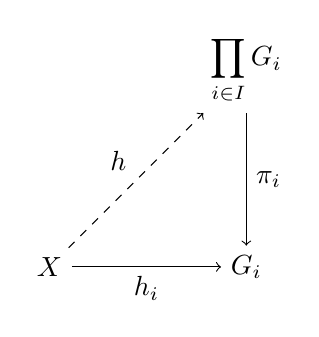
\begin{tikzpicture}[node distance=2.5cm, auto]
	\node (P) {$\displaystyle\prod_{i \in I} \bm{G_i}$};
	\node (Ci) [below of=P] {$\bm{G_i}$};
	\node (X) [left of=Ci] {$\bm{X}$};
	\draw[->] (X) to node [swap] {$h_i$} (Ci);
	\draw[->, dashed] (X) to node {$h$} (P);
	\draw[->] (P) to node {$\pi_i$} (Ci);
\end{tikzpicture}
\end{figure}
\end{prop}
\begin{proof}
Defina a função
	\begin{align*}
	h: X &\to \prod_{i \in I} G_i \\
		x &\mapsto (h_i(x))_{i \in I}.
	\end{align*}
Da propriedade universal para o produto de conjuntos, $h$ é a única função tal que, para todo $i \in I$, $\pi_i \circ h = h_i$. Basta mostrar que $h$ é homomorfismo de grupos. Por simplicidade, apenas a operação $\opb$ em $G$ será explicitada. Sejam $x_1,x_2 \in X$. Então, como $h_i$ são homomorfismos de grupo,
	\begin{equation*}
	h(x_1 \star x_2) = (h_i(x_1 \star x_2))_{i \in I} = (h_i(x_1) \opb_i h_i(x_2))_{i \in I} = h(x_1) \opb h(x_2).
	\end{equation*}
\end{proof}

\subsection{Grupo Livre}

\begin{defi}
Seja $C$ um conjunto. O \emph{conjunto de inversos formais} de $C$ é o conjunto
	\begin{equation*}
	C\inv \coloneqq \set{(c,-1)}{c \in G}.
	\end{equation*}
Os elementos de $C\inv$ são denotados $c\inv \coloneqq (c,-1)$.

Uma \emph{palavra} em $C$ é uma sequência finita $(c_1,\ldots,c_n) \in C^n$. Denota-se $c_1 \cdots c_n$.
\end{defi}

Seja $p=c_1 \cdots c_n$ uma palavra em $C$. A \emph{palavra inversa} de $p$ é a palavra $p\inv \coloneqq c_n\inv \cdots c_1\inv$.

\begin{defi}
Seja $C$ um conjunto e $p_1,p_2 $ palavras em $C \cup C\inv$. A relação de equivalência entre as palavras $p_1$ e $p_2$ é definida por
	\begin{equation*}
	p_1 \sim p_2 \sse p_1p_2\inv \leadsto e.
	\end{equation*}	
\end{defi}

	\begin{equation*}
	C^* \coloneqq \bigcup_{n \in \N} (C \cup C\inv)^n
	\end{equation*}
 Define-se $C^0 = \{e\coloneqq \emptyset\}$.

	\begin{equation*}
	\ger{C} \coloneqq C^*/\sim
	\end{equation*}
	
	A inclusão é definida.
	\func{\iota}{C}{\ger{C}}{c}{[c].}

\begin{prop}[Propriedade Universal]
Seja $C$ um conjunto, $\bm X = (X,\star)$ um grupo e $f: C \to X$ uma função. Então existe um único homomorfismo de grupos $h: \bm{\ger{C}} \to \bm X$ tal que $h \circ \iota = f$ (o diagrama comuta).
\begin{figure}
\centering
\begin{tikzpicture}[node distance=2.5cm, auto]
	\node (C) {$C$};
	\node (G) [above of=C] {$\displaystyle\bm{\ger{C}}$};
	\node (X) [right of=C] {$\bm X$};
	\draw[->] (C) to node [swap] {$f$} (X);
	\draw[->, dashed] (G) to node {$h$} (X);
	\draw[->] (C) to node {$\iota$} (G);
\end{tikzpicture}
\end{figure}
\end{prop}
\begin{proof}
Defina a função \func{h}{\ger{C}}{X}{\left[c_1 \cdots c_n\right] }{f(c_1) \star \cdots \star f(c_n),} de modo que $h([e])=e_X$. Então, para todo $c \in C$,
	\begin{equation*}
	h \circ \iota(c) = h (\iota(c)) = h([c])=f(c).
	\end{equation*}
Logo $h \circ \iota = f$. Para mostrar que é um homomorfismo de grupos, sejam $[c_1 \cdots c_n],$ $[d_1 \cdots d_m] \in \ger{C}$. Então
	\begin{align*}
	h([c_1 \cdots c_n][d_1 \cdots d_m]) &= h([c_1 \cdots c_nd_1 \cdots d_m]) \\
		&= f(c_1) \star \cdots \star f(c_n) \star f(d_1) \star \cdots  \star f(d_m) \\
		&= h([c_1 \cdots c_n]) \star h([d_1 \cdots d_m]).
	\end{align*}
Isso mostra a existência. Para mostrar a unicidade, seja $\overline h: \bm{\ger{C}} \to \bm X$ um homomorfismo de grupos tal que $\overline h \circ \iota = f$. Seja $[c_1 \cdots c_n] \in \ger{C}$. Como $[c_1 \cdots c_n] = [c_1] \cdots [c_n] = \iota(c_1) \cdots \iota(c_n)$, segue que
	\begin{align*}
	\overline h ([c_1 \cdots c_n]) &= \overline h(\iota(c_1) \cdots \iota(c_n)) \\
		&= \overline h(\iota(c_1)) \star \cdots \star \overline h(\iota(c_n)) \\
		&= f(c_1) \star \cdots \star f(c_n) \\
		&= h([c_1 \cdots c_n]),
	\end{align*}
o que implica que $\overline h = h$.
\end{proof}

\subsection{Coproduto de Grupos}

\begin{defi}
Seja $(\bm{G_i})_{i \in I}$ uma família de grupos. O \emph{coproduto} da família $(\bm{G_i})_{i \in I}$ é o par
	\begin{equation*}
	\coprod_{i \in I} \bm{G_i} \coloneqq \left(G,\opb \right),
	\end{equation*}
em que $G \coloneqq \ger{\coprod_{i \in I} G_i}$ é o grupo livre sobre o coproduto de conjuntos $\coprod_{i \in I} G_i$ e \func{\opb}{G \times G}{G}{([p_1],[p_2])}{[p_1p_2].}
\end{defi}

\begin{prop}[Propriedade Universal]
Sejam $(\bm{G_i})_{i \in I}$ uma família de grupos, $\bm X = (X,\star)$ um grupo e, para todo $i \in I$, $h_i: \bm{G_i} \to \bm X$ um homomorfismo de grupos. Então existe um único homomorfismo de grupos $h: \coprod_{i \in I} \bm{G_i} \to \bm X$ tal que, para todo $i \in I$, $h \circ \iota_i = h_i$ (o diagrama comuta).
\begin{figure}
\centering
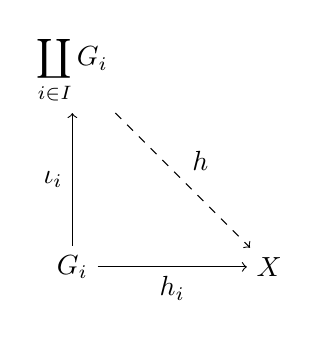
\begin{tikzpicture}[node distance=2.5cm, auto]
	\node (Ci) {$\bm{G_i}$};
	\node (S) [above of=Ci] {$\displaystyle\coprod_{i \in I} \bm{G_i}$};
	\node (X) [right of=Ci] {$\bm X$};
	\draw[->] (Ci) to node [swap] {$h_i$} (X);
	\draw[->, dashed] (S) to node {$h$} (X);
	\draw[->] (Ci) to node {$\iota_i$} (S);
\end{tikzpicture}
\end{figure}
\end{prop}
\begin{proof}
Defina a função \func{h}{\ger{\coprod_{i \in I} G_i}}{X}{\left[(g_1,i_1) \cdots (g_n,i_n)\right]}{h_{i_1}(g_1) \star \cdots \star h_{i_n}(g_n).}

Por simplicidade, seja $G \coloneqq \ger{\coprod_{i \in I} G_i}$. Para mostrar que $h$ é homomorfismo, sejam $[(g_1,i_1) \cdots (g_n,i_n)]$ e $[(g'_1,i'_1) \cdots (g'_m,i'_m)] \in G$. Então
	\begin{align*}
	&h([(g_1,i_1) \cdots (g_n,i_n)][(g'_1,i'_1) \cdots (g'_m,i'_m)]) \\
		&= h([(g_1,i_1) \cdots (g_n,i_n)(g'_1,i'_1) \cdots (g'_m,i'_m)]) \\
		&= h_{i_1}(g_1) \star \cdots \star h_{i_n}(g_n) \star h_{i'_1}(g'_1) \star \cdots \star h_{i'_n}(g'_n) \\
		&= h([(g_1,i_1) \cdots (g_n,i_n)]) \star h([(g'_1,i'_1) \cdots (g'_m,i'_m)]).
	\end{align*}
\end{proof}








































\cleardoublepage
\section{Construções Específicas}

\subsection{Grupo Simples e Subgrupo Normal Maximal}

\begin{defi}
Um \emph{grupo simples} é um grupo não-trivial $\bm G$ cujos únicos subgrupos normais são $\bm{\{e\}}$ e $\bm G$.
\end{defi}

\begin{defi}
Seja $\bm G$ um grupo. Um subgrupo normal \emph{maximal} de $\bm G$ é um subgrupo normal próprio $\bm M \idepro \bm G$ que satisfaz
	\begin{equation*}
	\tag{Maximalidade} \forall \bm N \ide \bm G \qquad M \subseteq N \Rightarrow N = M \ou N = G.
	\end{equation*}
\end{defi}

\begin{prop}
Sejam $\bm G$ um grupo e $\bm M \ide \bm G$ um subgrupo normal. Então $\bm M$ é maximal se, e somente se, $\bm{G/M}$ é simples.
\end{prop}
\begin{proof} Consideremos a projeção canônica
	\begin{align*}
	\pi: G &\to G/M \\
		 g &\mapsto gM.
	\end{align*}
($\Rightarrow$) Suponhamos que $\bm M$ é maximal. Então $\bm M$ é um subgrupo próprio, o implica que $\bm{G/M}$ é não-trivial. Seja $\bm N \ide \bm{G/M}$. Sabemos que $\bm{\pi^{-1}(N)} \ide \bm G$ (\ref{alge:prop.gru.hominv}). Como $[e] \in N$, então $\pi^{-1}(e) \subseteq \pi^{-1}(N)$. Notando que $\pi^{-1}([e])=\nuc(\pi) = M$, segue que $M \subseteq \pi^{-1}(N)$. Como $\bm M$ é maximal, segue que $\pi^{-1}(N) = N$ ou $\pi^{-1}(N) = G$. Notemos que $N=\pi(\pi^{-1}(N))$, pois $\pi$ é sobrejetiva. No primeiro caso, $N = \pi(\pi^{-1}(N)) = \pi(M) = \{[e]\}$. No segundo caso, $N = \pi(\pi^{-1}(N)) = \pi(G) = G/M$. Portanto $\bm{G/M}$ é simples.

\noindent
($\Leftarrow$) Suponhamos que $\bm{G/M}$ é simples. Seja $\bm N \ide \bm G$ tal que $M \subseteq N$. Como $\pi$ é homomorfismo de grupos sobrejetivo, ssegue que $\pi(N) \ide \bm{G/M}$ (\ref{alge:prop.gru.hom}). Como $\bm{G/M}$ é simples, então $\pi(N) = \{[e]\}$ ou $\pi(N) = G/M$. No primeiro caso, $N = \nuc(\pi) = M$. No segundo caso, $N = \pi^{-1}(\pi(N)) = \pi^{-1}(N) = G$. Logo $\bm M$ é maximal.
\end{proof}

\begin{conj}
Sejam $\bm G$ um grupo e $\bm N \idepro \bm G$ um subgrupo normal próprio. Então $\bm G$ tem subgrupo normal maximal.
\end{conj}
\begin{proof}
Usaremos o lema de Zorn. Seja $P \subseteq \p(G)$ o conjunto de todos os subconjuntos $S \subset G$ tais que $\bm S \idepro \bm G$. Então $(P,\subseteq)$ é um conjunto parcialmente ordenado com a contenção de conjuntos usual. Agora, seja $(C)_{i \in I}$ uma cadeia de $(P,\subseteq)$. Consideremos o conjunto $C \coloneqq \bigcup_{i \in I} C_i$. Como 

Notemos que $P$ não é vazio, pois $N \in P$. Seja 



Então $P$ tem elemento maximal.
\end{proof}






\subsection{Sequência subnormal}

\begin{defi}
Seja $\bm G$ um grupo. Uma \emph{sequência subnormal} de $\bm G$ é uma sequência finita $(\bm{N_i})_{i \in \inte_n}$ de subgrupos de $\bm G$ que satisfaz
	\begin{equation*}
	\bm{\{e\}} = \bm{N_0} \ide \cdots \ide \bm{N_n} = \bm G.
	\end{equation*}
O grupo $\bm{N_{i+1}/N_i}$ é o $i$-ésimo \emph{grupo fator} da sequência.
Uma \emph{sequência normal} é uma sequência subnormal em que, para todo $i \in \inte_n$, $\bm{N_i} \ide \bm G$.

Uma sequência subnormal \emph{estrita} de $\bm G$ é uma sequência subnormal $(\bm{N_i})_{i \in \inte_n}$ de $\bm G$ que satisfaz
	\begin{equation*}
	\bm{\{e\}} = \bm{N_0} \idepro \cdots \idepro \bm{N_n} = \bm G.
	\end{equation*}
	
O comprimento
\end{defi}



\subsection{Conjunto gerador}

\begin{defi}
Seja $\bm G$ um grupo e $S \subseteq G$ um conjunto. O grupo \emph{gerado} por $S$ é o grupo $\bm{\langle S \rangle} \leq \bm G$ em que
	\begin{equation*}
	\langle S \rangle \coloneqq \{s_1 \cdots s_n : n \in \N,\ s_i \in S \ou s_i\inv \in S\}.
	\end{equation*}
	\begin{equation*}
	\langle S \rangle \coloneqq \left\{\bigopb_{i \in \inte_n} s_i : n \in \N,\ s_i \in S \ou s_i\inv \in S\right\}.
	\end{equation*}
\noindent
Um \emph{conjunto gerador} de $\bm G$ é um conjunto $S \subseteq G$ tal que $\langle S \rangle = G$.
\end{defi}










\subsection{Grupos Simétricos e Alternados}

\begin{defi}
Seja $C$ um conjunto. O \emph{grupo simétrico} de $C$ é o par $\bm{\simm{C}} = (\simm{C},\circ)$, em que	
	\begin{equation*}
	\simm{C} \coloneqq \set{p: C \to C}{\exists p\inv: C \to C}
	\end{equation*}
é o conjunto de todas as bijeções entre $C$ e $C$, e $\circ$ é a composição de funções. Seja $\alpha$ um número cardinal. Para $C = \alpha$, usa-se a notação $\sime_{\alpha} \coloneqq \simm{\alpha}$.
\end{defi}

\begin{prop}
	Seja $C$ um conjunto. O grupo simétrico $\bm{\simm{C}}$ é um grupo.
\end{prop}
\begin{proof}
	Se $C=\emptyset$, então $\simm{C}=\{\emptyset\}$. Assim, como $\emptyset \circ \emptyset = \emptyset$, segue que $\circ$ é operação binária em $\{\emptyset\}$. Ainda, segue que $\circ$ é associativa, pois $(\emptyset \circ \emptyset) \circ \emptyset = \emptyset \circ (\emptyset \circ \emptyset)$; tem elemeno neutro $\emptyset$, pois $\emptyset \circ \emptyset = \emptyset$, e que todo elemento tem inverso, pois $\emptyset\inv = \emptyset$.

	Suponhamos, então, que $C \neq \emptyset$ e sejam $p_1,p_2 \in \simm{C}$. Como $p_1$ e $p_2$ são bijeções, a função $p_2 \circ p_1: C \to C$ é uma bijeção entre $C$ e $C$ (\ref{prop:comp.func.inj} e \ref{prop:comp.func.sobr}) e, portanto, $p_2 \circ p_1 \in \simm{C}$. Isso mostra que $\circ$ é uma operação binária em $\simm{C}$. A composição de funções é associativa, pois, para todos $p_1,p_2,p_3 \in \simm{C}$, $p_3 \circ (p_2 \circ p_1) = (p_3 \circ p_2) \circ p_1$ (\ref{prop:comp.func.asso}). Ainda, notemos que $\id_C$ é o elemento neutro de $\bm{\simm{C}}$, pois, para todo $p \in \simm{C}$, vale $p \circ \id_C = \id_C \circ p = p$ (\ref{prop:id.comp.func}). Por fim, como $p$ é uma bijeção, existe função inversa $p\inv: C \to C$ que é bijeção entre $C$ e $C$ (\ref{prop:func.inv.esq} e \ref{prop:func.inv.dir}); logo existe $p\inv \in \simm{C}$ tal que $p \circ p\inv = p\inv \circ p = \id_C$. Portanto concluímos que $\bm{\simm{C}}$ é um grupo.
\end{proof}

\begin{prop}
	Sejam $A$ e $B$ conjuntos tais que $\card{A} = \card{B}$. Então
	\begin{equation*}
	\bm{\simm{A}} \simeq \bm{\simm{B}}.
	\end{equation*}
\end{prop}
\begin{proof}
	Seja $\phi: A \to B$ uma bijeção e considere a função
	\begin{align*}
	h : \simm{A} &\to \simm{B} \\
			p &\mapsto \phi \circ p \circ \phi\inv.
	\end{align*}
Primeiro notemos que $h$ é homomorfismo de grupos. Sejam $p_1,p_2 \in \simm{A}$. Então
	\begin{align*}
	h(p_2 \circ p_1)(c) &= \phi \circ (p_2 \circ p_1) \circ \phi^{-1} \\
			&= \phi \circ (p_2 \circ \phi\inv \circ \phi \circ p_1) \circ \phi^{-1} \\
			&= (\phi \circ p_2 \circ \phi\inv) \circ (\phi \circ p_1 \circ \phi\inv) \\
			&= h(p_2) \circ h(p_1).
	\end{align*}
Portanto $h$ é um homomorfismo de grupos entre $\bm{\simm{A}}$ e $\bm{\simm{B}}$.

Agora notemos que $h$ é uma bijeção. A inversa de $h$ é a função
	\begin{align*}
	h\inv : \simm{B} &\to \simm{A} \\
			p &\mapsto \phi\inv \circ p \circ \phi,
	\end{align*}
pois, para todo $p \in \simm{B}$,
	\begin{align*}
	(h \circ h\inv) (p) &= h (h\inv(p)) \\
			&= \phi \circ h\inv(p) \circ \phi\inv \\
			&= \phi \circ (\phi\inv \circ p \circ \phi) \circ \phi\inv \\
			&= p \\
			&= id_{\simm{B}}(p),
	\end{align*}
o que mostra que $h \circ h\inv = id_{\simm{B}}$, e, para todo $p \in \simm{A}$,
	\begin{align*}
	(h\inv \circ h) (p) &= h\inv (h(p)) \\
			&= \phi\inv \circ h(p) \circ \phi \\
			&= \phi\inv \circ (\phi \circ p \circ \phi\inv) \circ \phi \\
			&= p \\
			&= id_{\simm{A}}(p),
	\end{align*}
o que mostra que $h\inv \circ h = id_{\simm{A}}$. Assim, está provado que $h$ é isomorfismo entre $\bm{\simm{A}}$ e $\bm{\simm{B}}$.
\end{proof}

	Essa proposição mostra que podemos estudar somente os grupos simétricos dos números cardinais, pois isso será equivalente a estudar qualquer grupo simétrico. Em particular, para todo conjunto finito, podemos estudar seu grupo simétrico considerando somente o grupo simétrico $\bm\sime_n$, em que $n$ é o número de elementos do conjunto. A partir de agora, as proposições serão considerando esses grupos $\bm\sime_n$.

\begin{prop}
	Seja $n \in \N$. Então $|\sime_n|=n!$.
\end{prop}

\begin{teo}
	Seja $\bm G$ um grupo. Então
	\begin{equation*}
	\bm G \lesssim \bm{\simm{G}}.
	\end{equation*}
\end{teo}
\begin{proof}
	Consideremos a função
	\begin{align*}
	h: G \to \simm{G} & \\
		g \mapsto h(g): & G \to G \\
									&\ x \mapsto g \opb x \\
	\end{align*}
Primeiro, devemos mostrar que $h(g) \in \simm{G}$, para que $h$ esteja bem definida. Para isso, notemos que $h(g)$ está bem definida, já que, para todo $x \in G$, $g \opb x \in G$. Ainda, $h(g)$ é uma bijeção, pois $h(g)\inv = h(g\inv)$, já que, para todo $x \in G$,
	\begin{equation*}
	(h(g) \circ h(g)\inv)(x) = h(g)((h(g)\inv)(x)) = h(g)(g\inv \opb x) = g \opb g\inv \opb x = x =id_G,
	\end{equation*}
o que mostra que $h(g) \circ h(g)\inv = id_G$, e
	\begin{equation*}
	(h(g)\inv \circ h(g))(x) = h(g)\inv((h(g)(x)) = h(g)\inv(g \opb x) = g\inv \opb g \opb x = x =id_G,
	\end{equation*}
o que mostra que $h(g)\inv \circ h(g) = id_G$. Isso mostra que $h(g)$ é uma bijeção e, portanto, $h(g) \in \simm{G}$.

	Agora, notemos que $h$ é um homomorfismo de grupos, pois, para todos $g_1,g_2 \in G$, segue que, para todo $x \in G$,
	\begin{align*}
	h(g_1 \opb g_2)(x) &= (g_1 \opb g_2) \opb x \\
	&= g_1 \opb (g_2 \opb x) \\
	&= h(g_1)(g_2 \opb x) \\
	&= h(g_1)(h(g_2)(x)) \\
	&= (h(g_1) \circ h(g_2))(x),
	\end{align*}
o que mostra que $h(g_1 \opb g_2) = h(g_1) \circ h(g_2)$. Por fim, notemos que $h$ é injetiva, já que, se $g \in G$ é tal que $h(g)=id_G$, então, para todo $x \in G$,
	\begin{equation*}
	g \opb x = h(g)(x) = id_G(x) = x,
	\end{equation*}
o que mostra que $g=e_G$ e, portanto, que $\nuc(h)=\{e_G\}$.
\end{proof}

	Esse teorema é um teorema muito importante, pois ele mostra que, de certa forma, todo grupo é um subconjunto de permutações. Por causa disso que grupos são pensados como os objetos algébricos que modelam a simetria.

\subsubsection{Permutações e Órbitas}

\begin{defi} Seja $n \in \N$. Uma \emph{permutação} de $n$ objetos é um elemento $p \in \sime_n$, denotado por
	\begin{equation*}
	p = \begin{pmatrix}
				1 & 2 & \cdots & n-1 & n \\
				p(1) & p(2) & \cdots &  p(n-1)  & p(n)
			\end{pmatrix}.
	\end{equation*}
\end{defi}

\begin{nota}
	Seja $n \in \N$. A composição de duas permutações $p_1,p_2 \in \sime_n$, quando representadas na notação acima, é denotada
	\begin{equation*}
	p_2 \circ p_1 = \bigl(\begin{smallmatrix}
				1 & 2 & \cdots & n-1 & n \\
				p_2(1) & p_2(2) & \cdots &  p_2(n-1)  & p_2(n)
			\end{smallmatrix}\bigr)
			\bigl(\begin{smallmatrix}
				1 & 2 & \cdots & n-1 & n \\
				p_1(1) & p_1(2) & \cdots &  p_1(n-1)  & p_1(n)
			\end{smallmatrix}\bigr).
	\end{equation*}
\end{nota}

\begin{defi}
	Sejam $n \in \N$ e $p \in \sime_n$. A \emph{matriz de permutação} de $p$ é a matriz $[p] \in \mathbb M_n (\Z)$ cujas entradas são dadas por
	\begin{equation*}
		[p]_{i,j} = \delta_{i,p(j)} = \begin{cases}
												1 & i=p(j) \\
												0 & i \neq p(j).
												\end{cases}
	\end{equation*}
	O \emph{conjunto das matrizes de permutação} de $\sime_n$ é o conjunto
	\begin{equation*}
		[\sime_n] \coloneqq \{[p] : p \in \sime_n\}.
	\end{equation*}
\end{defi}

\begin{prop}
	Seja $n \in \N$. Então o par $\bm{[\sime_n]}=([\sime_n],\cdot)$, em que $\cdot$ é o produto de matrizes, é um grupo, e
	\begin{equation*}
	\bm{\sime_n} \simeq \bm{[\sime_n]}.
	\end{equation*}
\end{prop}
\begin{proof}
	Primeiro, notemos que, para todos $p,q \in \sime_n$,
	\begin{equation*}
	[p][q]_{i,j} = \bigplus_{k=1}^n [p]_{i,k}[q]_{k,j} = \bigplus_{k=1}^n \delta_{i,p(k)}\delta_{k,p(j)}.
	\end{equation*}
	Mas o produto $\delta_{i,p(k)}\delta_{k,p(j)}$ é igual a 1 se, e somente se, $i=p(k)$ e $k=q(j)$. Como $p$ é bijeção, a segunda consição é equivalente a $p(k)=pq(j)$, e isso mostra que as duas consições são equivalentes a $i=p(k)=pq(j)$. Como $p$ é bijeção, para cada $i \in \inte_n$, $k=p\inv(i)$ é o único $k \in \inte_n$ tal que a condição é satisfeita, e segue que
	\begin{equation*}
	[p][q]_{i,j} = \bigplus_{k=1}^n \delta_{i,p(k)}\delta_{k,p(j)} = \bigplus_{k=1}^n \delta_{i,pq(j)} = [pq]_{i,j}.
	\end{equation*}
e, como $pq \in \sime_n$, então $[p][q]=[pq] \in [\sime_n]$. Isso mostra que o produto de matrizes é uma operação binária em $[\sime_n]$. Agora, disso segue que $[p][p\inv]=[pp\inv]=[id]$

MOATRAR QUE O INVERSO DE P ESTA NO GRUPO




Disso, segue que $\bm{[\sime_n]}$ é um grupo, pois é subgrupo de $\mathbb M_n(\Z)$. Por fim, consideremos a função
	\begin{align*}
	h: \sime_n &\to [\sime_n] \\
			p &\mapsto [p].
	\end{align*}
Note que que $h$ é homomorfismo, pois, para todos $p,q \in \sime_n$,
	\begin{equation*}
	h(pq) = [pq]= [p][q] = h(p)h(q).
	\end{equation*}
Ainda, $h$
\end{proof}

\begin{defi}
	Sejam $n \in \N$, $p \in \sime_n$ e $m \in \inte_n$. A \emph{órbita de $m$ sob $p$} é o conjunto
	\begin{equation*}
	\orb_p(m) \coloneqq \{p^k(m) : k \in \Z\}.
	\end{equation*}
O \emph{período} da órbita $\orb_p(m)$ é o número $\card{\orb_p(m)}$. Uma \emph{órbita trivial} é uma órbita de período $1$. Uma órbita de $p$ é a órbita de um elemento $m \in \inte_n$ sob $p$.

	O \emph{conjunto de órbitas} de $p$ é o conjunto
	\begin{equation*}
	\orb_p \coloneqq \{\orb_p(m) : m \in \inte_n\}.
	\end{equation*}
\end{defi}

\begin{prop}
	Sejam $n \in \N$ e $p \in \sime_n$. O conjunto $\orb_p$ é uma partição de $\inte_n$.
\end{prop}
\begin{proof}
	Primeiro, notemos que $m \in \orb_p(m)$ e, portanto, $\emptyset \nsubseteq \orb_p$. Ainda, $\bigcup_{m \in \inte_n} \orb_p(m) = \inte_n$, já que, para todo $m \in inte_n$, $m \in \orb_p(m)$, o que mostra que $\inte_n \subseteq \bigcup_{m \in \inte_n}$ e, para todo $l \in \bigcup_{m \in \inte_n} \orb_p(m)$, existe $m \in \inte_n$ tal que $l \in \orb_p(m)$ e, portanto, existe $k \in \N$ tal que $l=p^k(m) \in \inte_n$, o que mostra que $\bigcup_{m \in \inte_n} \subseteq \inte_n$. Por fim, sejam $o_1,o_2 \in \orb_p$. Então existem $m_1,m_2 \in \inte_n$ tais que $o_1=\orb_p(m_1)$ e $o_2=\orb_p(m_2)$. Se existe $l \in \orb_p(m_1) \cap \orb_p(m_2)$, então existem $k_1,k_2 \in \Z$ tais que $l=p^{k_1}(m_1)=p^{k_2}(m_2)$. Assim, segue que $m_1=p^{k_2-k_1}(m_2)$ e, portanto, $m_1 \in \orb_p(m_2)$. Mas isso implica que $\orb_p(m_1) \subseteq \orb_p(m_2)$; a inclusão contrária é análoga e concluímos que $\orb_p(m_1) = \orb_p(m_2)$. Logo $\orb_p$ é uma partição de $\inte_n$.
\end{proof}

\subsubsection{Permutações, Ciclos e Transposições}

\begin{defi}
	Sejam $n,k \in \N$. Um \emph{ciclo} de $\sime_n$ é um elemento $c \in \sime_n$ para o qual existe $m \in \inte_n$ tal que, para todo $m' \in \inte_n$, $c(m')=m'$ ou existe $d \in \inte_n$ tal que $m'=c^d(m)$. O \emph{comprimento} de um ciclo é a ordem desse ciclo. Um ciclo $c$ cujo comprimento é $k$ é denotado
	\begin{equation*}
	c = \bigl(m \ c(m) \ c^2(m) \ \cdots \  c^{k-2}(m) \ c^{k-1}(m)\bigr).
	\end{equation*}
\end{defi}


\begin{prop}
	Sejam $n \in \N$.
	\begin{enumerate}
	\item Se $c_1,c_2 \in \sime_n$ são ciclos disjuntos, então $c_2 \circ c_1 = c_1 \circ c_2$.
	\end{enumerate}
\end{prop}

\begin{prop}[Fatoração de Permutação]
	Seja $n \in \N$ e $p \in \sime_n$. Então existem únicos ciclos $c_1,\ldots,c_k \in \sime_n$ disjuntos dois a dois tais que $p=c_1 \circ \cdots \circ c_k$.
\end{prop}
\begin{proof}
	Seja $k \coloneqq \card{\orb_p}$. O cojunto $\orb_p$ particiona $\inte_n$. Sejam $(o_k)_{i \in \inte_k}$ uma indexação de $\orb_p$ e $m_1,\cdot,m_k \in \inte_n$ tais que $o_i=\orb_p(m_i)$ para todo $i \in \inte_k$, e seja $k_i \coloneqq \card{\orb_p(m_i)}$. Definamos $c_i \coloneqq  \bigl( m_i \ \cdots \  p^{k_i-1}(m_i)\bigr)$. Então segue que
	\begin{equation*}
	p = \bigtimes_{i=1}^k \bigl( m_i \ \cdots \  p^{k_i-1}(m_i)\bigr) = \bigtimes_{i=1}^k c_i.
	\end{equation*}
\end{proof}



\subsection{Grupos Cíclicos}

\subsection{Grupos Diedrais}



























\newpage

\chapter{Anéis}

\section{Anel}

\begin{defi}
	Um \emph{anel} é uma tripla $\bm A=(A,+,\cdot)$ em que
	\begin{enumerate}
	\item $(A,+)$ é um grupo comutativo com elemento neutro chamado de \emph{zero} ou \emph{nulidade} e representado por $0$ (ou $0_A$, caso exista ambiguidade).
	\item $(A,\cdot)$ é um monoide comutativo com elemento neutro chamado de \emph{um} ou \emph{unidade} e representado por $1$ (ou $1_A$, caso exista ambiguidade).
	\item A operação $\cdot$ é distributiva sobre $+$.
	\end{enumerate}
As operações $+$ e $\cdot$ são chamadas, respectivamente, de \emph{adição} e \emph{multiplicação}. A imagem de dois elementos $a_1,a_2 \in A$ pela adição é chamada de \emph{soma} de $a_1$ e $a_2$ e denotada por $a_1+a_2$. A imagem de $a_1,a_2$ pela multiplicação é chamada de \emph{produto} de $a_1$ e $a_2$ e denotada por $a_1 \cdot a_1$ ou $a_1a_2$.
\end{defi}

	Um comentário sobre os elementos neutros $0$ e $1$. Se $0=1$, o anel será trivial, mas garantimos esse anel na definição pois, mais para frente, quando virmos anéis quocientes, vai ser proveitoso que qualquer anel quociente seja um anel, e se quocientarmos um anel por ele mesmo, temos o anel trivial.

\begin{nota}
	Como $(A,+)$ é um grupo, denotaremos o inverso de um elemento $a \in A$ sob $+$ por $-a$, e escreveremos $a_1 - a_2$ para $a_1 + (-a_2)$. Ainda, a multiplicação tem preferência na notação; ou seja, $a_1a_2+a_3 = (a_1 \cdot a_2)+a_3$ e $-a_1a_2 = -(a_1 \cdot a_2)$. Denotaremos o inverso de um elemento $a \in A$ sob $\cdot$ por $a^{-1}$, se ele existir, pois sabemos que é único (\ref{prop:unic.inv}). Os símbolos operatórios relativos à adição e à multiplicação serão, respectivamente, $\bigplus$ e $\bigtimes$. Caso não haja ambiguidade, denotaremos um anel pelo símbolo que denota seu conjunto escrito em negrito, como em $\bm A=(A,+,\cdot)$.
\end{nota}

\begin{prop}
	Seja $\bm A$ um anel. Então, para todo $a,b \in A$,
	\begin{enumerate}
	\item $0 \cdot a = 0$;
	\item $-(a \cdot b) = (-a) \cdot b$.
	\end{enumerate}
\end{prop}
\begin{proof}
	\begin{enumerate}
	\item
		\begin{align*}
		0 \cdot a &= 0 \cdot a + 0 \\
			&= 0 \cdot a + (0 \cdot a - 0 \cdot a) \\
			&= (0 \cdot a + 0 \cdot a) - 0 \cdot a \\
			&= (0+0) \cdot a - 0 \cdot a \\
			&= 0 \cdot a - 0 \cdot a \\
			&= 0.
		\end{align*}
	\item
		\begin{align*}
		-(a \cdot b) &= -(a \cdot b) + 0 \\
			&= -(a \cdot b) + 0 \cdot b \\
			&= -(a \cdot b) + (a - a) \cdot b \\
			&= -(a \cdot b) + (a \cdot b + (-a) \cdot b) \\
			&= (-(a \cdot b) + a \cdot b) + (-a) \cdot b \\
			&= 0 + (-a) \cdot b \\
			&= (-a) \cdot b.
		\end{align*}
	\end{enumerate}
\end{proof}

\begin{defi}
	Seja $\bm A$ um anel. O conjunto dos elementos invertíveis sob multiplicação de $\bm A$ é denotado por $A^*$.
\end{defi}

\begin{prop}
	Seja $\bm A$ um anel. O par $(A^*,\cdot|_{A^* \times A^*})$ é um grupo comutativo.
\end{prop}
\begin{proof}
	O par $(A,\cdot)$ é um monoide comutativo com elemento neutro $1$. Portanto segue que o par $(A^*,\cdot|_{A^* \times A^*})$ é um grupo. Como $(A,\cdot)$ é comutativo, então $(A^*,\cdot|_{A^* \times A^*})$ também o é.
\end{proof}

\begin{defi}
	Um \emph{domínio de integridade} (ou \emph{domínio}) é um anel $\bm A$ em que
	\begin{equation*}
	\forall a_1, a_2 \in A \qquad a_1 \cdot a_2 = 0 \Rightarrow a_1=0 \text{\ \ ou\ \ } a_2=0.
	\end{equation*}
\end{defi}

\begin{defi}
	Um \emph{corpo} é um anel $\bm A$ em que $(A \setminus \{0\},\cdot)$ é um grupo.
\end{defi}

\begin{prop}
\label{prop:corp.dom}
	Seja $\bm A$ um corpo. Então $\bm A$ é um domínio.
\end{prop}
\begin{proof}
	Sejam $a_1,a_2 \in A$ tais que $a_1 \cdot a_2=0$. Suponhamos que $a_2 \neq 0$. Então existe $a_2^{-1} \in A$ e temos
	\begin{equation*}
	\begin{split}
	a_1 &= a_1 \cdot 1 \\
		&= a_1 \cdot (a_2 \cdot a_2^{-1}) \\
		&= (a_1 \cdot a_2) \cdot a_2^{-1}\\
		&= 0 \cdot a_2^{-1} \\
		&= 0.
	\end{split}
	\end{equation*}
	Logo, se $a_1 \cdot a_2=0$, $a_1=0$ ou $a_2=0$.
\end{proof}

\begin{prop}[Lei do corte em domínios]
	Seja $\bm A$ um domínio e $a,a_1,a_2 \in A$, $a \neq 0$. Então
	\begin{equation*}
	aa_1 = aa_2 \Rightarrow a_1=a_2
	\end{equation*}
\end{prop}
\begin{proof}
	Se $aa_1 = aa_2$, então $-aa_1 = -aa_2$. Portanto
	\begin{equation*}
	a(a_1-a_2) = aa_1 -aa_2 = aa_1 -aa_1 = 0.
	\end{equation*}
Logo, como $\textbf{A}$ é um domínio e $a \neq 0$, temos que $a_1-a_2=0$, o que implica $a_1=a_2$.
\end{proof}

	Essa proposição é interessante pois, mesmo sem exigir que $(A \setminus \{0\},\cdot)$ seja um grupo, como no caso de $\textbf{A}$ ser um corpo, se $\textbf{A}$ for um domínio, vale a lei do corte da multiplicação para elementos de $A \setminus \{0\}$.

\section{Subanel}

\begin{defi}
Seja $\bm A=(A,+,\times)$ um anel. Um \emph{subanel} de $\bm A$ é um anel $\bm S=(S,+_S,\times_S)$ em que $S \subseteq A$, $+_S = +|_{S \times S}$ e $\times_S = \times|_{S \times S}$. Denota-se $\bm S \leq \bm A$. Um subanel \emph{próprio} de $\bm A$ é um subanel $\bm S \leq \bm A$ em que $S$ é um conjunto próprio de $A$ ($S \subset A$). Denota-se $\bm S < \bm A$.
\end{defi}

\begin{prop}
Sejam $\bm A=(A,+,\times)$ um anel e $S \subseteq A$. Então $\bm S=(S,+|_{S \times S},\times|_{S \times S})$ é um anel com $1 \in S$ se, e somente se,
	\begin{enumerate}
	\item $(S,+|_{S \times S})$ é um subgrupo comutativo de $(A,+)$:
			\begin{enumerate}
			\item (Não-vacuidade) $S \neq \emptyset$;
			\item (Fechamento) $\forall s_1,s_2 \in S \qquad s_1 + s_2 \in S$;
			\item (Invertibilidade) $\forall s \in S \qquad -s \in S$;
			\end{enumerate}
	\item $(S,\times|_{S \times S})$ é um submonoide comutativo de $(A,\times)$ com $1 \in S$:
			\begin{enumerate}
			\item (Identidade) $1 \in S$;
			\item (Fechamento) $\forall s_1,s_2 \in S \qquad s_1 \times s_2 \in S$.
			\end{enumerate}
	\end{enumerate}
\end{prop}
\begin{proof}
($\Rightarrow$) Suponhamos que $\bm S$ é um anel com $1 \in S$.
(Subgrupo) Como $S \subseteq A$ e $(S,+|_{S \times S})$ um grupo comutativo, então é um subgrupo de $(A,+)$ por definição de subgrupo (o que é equivalente às propriedades listadas) e é comutativo (\ref{alge:prop.subgru})).
(Subanel)  Como $S \subseteq A$ e $(S,\times|_{S \times S})$ um monoide comutativo com $1 \in S$, então é um submonoide de $(A,\times)$ por definição de submonoide (o que é equivalente às propriedades listadas) e é comutativo (\ref{alge:prop.submon}).

($\Leftarrow$) Suponhamos, agora, que $(S,+|_{S \times S})$ é subgrupo comutativo de $(A,+)$ e $(S,\times_{S \times S})$ é submonoide comutativo de $(A,\times)$.
(Grupo comutativo) Como $(S,+|_{S \times S})$ é subgrupo comutativo, então é um grupo comutativo por definição de subgrupo. (Monoide comutativo) Como $(S,\times|_{S \times S})$ é submonoide comutativo, então é um monoide comutativo por definição de monoide. (Distributividade) Sejam $s_1,s_2,s_3 \in S$. Então
	\begin{align*}
	s_1 \times|_{S \times S} (s_2 +|_{S \times S} s_3) &= s_1 \times (s_2 + s_3) \\
		&= (s_1 \times s_2) + (s_1 \times s_3) \\
		&= (s_1 \times| _{S \times S} s_2) +|_{S \times S} (s_1 \times|_{S \times S} s_3).
	\end{align*}
Logo $\times_{S \times S}$ é distributiva sobre $+ \times_{S \times S}$.

\end{proof}

\section{Anel de Polinômios}

\begin{defi}
	Seja $\bm A$ um anel. O \emph{conjunto dos polinômios em $A$} é o conjunto
	\begin{equation*}
	A[x] \coloneqq \set{\bigplus_{i=0}^m a_ix^i}{a_i \in A, m \geq 0},
	\end{equation*}
em que $a_0x^0 \coloneqq a_0$. Os números $a_i$ são chamados de coeficientes do polinômio. Dizemos que dois polinômios são iguais se todos seus coeficientes não nulos são iguais.
\end{defi}

\begin{defi}
	 Seja $\bm A$ um anel e $f,g \in A[x]$ tais que $f \coloneqq \bigplus_{i=0}^m a_ix^i$ e $g \coloneqq \bigplus_{i=0}^n b_ix^i$. Então definimos as operações binárias $\oplus$ e $\odot$ em $A[x]$ por
	\begin{equation*}
	f \oplus g \coloneqq \bigplus_{i=0}^{\max\{m,n\}} (a_i+b_i)x^i
	\qquad \qquad f \odot g \coloneqq \bigplus_{i=0}^{m+n} \left(\bigplus_{j=0}^i a_jb_{i-j}\right)x^i.
	\end{equation*}
tal que $a_i=0$ para $m < i \leq \max\{m,n\}$ e $b_i=0$ para $n < i \leq \max\{m,n\}$. Denotaremos $\oplus$ e $\odot$ por $+$ e $\cdot$ quando não existir ambiguidade.
\end{defi}

\begin{prop}
	Seja $\bm A=(A,+,\cdot)$ um anel. Então $\bm{A[x]} \coloneqq (A[x],\oplus,\odot)$ é um anel.
\end{prop}
\begin{proof}
	Sejam $f,g,h \in A[x]$ tais que $f \coloneqq \bigplus_{i=0}^m a_ix^i$, $g \coloneqq \bigplus_{i=0}^n b_ix^i$ e $h \coloneqq \bigplus_{i=0}^l c_ix^i$. Notemos que $\max\{\max\{m,n\},l\}=\max\{m,\max\{n,l\}\}$. Denotamos essa quantidade como $\max\{m,n,l\}$. Definamos $a_i=0$ para $m < i \leq \max\{m,n,l\}$, $b_i=0$ para $n < i \leq \max\{m,n,l\}$ e $c_i=0$ para $l < i \leq \max\{m,n,l\}$.

	Primeiro vamos mostrar que $(A[x],\oplus)$ é um grupo comutativo. Todas as propriedades de grupo comutativo decorrem do fato de que $(A,+)$ é um grupo comutativo com elemento neutro $0$. A operação $\oplus$ é associativa, pois
	\begin{equation*}
	\begin{split}
	(f \oplus g) \oplus h &= \left( \bigplus_{i=0}^{\max\{m,n\}} (a_i+b_i)x^i \right) \oplus h \\
		&= \left( \bigplus_{i=0}^{\max\{m,n,l\}} ((a_i+b_i)+c_i)x^i \right) \\
		&= \left( \bigplus_{i=0}^{\max\{m,n,l\}} (a_i+(b_i+c_i))x^i \right) \\
		&= f \oplus \left( \bigplus_{i=0}^{\max\{n,l\}} (b_i+c_i)x^i \right) \\
		&= f \oplus (g \oplus h),
	 \end{split}
	 \end{equation*}
e comutativa, pois
	 \begin{equation*}
	f \oplus g = \bigplus_{i=0}^{\max\{m,n\}} (a_i+b_i)x^i = \bigplus_{i=0}^{\max\{m,n\}} (b_i+a_i)x^i = g \oplus f.
	 \end{equation*}
Ainda, o polinômio $0_{A[x]} \coloneqq 0$ é elemento neutro, pois
	\begin{equation*}
	f \oplus 0_{A[x]} = \bigplus_{i=0}^{\max\{m,0\}} (a_i+0)x^i = \bigplus_{i=0}^m a_ix^i = f.
	 \end{equation*}
Por fim, existe $-a_i \in A$ para todo $i \in \{0, \ldots, m\}$. Assim, $-f \coloneq \bigplus_{i=0}^m (-a_i)x^i$ é o polinômio inverso de $f$, pois
	\begin{equation*}
	f+(-f) = \bigplus_{i=0}^{\max\{m,m\}} (a_i+(-a_i))x^i = \bigplus_{i=0}^m 0x^i = 0
	\end{equation*}

	Agora, devemos mostrar que $(A[x],\odot)$ é um monoide comutativo. Novamente, as propriedades decorrem do fato de que $(A,\cdot)$ é um monoide comutativo com elemento neutro $1$. A operação $\odot$ é associativa, pois
	\begin{equation*}
	\begin{split}
	(f \odot g) \odot h &= \left( \bigplus_{i=0}^{m+n} \left(\bigplus_{j=0}^i a_jb_{i-j}\right)x^i \right) \odot h \\
		&= \bigplus_{i=0}^{m+n+l} \left( \bigplus_{j=0}^{i}\left(\bigplus_{k=0}^j a_kb_{j-k}\right)c_{i-j}\right)x^i \\
		&= \bigplus_{i=0}^{m+n+l} \left( \bigplus_{j=0}^{i}\left(\bigplus_{k=0}^j a_kb_{j-k}\right)c_{i-j}\right)x^i \\
		&= \\
		&= \bigplus_{i=0}^{m+n+l} \left( \right) \\
		&= f \odot \left( \bigplus_{i=0}^{n+l} \left(\bigplus_{j=0}^i b_jc_{i-j}\right)x^i \right) \\
		&= f \odot (g \odot h).
	 \end{split}
	 \end{equation*}
e comutativa, pois
	\begin{equation*}
	f \odot g = \bigplus_{i=0}^{m+n} \left(\bigplus_{j=0}^i a_jb_{i-j}\right)x^i = \bigplus_{i=0}^{n+m} \left(\bigplus_{j=0}^i b_ja_{i-j}\right)x^i = g \odot f.
	 \end{equation*}
Ainda, o polinômio $1_{A[x]} \coloneqq 1$ é elemento neutro, pois
	\begin{equation*}
	f \odot 1_{A[x]} = \bigplus_{i=0}^{m+0} \left(\left(\bigplus_{j=0}^{i-1} a_j \cdot 0 \right) + a_i \cdot 1\right)x^i = \bigplus_{i=0}^m a_ix^i = f.
	 \end{equation*}

	 Por fim, distributividade...
\end{proof}

\begin{defi}
	Definimos o \emph{grau} de um polinômio $f \in A[x] \subseteq \{0\}$ como o maior índice de um coeficiente não nulo de $f$; ou seja, se $f=\bigplus_{i=0}^m a_ix^i$ com $a_m \neq 0$, então $\g(f)=m$.
\end{defi}

\begin{prop}
	Seja $\bm A=(A,+,\cdot)$ um domínio e $f,g \in A[x]\setminus\{0\}$. Então
	\begin{equation*}
	\g(fg)=\g(f)+\g(g).
	\end{equation*}
\end{prop}
\begin{proof}
	Sejam $\g(f)=m$ e $\g(g)=n$, e sejam $f = \bigplus_{i=0}^m a_ix^i$ e $g = \bigplus_{i=0}^n b_ix^i$. O produto $fg$ terá coeficientes $\bigplus_{j=0}^i a_jb_{i-j}$, com $i \in \{0,\ldots,m+n\}$. Notemos que, para $i = m+n$, $\bigplus_{j=0}^i a_jb_{i-j} = a_mb_n$. Isso ocorre porque todos os termos desse somatório se anulam, menos quando $j=m$. Se $j>m$, temos $a_j=0$; se $j<m$, então $i-j > m+n-m = n$, e temos $b_{i-j}=0$. Em ambos os casos, $a_jb_{i-j}=0$. Portanto $\bigplus_{j=0}^{m+n} a_jb_{i-j}c= a_mb_n$. Como $m$ e $n$ são os graus de $f$ e $g$, respectivamente, sabemos que $a_m \neq 0$ e $b_n \neq 0$ e, como $\bm A$ é um domínio, isso implica que $a_mb_n \neq 0$ Logo $fg \neq 0$ e $\g(fg)=m+n$.
\end{proof}

\begin{prop}
	Seja $\bm A=(A,+,\cdot)$ um anel. Então $\bm A$ é um domínio se, e somente se, $\bm{A[x]}=(A[x],+,\cdot)$ é um domínio.
\end{prop}
\begin{proof}
	Suponha que $\bm A$ é um domínio e sejam $f,g \in A[x]\setminus\{0\}$. Então $\g(fg)=\g(f)+\g(g)$, o que mostra que $fg \neq 0$. Logo $\bm{A[x]}$ é um domínio. Por outro lado, suponha que $\bm{A[x]}$ é um domínio e sejam $a_1,a_2 \in A\setminus\{0\}$. Então $a_1,a_2 \in A[x]\setminus\{0\}$ e, portanto, $a_1a_2 \neq 0$. Logo $\bm A$ é um domínio.
\end{proof}

Podemos ver que $\bm{A[x]}$ nunca é um corpo, pois $x$ não tem inverso.

\section{Produto de Anéis}

\begin{defi}
Seja $(\bm{A_i})_{i \in I}=(A_i,+_i,\times_i)_{i \in I}$ uma família de anéis. O \emph{produto} da família $(\bm{A_i})_{i \in I}$ é a tripla
	\begin{equation*}
	\prod_{i \in I} \bm{A_i} \coloneqq (A,+,\times)
	\end{equation*}
em que $A = \prod_{i \in I} A_i$ é o produto de conjuntos, \func{+}{A \times A}{A}{(a,b)}{(a_i +_i b_i)_{i \in I}} e \func{\times}{A \times A}{A}{(a,b)}{(a_i \times_i b_i)_{i \in I}.}
Denotaremos as operações $+_i$ todas por $+$ e as operações $\times_i$ todas por $\times$ quando não existir ambiguidade.
\end{defi}

\begin{prop}
Seja $(\bm{A_i})_{i \in I}=(A_i,+_i,\times_i)_{i \in I}$ uma família de anéis. Então o produto $\prod_{i \in I}\bm{A_i}$ é um anel.
\end{prop}
\begin{proof}
Como,  para todo $i \in I$, o par $(A_i,+_i)$ é um grupo comutativo, segue que o par $\left(\prod_{i \in I} A_i,+ \right)$ é um grupo comutativo.

Agora, devemos mostrar que $\left( \prod_{i=1}^n A_i,\times \right)$ é um monoide comutativo. Novamente, as popriedades de monoide comutativo decorrem do fato de que $(A_i,\times_i)$, $i \in I$, são todos monoides comutativos com elementos neutros $1_i$, respectivamente. Sejam $a=(a_i)_{i \in I}, b=(b_i)_{i \in I}, c=(c_i)_{i \in I} \in \prod_{i \in I} A_i$. A operação $\times$ é associativa, pois
	\begin{align*}
	(a \times b) \times c &= (a_i \times_i b_i)_{i \in I} \times c \\
		&= ((a_i \times_i b_i) \times_i c_i)_{i \in I} \\
		&= (a_i \times_i (b_i \times_i c_i))_{i \in I} \\
		&= a \times (b_i \times_i c_i)_{i \in I} \\
		&= a \times (b \times c),
	\end{align*}
e comutativa, pois
	\begin{equation*}
	a \times b = (a_i \times_i b_i)_{i \in I} = (b_i \times_i a_i)_{i \in I} = b \times a.
	\end{equation*}
Ainda, $1 \coloneqq (1_i)_{i \in I}$ é elemento neutro, pois
	\begin{equation*}
	a \times 1 = (a_i \times 1_i)_{i \in I} = (a_i)_{i \in I} = a.
	\end{equation*}

	Por fim, como $\times_i$ são ditributivas sobre $+_i$, temos que
	\begin{align*}
	a \times (b + c) &= a \times (b_i +_i c_i)_{i \in I} \\
		&= (a_i \times_i (b_i +_i c_i))_{i \in I} \\
		&= ((a_i \times_i b_i) +_i (a_i \times_i c_i))_{i \in I} \\
		&= (a_i \times_i b_i)_{i \in I} + (a_i \times_i c_i)_{i \in I} \\
		&= (a \times b) + (a \times c).
	\end{align*}
\end{proof}

\section{Ideais e Anéis Quocientes}

\begin{defi}
	Seja $\bm A$ um anel. Um \emph{ideal} de $\bm A$ é um conjunto não vazio $I \subseteq A$ tal que
	\begin{enumerate}
	\item $\forall i_1,i_2 \in I \qquad i_1 - i_2 \in I$
	\item $\forall a \in A, i \in I \qquad ai \in I$
	\end{enumerate}
Denotamos que $I$ é ideal de $\bm A$ por $I \ide A$. Ainda, $I \idepro A$ significa que $I \neq A$ e $I \ide A$.
\end{defi}

	É interessante observar que $I$ é subgrupo de $(A,+)$. A definição de ideal difere da definição de subanel na propriedade 2.

\begin{prop}
	Sejam $\bm A$ um anel e $I \ide A$. Então
	\begin{enumerate}
	\item $0 \in I$;
	\item $\forall i_1,i_2 \in I \qquad i_1 + i_2 \in I$;
	\item $1 \in I \Rightarrow I=A$;
	\item $\{0\}$ e $A$ são ideais de $A$.
	\end{enumerate}
\end{prop}
\begin{proof}
	\begin{enumerate}
	\item Seja $i \in I$. Então $0 = i-i \in I$.
	\item Sejam $i_1,i_2 \in I$. Pelo item anterior, sabemos que $0 \in I$, o que implica $-i_2 = 0 - i_2 \in I$. Logo $i_1 + i_2 = i_1 - (-i_2) \in I$.
	\item Se $1 \in I \ide A$, então, para todo $a \in A$, temos $a=a\cdot1 \in A$. Logo $I=A$.
	\item Consideremos $\{0\}$. Se $i \in \{0\}$, então $i=0$. Portanto, para todo $a \in A$ e $i \in \{0\}$, temos $i-i=0 \in \{0\}$ e $ai=0 \in \{0\}$. Logo $\{0\} \ide A$. Agora, consideremos $A$. Para todo $a_1,a_2 \in A$, temos $a_1-a_2 \in A$ e $a_1a_2 \in A$. Logo $A \ide A$.
	\end{enumerate}
\end{proof}

\begin{prop}
	Sejam $\bm A$ um anel e $(I_j)_{j \in J}$ uma família de ideais de $\bm A$. Então
	\begin{equation*}
	I \coloneqq \bigcap_{j \in J} I_j
	\end{equation*}
é um ideal de $\bm A$.
\end{prop}
\begin{proof}
	Sejam $i_1,i_2 \in I$ e $a \in A$. Então, para todo $j \in J$, $i_1,i_2 \in I_j$ e, como $I_j$ é ideal de $\bm A$, segue que $i_1-i_2 \in I_j$ e que $ai_1 \in W_i$. Logo $i_1-i_2 \in I$ e $ai_1 \in I$, o que mostra que $I$ é ideal de $\bm A$.
\end{proof}

\begin{prop}
	Sejam $\bm A$ um anel e $(I_j)_{n \in \N}$ uma sequência crescente de ideais de $\bm A$; ou seja, $I_1 \subseteq I_2 \subseteq \cdots \subseteq I_n \subseteq \cdots$. Então
	\begin{equation*}
	I \coloneqq \bigcup_{n \in \N} W_n
	\end{equation*}
é um ideal de $\bm A$.
\end{prop}
\begin{proof}
	Sejam $i_1,i_2 \in I$. Então existem $n,m \in \N$ tais que $i_1 \in I_n$ e $i_2 \in I_m$. Nesse caso, $I_n \subseteq I_m$ ou $I_m \subseteq I_n$. Sem perda de generalidade, suponhamos o primeiro caso. Então segue que $i_1 \in I_m$ e, portanto, $i_1-i_2 \in I_m$, o que mostra que $i_1-i_2 \in I$. Agora, seja $a \in A$ e notemos que, como $I_n$ é ideal de $\bm A$, segue qque $ai_1 \in I_n$. Logo $ai_1 \in I$, o que mostra que $I$ é ideal de $\bm A$.
\end{proof}


\begin{defi}
	Sejam $\bm A$ um anel e $a_1,\ldots,a_n \in A$. Definimos o conjunto
	\begin{equation*}
	\bigplus_{i=1}^n a_iA = a_1A + \ldots + a_nA \coloneqq \set{\bigplus_{i=1}^n a_ib_i}{b_i \in A}.
	\end{equation*}
\end{defi}

\begin{prop}
	Sejam $\bm A$ um anel e $a_1,\ldots,a_n \in A$. Então
	\begin{equation*}
	I \coloneqq \bigplus_{k=1}^n a_kA \ide A.
	\end{equation*}
\end{prop}
\begin{proof}
	Sejam $a \in A$ e $i_1,i_2 \in I$ tais que $i_1=\bigplus_{k=1}^n a_ib_i$ e $i_2=\bigplus_{k=1}^n a_ic_i$. Então
	\begin{equation*}
	i_1-i_2=\bigplus_{k=1}^n a_kb_k - \bigplus_{k=1}^n a_kc_k = \bigplus_{k=1}^n a_k(b_k-c_k) \in I,
	\end{equation*}
pois $(b_k-c_k) \in A$ para todo $k \in \{1,\ldots,n\}$. Ainda,
	\begin{equation*}
	ak_1=a\bigplus_{k=1}^n a_kb_k= \bigplus_{k=1}^n a_k(ab_k) \in I,
	\end{equation*}
pois $ab_k \in A$ para todo $k \in \{1,\ldots,n\}$. Logo $I \ide A$.
\end{proof}

	Esse ideal é chamado de ideal de $A$ gerado por $a_1,\ldots,a_n$.

\begin{defi}
	Seja $\bm A$ um anel. Um \emph{ideal principal} de $\bm A$ é um ideal $I \ide A$ tal que
	\begin{enumerate}
	\item $\exists a \in A \qquad I=aA$.
	\end{enumerate}
\end{defi}

\begin{prop}
\label{pro:corp.sse.ide}
	Seja $\bm A$ um anel. Então $\bm A$ é um corpo se, e somente se, $\bm A$ é um anel não-trivial cujos únicos ideais de $\bm A$ são $\{0\}$ e $A$.
\end{prop}
\begin{proof}
	Suponha que $\bm A$ é um corpo. Então $(A\setminus\{0\},\cdot)$ é um grupo e, portanto, $A \neq \emptyset$. Seja $I \ide A$ e suponha que $I \neq \{0\}$. Então existe $i \in I\setminus\{0\}$. Como $\bm A$ é corpo, existe $i^{-1} \in A$. Portanto $1=i^{-1}i \in I$. Logo $I=A$.

	Por outro lado, suponha que os únicos ideais de $A$ são $\{0\}$ e $A$. Como $\bm A$ é não-trivial, seja $a \in A\setminus\{0\}$ e consideremos o ideal $I=aA$. Notemos que $a=a \cdot 1 \in aA$, o que implica $I \neq \{0\}$. Portanto $I=A$. Mas então $1 \in aA$, o que significa que deve existir $b \in A$ tal que $1=ab$; ou seja, todo $a \in A\setminus\{0\}$ tem inverso em $A$. Logo $\bm A$ é corpo.
\end{proof}

\begin{prop}
	Sejam $\bm A$ um anel e $I \ide A$. A relação binária $\sim_I$ em $A$, definida por
	\begin{equation*}
	a \sim_I b \Leftrightarrow a-b \in I,
	\end{equation*}
é uma relação de equivalência.
\end{prop}
\begin{proof} Vamos demonstrar as três propriedades de uma relação de equivalência.
	\begin{enumerate}
	\item (Reflexividade) Seja $a \in A$. Então $a-a=0 \in I$. Logo $a \sim_I a$.
	\item (Simetria) Sejam $a_1,a_2 \in A$ tais que $a_1 \sim_I a_2$. Então $(a_1-a_2) \in I$. Mas $0 \in I$, o que implica $a_2-a_1 = 0-(a_1-a_2) \in I$. Logo $a_2 \sim_I a_1$.
	\item (Transitividade) Sejam $a_1,a_2,a_3 \in A$ tais que $a_1 \sim_I a_2$ e $a_2 \sim_I a_3$. Então $(a_1-a_2),(a_2-a_3) \in I$, o que implica $a_1-a_3=(a_1-a_2)+(a_2-a_3) \in I$. Logo $a_1 \sim_I a_3$.
	\end{enumerate}
\end{proof}

\begin{defi}
	Sejam $\bm A$ um anel e $I \ide A$. O conjunto $a+I \coloneqq \{a+i : i \in I\}$ é a \emph{classe lateral} de $I$ com representante $a$. O conjunto das classes laterais de $A$ é denotado por $A/I \coloneqq \{a+I : a \in A\}$.
\end{defi}

\begin{prop}
	Sejam $(A,+,\cdot)$ um anel, $I \ide A$ e $\sim_I$ a relação de equivalência definida na proposição anterior e $a \in A$. Então a classe de equivalência $[a]=\{b \in A : b \sim_I a\}$ é igual à classe lateral $a+I$ e, por consequência, o conjunto quociente $A/\sim_I$ é igual ao conjunto $A/I$.
\end{prop}
\begin{proof}
	Seja $b \in [a]$. Então $b-a \in I$; ou seja, existe $i \in I$ tal que $b-a=i$. Mas isso implica $b=a+i$, que implica, por sua vez, que $b \in a+I$. Por outro lado, seja $b \in a+I$. Então existe $i \in I$ tal que $b=a+i$; ou seja, $b-a=i$, que implica $b-a \in I$ e, assim, $b \in [a]$. Disso, vem que $A/\sim_I = A/I$.
\end{proof}

	Uma consequência disso é que o conjunto $A$ é particionado em classes laterais de $I$. Outra consequência é que duas classes laterais são iguais se, e somente se, a diferença entre seus representantes está em $I$.

\begin{defi}
	Sejam $\bm A$ um anel, $I \ide A$ e $a_1,a_2 \in A$. Então definimos as operações binárias $\oplus$ e $\odot$ em $A/I$ por
	\begin{equation*}
	(a_1+I) \oplus (a_2+I) \coloneqq (a_1+a_2)+I \qquad \qquad (a_1+I) \odot (a_2+I) \coloneqq (a_1 \cdot a_2)+I
	\end{equation*}
Denotaremos $\oplus$ e $\odot$ por $+$ e $\cdot$ quando não existir ambiguidade.
\end{defi}

\begin{prop}
	As operações $\oplus$ e $\odot$ da definição anterior estão bem definidas.
\end{prop}
\begin{proof}
	Sejam $a_1,a_2,b_1,b_2 \in A$ tais que $a_1+I=a_2+I$ e $b_1+I=b_2+I$. Primeiro, vamos mostrar que $\oplus$ está bem definida. Devemos mostrar que $(a_1+b_1)+I=(a_2+b_2)+I$. De $a_1+I=a_2+I$, sabemos que $a_1-a_2 \in I$. Da mesma forma, $b_1-b_2 \in I$. Mas então $(a_1+b_1)-(a_2+b_2) = (a_1-a_2)+(b_1-b_2) \in I$, o que implica $(a_1+b_1)+I=(a_2+b_2)+I$.

	Agora, vamos mostrar que $\odot$ está bem definida. Devemos mostrar que $(a_1b_1)+I=(a_2b_2)+I$. Sejam $c=a_1-a_2$ e $d=b_1-b_2$. Notemos que
	\begin{equation*}
	a_1b_1 = (a_2+c)(b_2+d) = a_2b_2 + a_2d + cb_2 + cd.
	\end{equation*}
Como $c,d \in I$, $(a_2d + cb_2 + cd) \in I$. Logo $a_1b_1-a_2b_2 \in I$, o que implica $(a_1b_1)+I=(a_2b_2)+I$.
\end{proof}

\begin{prop}
	Sejam $\bm A=(A,+,\cdot)$ um anel e $I \ide A$. Então $\bm{A/I} \coloneqq (A/I,\oplus,\odot)$ é um anel, chamado \emph{anel quociente} de $A$ por $I$.
\end{prop}
\begin{proof}
	Sejam $a_1,a_2,a_3 \in A$. Primeiro, vamos mostrar que $(A/I,\oplus)$ é um grupo comutativo. As propriedades de grupo comutativo decorrem do fato de que $(A,+)$ é grupo comutativo com elemento neutro $0$. A operação $\oplus$ é associativa, pois
	\begin{align*}
	((a_1+I) \oplus (a_2+I)) \oplus (a_3+I) &= ((a_1+a_2)+I) \oplus (a_3+I) \\
		&= ((a_1+a_2)+a_3)+I \\
		&= (a_1+(a_2+a_3))+I \\
		&= (a_1+I) \oplus ((a_2+a_3)+I) \\
		&= (a_1+I) \oplus ((a_2+I) \oplus (a_3+I)),
	\end{align*}
e comutativa, pois
	\begin{equation*}
	(a_1+I) \oplus (a_2+I) = (a_1+a_2)+I = (a_2+a_1)+I = (a_2+I) \oplus (a_1+I).
	\end{equation*}
Ainda, $0+I$ é elemento neutro, pois
	\begin{equation*}
	(a_1+I) \oplus (0+I) = (a_1+0)+I = a_1+I.
	\end{equation*}
Por fim, existe $-a_1 \in A$. Assim, $(-a_1)+I$ é inverso de $a_1+I$, pois
	\begin{equation*}
	(a_1+I) \oplus ((-a_1)+I) = (a_1+(-a_1))+I = 0+I.
	\end{equation*}

	Agora, devemos mostrar que $(A/I,\odot)$ é um monoide comutativo. Novamente, as propriedades de monoide comutativo decorrem do fato de que $(A,\cdot)$ é um monoide comutativo com elemento neutro $1$. A operação $\odot$ é associativa, pois
	\begin{align*}
	((a_1+I) \odot (a_2+I)) \odot (a_3+I) &= ((a_1 \cdot a_2)+I) \odot (a_3+I) \\
		&= ((a_1 \cdot a_2) \cdot a_3)+I \\
		&= (a_1 \cdot (a_2 \cdot a_3))+I \\
		&= (a_1+I) \odot ((a_2 \cdot a_3)+I) \\
		&= (a_1+I) \odot ((a_2+I) \odot (a_3+I)),
	\end{align*}
e comutativa, pois
	\begin{equation*}
	(a_1+I) \odot (a_2+I) = (a_1 \cdot a_2)+I = (a_2 \cdot a_1)+I = (a_2+I) \odot (a_1+I).
	\end{equation*}
Ainda, $1+I$ é elemento neutro, pois
	\begin{equation*}
	(a_1+I) \odot (1+I) = (a_1 \cdot 1)+I = a_1+I.
	\end{equation*}

	Por fim, como $\cdot$ é distributiva sobre $+$, temos que
	\begin{align*}
	(a+1+I)\odot((a_2+I)\oplus(a_3+I)) &= (a+1+I)\odot((a_2+a_3)+I) \\
		&= (a_1 \cdot (a_2+a_3))+I \\
		&= ((a_1 \cdot a_2) + (a_1 \cdot a_3))+I \\
		&= ((a_1 \cdot a_2)+I) \oplus ((a_1 \cdot a_3)+I) \\
		&= ((a_1+I)\odot(a_2+I))\oplus((a_1+I)\odot(a_3+I)).
	\end{align*}
\end{proof}

\section{Homomorfismos de Anéis}

\begin{defi}
	Sejam $\bm A=(A,+,\cdot)$ e $\bm B=(B,\oplus,\odot)$ dois anéis. Um \emph{homomorfismo de anéis} entre $\bm A$ e $\bm B$ é uma função $\phi: A \to B$ que é
	\begin{enumerate}
	\item um homomorfismo de grupos entres $(A,+)$ e $(B,\oplus)$
		\begin{enumerate}
		\item $\forall a_1,a_2 \in A \qquad \phi(a_1 + a_2) = \phi(a_1) \oplus \phi(a_2)$;
		\end{enumerate}
	\item um homomorfismo de monoides entre $(A,\cdot)$ e $(B,\odot)$
		\begin{enumerate}
		\item $\forall a_1,a_2 \in A \qquad \phi(a_1 \cdot a_2) = \phi(a_1) \odot \phi(a_2)$;
		\item $\phi(1_A)=1_B$.
		\end{enumerate}
	\end{enumerate}

	O conjunto de todos os homomorfismos de anéis entre $\bm A$ e $\bm B$ é denotado por $\homo(\bm A,\bm B)$.
\end{defi}

\begin{ex}
	Seja $(A,+,\cdot)$ um anel e consideremos o anel dos números inteiros $(\Z,+,\cdot)$. Então
	\begin{align*}
	\phi: \Z &\to A \\
		z &\mapsto \begin{cases}
					\displaystyle \bigplus_{i=1}^z 1_A & z>0 \\
					0_A & z=0 \\
					-\phi(-z) & z>0
					\end{cases}
	\end{align*}
é um homomorfismo de anéis.
\end{ex}
\begin{proof}
	Sejam $z_1,z_2 \in \Z$. Para ver que $\phi$ é um homomorfismo de anéis, provemos primeiro que $\phi(z_1+z_2)=\phi(z_1)+\phi(z_2)$. Vamos separar a demonstração em vários casos. Primeiro, notemos que, se $z_1=0$ ou $z_2=0$, a igualdade é trivial; sem perda de generalidade, suponha que $z_2=0$. Então
	\begin{equation*}
	\phi(z_1+z_2) = \phi(z_1) = \phi(z_1) + 0_A = \phi(z_1) + \phi(z_2).
	\end{equation*}
Então, suponhamos $z_1z_2 \neq 0$. Se $z_1>0$ e $z_1>0$, então $z_1+z_2>0$. Logo
	\begin{equation*}
	\phi(z_1+z_2) = \bigplus_{i=1}^{z_1+z_2} 1_A = \bigplus_{i=1}^{z_1} 1_A + \bigplus_{i=z_1+1}^{z_1+z_2} 1_A = \bigplus_{i=1}^{z_1} 1_A + \bigplus_{i=1}^{z_2} 1_A = \phi(z_1)+\phi(z_2).
	\end{equation*}
Se $z_1<0$ e $z_1<0$, então $z_1+z_2<0$. Logo $-z_1$, $-z_2$ e $-(z_1+z_2)$ são positivos e segue da equação anterior que
	\begin{align*}
	\phi(z_1+z_2) &= -\phi(-(z_1+z_2)) \\
		&= -\phi((-z_1)+(-z_2)) \\
		&= -(\phi(-z_1)+\phi(-z_2)) \\
		&= -(-\phi(z_1)-\phi(z_2)) \\
		&= \phi(z_1)+\phi(z_2).
	\end{align*}
No caso que resta, $z_1$ e $z_2$ são um positivo e um negativo; sem perda de generalidade, suponhamos que $z_1>0$ nesse caso $-z_2>0$. Se tivermos $z_1=-z_2$, então
	\begin{align*}
	\phi(z_1+z_2) &= \phi(0) \\
		&= 0_A \\
		&= \bigplus_{i=1}^{z_1} 1_A - \bigplus_{i=1}^{z_1} 1_A \\
		&= \phi(z_1)-\phi(-z_1) \\
		&= \phi(z_1)+\phi(z_2).
	\end{align*}
Se tivermos $z_1>-z_2$, então
	\begin{align*}
	\phi(z_1+z_2) &= \bigplus_{i=1}^{z_1+z_2} 1_A \\
		&= \bigplus_{i=1}^{z_1+z_2} 1_A + \bigplus_{i=1}^{-z_2} 1_A - \bigplus_{i=1}^{-z_2} 1_A \\
		&= \bigplus_{i=1}^{z_1+z_2} 1_A + \bigplus_{i=z_1+z_2+1}^{z_1} 1_A - \bigplus_{i=1}^{-z_2} 1_A \\
		&= \bigplus_{i=1}^{z_1} 1_A - \bigplus_{i=1}^{-z_2} 1_A \\
		&= \phi(z_1)+\phi(z_2).
	\end{align*}
Por fim, se $-z_2>z_1$, então $-z_1<0$ e $-z_2>$ e segue da equação anterior que
	\begin{align*}
	\phi(z_1+z_2) &= -\phi(-(z_1+z_2)) \\
		&= -\phi((-z_1)+(-z_2)) \\
		&= -(\phi(-z_1)+\phi(-z_2)) \\
		&= -(-\phi(z_1)-\phi(z_2)) \\
		&= \phi(z_1)+\phi(z_2).
	\end{align*}
\end{proof}

\begin{ex}
	Sejam $\bm A$ um anel e $I \ide A$. Então a \emph{projeção canônica} de $A$ em $A/I$, definida por
	\begin{align*}
	\pi: A &\to \quo{A}{I} \\
		a &\mapsto a+I,
	\end{align*}
é um homomorfismo de anéis.
\end{ex}
\begin{proof}
	Sejam $a_1,a_2 \in A$. Vemos que $\pi$ é um homomorfismo de grupos entre $(A,+)$ e $(A/I,+)$, pois
	\begin{equation*}
	\pi(a_1+a_2) = (a_1+a_2)+I = (a_1+I)+(a_2+I) = \pi(a_1)+\pi(a_2).
	\end{equation*}
Também, vemos que $\pi$ é um homomorfismo de monoides entre $(A,\cdot)$ e $(A/I,\cdot)$, pois
	\begin{equation*}
	\pi(a_1 \cdot a_2) = (a_1 \cdot a_2)+I = (a_1+I) \cdot (a_2+I) = \pi(a_1) \cdot \pi(a_2)
	\end{equation*}
e $\pi(1)=1+I=1_{A/I}$.
\end{proof}

\begin{coro}[Homomorfismos preservam a estrutura algébrica entre anéis]
	Sejam $\bm A=(A,+,\cdot)$ e $\bm B=(B,\oplus,\odot)$ dois anéis e $\phi: A \to B$ um homomorfismo de anéis. Então
	\begin{enumerate}
	\item $\phi(0_A)=0_B$;
	\item $-\phi(a)=\phi(-a)$.
	\end{enumerate}
\end{coro}
\begin{proof}
	Como $\phi$ é um homomorfismo de grupos entres $(A,+)$ e $(B,\oplus)$, sabemos que $\phi$ preserva a estrutura algébrica de grupo entre os grupos (\ref{prop.hom.gru}).
\end{proof}

\begin{coro}[Composição de homomorfismos é homomorfismo]
\label{prop:comp.hom.ane}
	Sejam $\bm{A_1}=(A_1,+_1,\cdot_1)$, $\bm{A_2}=(A_2,+_2,\cdot_2)$ e $\bm{A_3}=(A_3,+_3,\cdot_3)$ três anéis e $\phi \in \homo(\bm{A_1},\bm{A_2})$ e $\psi \in \homo(\bm{A_2},\bm{A_3})$. Então $(\psi \circ \phi) \in \homo(\bm{A_1},\bm{A_3})$.
\end{coro}
\begin{proof} As duas propriedades de homomorfismo de anéis para $(\psi \circ \phi)$ seguem de propriedades análogas na seção de grupos e monoides.
	\begin{enumerate}
	\item Como $\phi$ é um homomorfismo de grupos entre $(A_1,+_1)$ e $(A_2,+_2)$ e $\psi$ é homomorfismos de grupos entre $(A_2,+_2)$ e $(A_3,+_3)$, segue da proposição de composição de homomorfismos da seção de grupos (\ref{comp.hom.gru}) que $(\psi \circ \phi)$ é homomorfismo de grupos entre $(A_1,+_1)$ e $(A_3,+_3)$.
	\item Como $\phi$ é um homomorfismo de monoides entre $(A_1,\cdot_1)$ e $(A_2,\cdot_2)$ e $\psi$ é homomorfismos de monoides entre $(A_2,\cdot_2)$ e $(A_3,\cdot_3)$, segue da proposição de composição de homomorfismos da seção de monoides (\ref{comp.hom.mon}) que $(\psi \circ \phi)$ é homomorfismo de monoides entre $(A_1,\cdot_1)$ e $(A_3,\cdot_3)$.
	\end{enumerate}
\end{proof}

\begin{prop}
\label{prop:ide.im.inv}
	Sejam $\bm A$ e $\bm B$ anéis, $\phi \in \homo(\bm A,\bm B)$ e $I \ide B$. Então $\phi^{-1}(I) \ide A$.
\end{prop}
\begin{proof}
	Sejam $i_1,i_2 \in \phi^{-1}(I)$ e $a \in A$. Então, como $\phi(i_1),\phi(i_2) \in I$, temos $\phi(i_1-i_1)=\phi(i_1)-\phi(i_2) \in I$, o que implica que $i_1-i_2 \in \phi^{-1}(I)$. Ainda, como $\phi(a) \in A$, temos que $\phi(ai_1)=\phi(a)\phi(i_1) \in I$, o que implica $ai_1 \in \phi^{-1}(I)$. Logo $\phi^{-1}(I) \ide A$.
\end{proof}

\begin{prop}
\label{prop:ide.im.ide}
	Sejam $\bm A$ e $\bm B$ anéis, $\phi \in \homo(\bm A,\bm B)$ sobrejetivo e $I \ide A$. Então $\phi(I) \ide B$.
\end{prop}
\begin{proof}
	Sejam $j_1,j_2 \in \phi(I)$ e $b \in B$. Então existem $i_1,i_2 \in I$ tais que $\phi(i_1)=j_1$ e $\phi(i_2)=j_2$ e, como $\phi$ é sobrejetiva, existe $a \in A$ tal que $\phi(a)=b$. Então, como $I \ide A$, temos que $i_1-i_2 \in I$ e $ai_1 \in I$, o que implica $j_1-j_2 = \phi(i_1)-\phi(i_2) =\phi(i_1-i_2) \in \phi(I)$ e $bj_1=\phi(a)\phi(i_1)=\phi(ai_1) \in \phi(I)$. Logo $\phi(I) \ide B$.
\end{proof}

\begin{defi}
	Sejam $\bm A$ e $\bm B$ dois anéis e $\phi \in \homo(\bm A,\bm B)$. O \emph{núcleo} de $\phi$ é o conjunto
	\begin{equation*}
	\nuc(\phi) \coloneqq \{a \in A : \phi(a) = 0_B\}
	\end{equation*}
e a \emph{imagem} de $\phi$ é o conjunto
	\begin{equation*}
	\im(\phi) \coloneqq \{b \in B : \exists a \in A, \phi(a) = b\}.
	\end{equation*}
\end{defi}

\begin{prop}
	Sejam $\bm A=(A,+,\cdot)$ e $\bm B=(B,\oplus,\odot)$ dois anéis e seja $\phi \in \homo(\bm A,\bm B)$. Então
	\begin{enumerate}
	\item $\nuc(\phi) \ide A$;
	\item $\im(\phi)$ é subanel de $\textbf{B}$.
	\end{enumerate}
\end{prop}
\begin{proof}Demonstramos as afirmações separadamente.
	\begin{enumerate}
	\item Primeiro notamos que $\nuc(\phi) \subseteq A$ e que $\nuc(\phi)$ não é vazio, pois, como $\phi(0_A)=0_B$, então $0_A \in \nuc(\phi)$. Vamos mostrar as duas propriedades de um ideal. Sejam $a \in A$ e $n_1,n_2 \in \nuc(\phi)$. Então $n_1-n_2 \in \nuc(\phi)$, pois
	\begin{equation*}
	\phi(n_1-n_2) = \phi(n_1)-\phi(n_2) = 0_B - 0_B = 0_B.
	\end{equation*}
Ainda, $a \cdot n_1 \in \nuc(\phi)$, pois
	\begin{equation*}
	\phi(a \cdot n_1) = \phi(a) \odot \phi(n_1) = \phi(a) \odot 0_B = 0_B.
	\end{equation*}
Portanto $\nuc(\phi)$ é ideal de $A$.
	\item Claramente, $\im(\phi) \subseteq B$ e $\im(\phi)$ não é vazio. Sejam $i_1,i_2 \in \im(\phi)$. Então existem $a_1,a_2 \in A$ tais que $\phi(a_1)=i_1$ e $\phi(a_2)=i_2$. Portanto $i_1 \ominus i_2 \in \im(\phi)$, já que
	\begin{equation*}
	\phi(a_1-a_2)= \phi(a_1)-\phi(a_2)=i_1-i_2.
	\end{equation*}
Ainda, $i_1 \odot i_2 \in \im(\phi)$, pois
	\begin{equation*}
	\phi(a_1 \cdot a_2)= \phi(a_1) \odot \phi(a_2) = i_1 \odot i_2.
	\end{equation*}
Por fim, $1_B \in \im(\phi)$, pois $\phi(1_A)=1_B$. Logo $\im(\phi)$ é subanel de $\bm B$.
	\end{enumerate}
\end{proof}

\begin{prop}
\label{pro:ane.nuc.inj}
	Sejam $\bm A=(A,+,\cdot)$ e $\bm B=(B,\oplus,\odot)$ dois anéis e seja $\phi \in \homo(\bm A,\bm B)$. Então $\phi$ é injetiva se, e somente se, $\nuc(\phi)=\{0_A\}$.
\end{prop}
\begin{proof}
	Como $\phi$ é um homomorfismo de anéis, ele é um homomorfismo de grupos entre $(A,+)$ e $(B,\oplus)$. Então, pela proposição análoga da seção de grupos (\ref{pro:gru.nuc.inj}), esta proposição está provada.
\end{proof}

\begin{defi}
	Sejam $\bm A=(A,+,\cdot)$ e $\bm B=(B,\oplus,\odot)$ dois anéis. Um isomorfismo de anéis é um homomorfismo de anéis $\phi \in \homo(\bm A,\bm B)$ que é bijetivo. O conjunto de todos os homomorfismos de anéis entre $\bm A$ e $\bm B$ é denotado por $\iso(\bm A,\bm B)$.
\end{defi}

\begin{prop}
\label{prop:iso.inv}
	Sejam $\bm A=(A,+,\cdot)$ e $\bm B=(B,\oplus,\odot)$ anéis e $\phi \in \iso(\bm A,\bm B)$. Então $\phi^{-1} \in \iso(\bm B,\bm A)$.
\end{prop}
\begin{proof}
	Como $\phi$ é bijetiva, sua inversa $\phi^{-1}$ também é bijetiva. Devemos provar que $\phi^{-1}$ é um homomorfismo de anéis. Sejam $b_1,b_1 \in B$. Primeiro, vamos provar que $\phi^{-1}$ é um homomorfismo de grupos entre $\bm B$ e $\bm A$. Como $\phi$ é isomorfismo, existem $a_1,a_2 \in A$ tais que $\phi(a_1)=b_1$ e $\phi(a_2)=b_2$. Então
	\begin{align*}
	\phi^{-1}(b_1 \oplus b_2) &= \phi^{-1}(\phi(a_1) \oplus \phi(a_2)) \\
		&= \phi^{-1}(\phi(a_1+a_2)) \\
		&= a_1+a_2 \\
		&= \phi^{-1}(b_1) \oplus \phi^{-1}(b_2)
	\end{align*}
e
	\begin{equation*}
	\phi^{-1}(\ominus b_1) = \phi^{-1}(\phi(-a_1)) = -a_1 = \ominus \phi(b_1).
	\end{equation*}

	Agora, mostramos que $\phi^{-1}$ é homomorfismo de monoides entre $(B,\odot)$ e $(A,\cdot)$.
	\begin{align*}
	\phi^{-1}(b_1 \odot b_2) &= \phi^{-1}(\phi(a_1) \odot \phi(a_2)) \\
		&= \phi^{-1}(\phi(a_1 \cdot a_2)) \\
		&= a_1 \cdot a_2 \\
		&= \phi^{-1}(b_1) \odot \phi^{-1}(b_2)
	\end{align*}
e, como $\phi(1_A)=1_B$, temos $\phi^{-1}(1_B)=1_A$.
\end{proof}

\begin{defi}
	Sejam $\bm A$ e $\bm B$ dois anéis. Dizemos que $\bm A$ é \emph{isomorfo} a $\bm B$, e denotamos isso por $\bm A \simeq \bm B$, sse existe $\phi \in \iso(\bm A,\bm B)$.
\end{defi}	

\begin{prop}
	Sejam $\bm{A_1}$, $\bm{A_2}$ e $\bm{A_3}$ três anéis. Então
	\begin{enumerate}
	\item (Reflexividade) $\bm{A_1} \simeq \bm{A_1}$;
	\item (Antissimetria) $\bm{A_1} \simeq \bm{A_2} \Rightarrow \bm{A_2} \simeq \bm{A_1}$;
	\item (Transitividade) $\bm{A_1} \simeq \bm{A_2} \text{\ e\ } \bm{A_2} \simeq \bm{A_3} \Rightarrow \bm{A_1} \simeq \bm{A_3}$.
	\end{enumerate}
\textbf{OBS:} Não dizemos que $\simeq$ é uma relação de equivalência porque ela não está propriamente definida em um conjunto, já que não existe o conjunto de todos os anéis por não existir o conjunto de todos os conjuntos. No entanto, é claro que o que a proposição afirma é que ela satisfaz as propriedades de uma relação de equivalência.
\end{prop}
\begin{proof}
	Vamos demonstrar as três propriedades separadamente.
	\begin{enumerate}
	\item Claramente, a função $\phi=Id_A: A \to A$ é um isomorfismo de anéis. Logo $\bm{A_1} \simeq \bm{A_1}$
	\item Se $\textbf{A}_1 \simeq \bm{A_2}$, existe $\phi \in \iso(\bm{A_1},\bm{A_2})$. Pela proposição (\ref{prop:iso.inv}), $\phi^{-1}$ é um isomorfismo de anéis entre $\bm{A_2}$ e $\bm{A_1}$. Logo $\bm{A_2} \simeq \bm{A_1}$.
	\item $\bm{A_1} \simeq \bm{A_2}$, existe $\phi \in \iso(\bm{A_1},\bm{A_2})$ e, como $\bm{A_2} \simeq \bm{A_3}$, existe $\psi \in \iso(\bm{A_2},\bm{A_3})$. Assim, pela proposição (\ref{prop:comp.hom.ane}), sabemos que $(\psi \circ \phi) \in \homo(\bm{A_1},\bm{A_3})$. Ainda, como $\phi$ e $\psi$ são bijeções, sua composição é uma bijeção. Portanto $(\psi \circ \phi) \in \iso(\bm{A_1},\bm{A_3})$, o que implica $\bm{A_1} \simeq \bm{A_3}$.
	\end{enumerate}
\end{proof}

\section{Teoremas de Isomorfismo}

\begin{teo}[Primeiro Teorema de Isomorfismo]
\label{teo:iso1}
	Sejam $\bm A=(A,+,\cdot)$ e $\bm B=(B,\oplus,\odot)$ dois anéis e $\phi \in \homo(\bm A,\bm B)$. Então
	\begin{equation*}
	\bm{\quo{A}{\nuc(\varphi)}} \simeq \bm{\im(\varphi)}.
	\end{equation*}
\end{teo}
\begin{proof}
	Primeiro, vale notar que, como $\im(\phi) \ide A$, o $\bm{A/\nuc(\phi)}$ é um anel. Agora, consideremos a função
	\begin{align*}
	\psi: \quo{A}{\nuc(\phi)} &\to \im(\phi) \\
		a+\nuc(\phi) &\mapsto \phi(a).
	\end{align*}
Notemos que a função $\psi$ é bem definida. Para isso, sejam $a_1,a_2 \in A$ tais que $a_1+\nuc(\phi)=a_2+\nuc(\phi)$. Então $(a_1-a_2) \in \nuc(\phi)$, o que implica $\phi(a_1-a_2)=0$. Como $\phi$ é homomorfismo de anéis, segue que $\phi(a_1)=\phi(a_2)$. Então $\psi(a_1+\nuc(\phi)) = \psi(a_2+\nuc(\phi))$.

	Vamos mostrar que essa função é um isomorfismo de anéis. Primeiro, vamos mostrar que $\psi$ é homomorfismo de anéis. Para isso, vamos denotar $a+\nuc(\phi) \in A/\nuc(\phi)$ por $[a]$ para facilitar a demonstração. Sejam $[a_1],[a_2] \in A/\nuc(\phi)$. Vemos que $\psi$ é homomosfismo de grupos entre $(A/\nuc(\phi),+)$ e $(\im(\phi),\oplus)$, pois
	\begin{equation*}
	\psi([a_1]+[a_2]) = \psi([a_1+a_2]) = \phi(a_1+a_2) = \phi(a_1) \oplus \phi(a_2) = \psi([a_1]) \oplus \psi([a_2]).
	\end{equation*}
Agora, vemos que $\psi$ é homomosfismo de monoides entre $(A/\nuc(\phi),\cdot)$ e $(\im(\phi),\odot)$, pois
	\begin{equation*}
	\psi([a_1] \cdot [a_2]) = \psi([a_1 \cdot a_2]) = \phi(a_1 \cdot a_2) = \phi(a_1) \odot \phi(a_2) = \psi([a_1]) \odot \psi([a_2])
	\end{equation*}
e $\psi([1_A]) = \phi(1_A) = 1_B$.

	Por fim, devemos mostrar que $\psi$ é bijetiva. Primeiro, mostramos que $\psi$ é injetiva. Seja $[a] \in \nuc(\psi)$. Então $\psi([a])=0_B$, o que implica $\phi(a)=0_B$. Mas isso implica $a \in \nuc(\phi)$; ou seja, $[a]=[0_A]$. Logo $\nuc(\psi)=\{[0_A]\}$, que quer dizer que $\psi$ é injetiva (\ref{pro:ane.nuc.inj}). Agora, notamos que $\psi$ é sobrejetiva por construção, pois tem como contradomínio $\im(\phi)$.
\end{proof}

\begin{prop}[Teorema Chinês do Resto]
	Sejam $m_1,\ldots,m_n \in \N\setminus\{0,1\}$ dois a dois coprimos entre si. Então
	\begin{equation*}
	\quo{\Z}{m_1m_2\ldots m_n\Z} \simeq \quo{\Z}{m_1\Z} \bigtimes \quo{\Z}{m_2\Z} \bigtimes \cdots \bigtimes \quo{\Z}{m_n\Z}.
	\end{equation*}
\end{prop}
\begin{proof}

\end{proof}

\begin{defi}
	\begin{equation*}
	B+I \coloneqq \{b+i : b \in B, i \in I\}
	\end{equation*}
\end{defi}

\begin{teo}[Segundo Teorema de Isomorfismo]
	Sejam $\bm A$ um anel, $B$ um subanel de $\bm A$ e $I \ide A$. Então
	\begin{enumerate}
	\item $B+I$ é subanel de $\bm A$;
	\item $B \cap I \ide B$;
	\item
	\begin{equation*}
	\bm{\quo{B}{B \cap I}} \simeq \bm{\quo{B+I}{I}}.
	\end{equation*}
	\end{enumerate}
\end{teo}
\begin{proof}
	\begin{enumerate}
	\item Para mostrar que $B+I$ é subanel de $\bm A$, primeiro notamos que $B+I$ não é vazio, pois $B$ não é vazio e $I$ não é vazio. Ainda, notamos que $B+I \subseteq A$, pois $B \subseteq A$ e $I \subseteq A$. Agora, mostramos as pripriedades de subanel. Sejam $b_1,b_2 \in B$ e $i_1,i_2 \in I$. Primeiro, mostraremos que $B+I$ é subgrupo de $(A,+)$. Note que $(b_1+i_1)-(b_2+i_2) \in B+I$, pois, como $B$ é subgrupo de $(A,+)$, $b_1-b_2 \in B$ e, como $I \ide A$, $i_1-i_2 \in A$, o que implica $(b_1+i_1)-(b_2+i_2) = (b_1-b_2)+(i_1-i_2) \in B+I$. Mostremos agora que $B+I$ é submonoide de $(A,\cdot)$. Note que
	\begin{equation*}
	(b_1+i_1)(b_2+i_2)=b_1b_2+b_1i_2+i_1b_2+i_1i_2.
	\end{equation*}
Como $B$ é submonoide de $(A,\cdot)$, $b_1b_2 \in B$ e, como $i \ide A$, $b_1i_2,i_1b_2,i_1i_2 \in I$, o que implica $b_1i_2+i_1b_2+i_1i_2 \in I$. Logo $(b_1+i_1)(b_2+i_2)=(b_1b_2)+(b_1i_2+i_1b_2+i_1i_2) \in B+I$. Ainda, $1 \in B$ e $0 \in I$. Logo $1=1+0 \in B+I$.
	\item Para mostrar que $B \cap I \ide B$, notemos primeiro que $B \cap I$ não é vazio. De fato, como $B$ é subanel de $\bm A$, segue que $0 \in B$ e, como $I \ide A$, também segue que $0 \in I$, o que implica $0 \in B \cap I$. Claramente, $B \cap I \subseteq A$. Então basta provar as propriedades de ideal. Sejam $b_1,b_2 \in B \cap I$. Como $B$ é subanel de $\bm A$, temos $b_1-b_2 \in B$ e, como $I \ide A$, temos $b_1-b_2 \in I$. Logo $b_1-b_2 \in B \cap I$. Seja $b \in B$. Como $B$ é subanel de $\bm A$, temos $bb_1 \in B$ e, como $I \ide A$, temos $bb_1 \in I$. Logo $bb_1 \in B \cap I$.
	\item O isomorfismo só faz sentido se os dois quocientes fazem sentido. O primeiro faz sentido pelo item anterior. O segundo faz sentido pois, pela definição de ideal, segue direto que $I \ide B+I$, pois $I \subseteq B+I \subseteq A$.
	%Preciso mostrar\definir o que é o anel $B+I$.
	Então devemos exibir um isomorfismo de anéis entre os dois anéis. Considere a função
	\begin{align*}
	\phi: B &\to \quo{B+I}{I} \\
		b &\mapsto b+I.
	\end{align*}
Essa função é um homomorfismo de anéis. Sejam $b_1,b_2 \in B$. Então $\phi(b_1+b_2)=(b_1+b_2)+I=(b_1+I)+(b_1+I)=\phi(b_1)+\phi(b_2)$. Ainda, vale $\phi(b_1b_2)=(b_1b_2)+I=(b_1+I)(b_1+I)=\phi(b_1)\phi(b_2)$. Por fim, $\phi(1)=1+I$.

	Agora, notemos que $\nuc(\phi)=B \cap I$. Seja $b \in B$. Então
	\begin{equation*}
	b \in \nuc(\phi) \Leftrightarrow \phi(b)=0 \Leftrightarrow b+I = I \Leftrightarrow b \in I.
	\end{equation*}
	Por fim, notemos que $\im(\phi)=\quo{B+I}{I}$, pois um elemento de $\quo{B+I}{I}$ é da forma $b=i+I$, com $b \in B$ e $i \in I$. Mas então $b+i+I=b+I$. Logo segue do primeiro teorema de isomorfismo (\ref{teo:iso1}) que
	\begin{equation*}
	\bm{\quo{B}{B \cap I}} = \bm{\quo{B}{\nuc(\phi)}} \simeq \bm{\im(\phi)} =\bm{\quo{B+I}{I}}.
	\end{equation*}
	\end{enumerate}
\end{proof}

\begin{lema}
	Sejam $\bm A$ um anel e $I \ide A$. Então
	\begin{enumerate}
	\item Se $B$ é subanel de $\bm A$ tal que $I \subseteq B$, então $\quo{B}{I}$ é subanel de $\bm{\quo{A}{I}}$. Por outro lado, todo subanel de $\bm{\quo{A}{I}}$ é da forma $\quo{B}{I}$ para algum $B$ subanel de $\bm A$ tal que $I \subseteq B$.
	\item Se $J \ide A$ tal que $I \subseteq J$, então $\quo{J}{I} \ide \quo{A}{I}$. Por outro lado, todo ideal de $\quo{A}{I}$ é da forma $\quo{J}{I}$ para algum $J \ide A$, tal que $I \subseteq J$.
	\end{enumerate}
\end{lema}
\begin{proof}
	\begin{enumerate}
	\item Seja $B$ um subanel de $\bm A$ tal que $I \subseteq B$. Para mostrar que o conjunto $\quo{B}{I}$ é subanel de $\bm{\quo{A}{I}}$, sejam $b_1+I,b_2+I \in \quo{B}{I}$. Então, como $b_1,b_2 \in B$, vale $b_1-b_2 \in B$ e $b_1b_2 \in B$ e segue que $(b_1+I)-(b_2+I)=(b_1-b_2)+I \in \quo{B}{I}$ e $(b_1+I)(b_2+I)=(b_1b_2)+I \in \quo{B}{I}$. Ainda, como $1 \in B$, $1+I \in \quo{B}{I}$. Logo $\quo{B}{I}$ é subanel de $\bm{\quo{A}{I}}$.

	Seja agora $C$ um subanel de $\bm{\quo{A}{I}}$. Como $C$ é subconjunto não vazio de $\bm{\quo{A}{I}}$, é da forma $C=\{b + I : b \in B\}$, com $I \subseteq B \subseteq A$; ou seja, $C=\quo{B}{I}$. Vamos mostrar que $B$ é subanel de $\bm A$. Sejam $b_1,b_2 \in B$. Como $\quo{B}{I}$ é subanel de $\bm{\quo{A}{I}}$, temos que $(b_1+I)-(b_2+I)=(b_1-b_2)+I \in \quo{B}{I}$ e $(b_1+I)(b_2+I)=(b_1b_2)+I \in \quo{B}{I}$. Então $b_1-b_2 \in B$ e $b_1b_2 \in B$. Ainda, como $1+I \in \quo{B}{I}$, temos que $1 \in B$, e a demonstração está completa.

	\item Seja $J \ide A$ tal que $I \subseteq J$. Para mostrar que $\quo{J}{I} \ide \quo{A}{I}$, sejam $j_1+I,j_2+I \in \quo{J}{I}$ e $a+I \in \quo{A}{I}$. Como $J \ide A$, vale $j_1-j_2 \in J$ e $aj_1 \in J$. Então $(j_1+I)-(j_2+I)=(j_1-j_2)+I \in \quo{J}{I}$ e $(a+I)(j_1+I)=(aj_1)+I \in \quo{J}{I}$.

	Seja $C \ide \quo{A}{I}$. Como $C$ é subconjunto de $\quo{A}{I}$, é da forma $C=\{j+I : j \in J\}$, com $I \subseteq J \subseteq A$; ou seja, $C=\quo{J}{I}$. Vamos mostrar que $J \ide A$. Sejam $j_1,j_2 \in J$ e $a \in A$. Como $\quo{J}{I} \ide \quo{A}{I}$, temos que $(j_1+I)-(j_2+I)=(j_1-j_2)+I \in \quo{J}{I}$ e $(a+I)(j_1+I)=(aj_1)+I \in \quo{J}{I}$. Então $j_1-j_2 \in J$ e $aj_1 \in J$, e a demonstração está completa.
	\end{enumerate}
\end{proof}

\begin{teo}[Terceiro Teorema de Isomorfismo]
	Sejam $\bm A$ um anel, $I \ide A$ e $J \ide A$ tais que $I \subseteq J$. Então
	\begin{equation*}
	\bm{\quo{\left(\quo{A}{I}\right)}{\left(\quo{J}{I}\right)}} \simeq \bm{\quo{A}{J}}.
	\end{equation*}
\end{teo}
\begin{proof}
	Consideremos a função
	\begin{align*}
	\phi: \quo{A}{I} &\to \quo{A}{J} \\
		a+I &\mapsto a+J.
	\end{align*}

	Primeiro, notemos que $\phi$ é bem definida, pois, se $a_1+I=a_2+I$, então $a_1-a_2 \in I \subseteq J$, o que implica $a_1+J=a_2+J$. Agora, provemos que $\phi$ é homomorfismo de anéis. Sejam $a_1+I,a_2+I \in A/I$. Então
	\begin{align*}
	\phi((a_1+I)+(a_2+I))&=\phi((a_1+a_2)+I) \\
		&=(a_1+a_2)+J \\
		&=(a_1+J)+(a_2+J) \\
		&=\phi(a_1)+\phi(a_2).
	\end{align*}
Também, vale que
	\begin{align*}
	\phi((a_1+I)(a_2+I))&=\phi((a_1a_2)+I) \\
		&=(a_1a_2)+J \\
		&=(a_1+J)(a_2+J) \\
		&=\phi(a_1)\phi(a_2).
	\end{align*}
Por fim, notamos que $\phi(1+I)=1+J$. Assim, provamos que $\phi$ é homomorfismo de anéis.

	Agora, notemos que
	\begin{equation*}
	\nuc(\phi)=\{a+I:\phi(a+I)=0+J\}=\{a+I:a \in J\}=\quo{J}{I},
	\end{equation*}
o que prova que $\quo{J}{I} \ide \quo{A}{I}$ e que, portanto, o quociente $\quo{\left(\quo{A}{I}\right)}{\left(\quo{J}{I}\right)}$ pode formar um anel quociente. Notemos também que $\phi$ é sobrejetiva por construção; ou seja, $\im(\phi)=\quo{A}{J}$. Logo, pelo primeiro teorema de isomorfismo (\ref{teo:iso1}), temos que
	\begin{equation*}
	\bm{\quo{\left(\quo{A}{I}\right)}{\left(\quo{J}{I}\right)}}=\bm{\quo{\left(\quo{A}{I}\right)}{\nuc(\phi)}} \simeq \bm{\im(\phi)}=\bm{\quo{A}{J}}.
	\end{equation*}
\end{proof}

\section{Ideais Primos e Ideais Maximais}

\begin{defi}
	Seja $\bm A$ um anel. Um \emph{ideal primo} de $\bm A$ é um ideal $I \ide A$ tal que
	\begin{enumerate}
	\item $\forall a,b \in A \qquad ab \in I \Rightarrow a \in I \text{\ \ ou\ \ } b \in I$.
	\end{enumerate}
\end{defi}

\begin{teo}
\label{teo:ide.prim.dom}
	Seja $\bm A$ um anel e $I \ide A$. Então $I$ é um ideal primo de $\bm A$ se, e somente se, $\bm{\quo{A}{I}}$ é um domínio.
\end{teo}
\begin{proof}
	Vamos demonstrar as duas implicações ao mesmo tempo. Sejam $a,b \in A$ e $\alpha,\beta \in \quo{A}{I}$ tais que $\alpha=a+I$ e $\beta=b+I$. Note que $\bm{\quo{A}{I}}$ é um domínio se, e somente se,
	\begin{equation*}
	\forall \alpha,\beta \in \quo{A}{I} \qquad \alpha\beta=0_{A/I} \Rightarrow \alpha=0_{A/I} \text{\ \ ou\ \ } \beta=0_{A/I}.
	\end{equation*}
Mas $\alpha\beta=(a+I)(b+I)=ab+I$ e $0_{A/I}=0+I$. Ainda, para qualquer $a' \in A$, $a'+I=0+I$ se, e somente se, $a' \in I$. Logo segue que a implicação acima é equivalente a
	\begin{equation*}
	\forall a,b \in A \qquad ab=0 \Rightarrow a=0 \text{\ \ ou\ \ } b=0,
	\end{equation*}
que é a definição de ideal primo.
\end{proof}

\begin{defi}
	Seja $\bm A$ um anel. Um \emph{ideal maximal} de $\bm A$ é um ideal $I \idepro A$ tal que
%	\begin{enumerate}
%	\item $\nexists J \subset A \qquad I \subset J \idepro A$.
%	\end{enumerate}
	\begin{equation*}
	\forall J \in \p(A) \qquad I \subseteq J \e J \ide A \Rightarrow J = I \ou J = A.
	\end{equation*}
\end{defi}

\begin{teo}
\label{teo:ide.max.cor}
	Seja $\bm A$ um anel e $I \idepro A$. Então $I$ é um ideal maximal de $\bm A$ se, e somente se, $\bm{\quo{A}{I}}$ é um corpo.
\end{teo}
\begin{proof} Em ambas implicações, usaremos o fato que um anel é um corpo se, e somente se, seus únicos ideais são o anel trivial e o anel todo (\ref{pro:corp.sse.ide}).
	\begin{enumerate}
	\item[$\Leftarrow$] Suponha que $I$ é um ideal maximal de $\bm A$.  Vamos mostrar que os únicos ideais de $\bm{\quo{A}{I}}$ são $\{0+I\}$ e $\quo{A}{I}$. Seja $L \ide \quo{A}{I}$ e consideremos a projeção canônica
	\begin{align*}
	\pi: A &\to \quo{A}{I} \\
		a &\mapsto a+I.
	\end{align*}
Sabemos que $\pi^{-1}(L)=\{a \in A : \pi(a) \in L\} \ide A$ (\ref{prop:ide.im.inv}). Como $0+I=0_{A/I} \in L$, isso implica que $\pi^{-1}(0+I) \subseteq \pi^{-1}(L)$. Notando que $\pi^{-1}(0+I)=\nuc(\phi)=I$, temos que $I \subseteq \pi^{-1}(L) \subseteq A$. Como $I$ é ideal maximal, então $\pi^{-1}(L)=I$ ou $\pi^{-1}(L)=A$. Vamos então avaliar os dois casos. Para isso, ressaltamos antes que $L=\pi(\pi^{-1}(L))$. No primeiro caso, $L=\pi(\pi^{-1}(L))=\pi(I)=0+I=0_{A/I}$. No segundo caso, $L=\pi(\pi^{-1}(L))=\pi(A)=\quo{A}{I}$. Logo $\quo{A}{I}$ é um corpo.
	\item[$\Rightarrow$] Suponha que $\bm{\quo{A}{I}}$ é um corpo. Consideremos $J \ide A$ tal que $I \subseteq J$ e a projeção canônica $\pi: A \to \quo{A}{I}$. Como $\pi$ é um homomorfismo de anéis bijetivo, temos que $\pi(J) \ide \quo{A}{I}$ (\ref{prop:ide.im.ide}). Como $\bm{\quo{A}{I}}$ é corpo, $\pi(J)={0_{A/I}}$ ou $\pi(J)=\quo{A}{I}$. No primeiro caso, $J=\nuc(\pi)=I$. No segundo caso, $J=\pi^{-1}(\pi(J))=\pi^{-1}(\quo{A}{I})=A$. Logo $I$ é ideal maximal de $A$.
	\end{enumerate}
\end{proof}

\begin{prop}
	Seja $\bm A$ um anel e $I \idepro A$ um ideal maximal. Então $I$ é ideal primo.
\end{prop}
\begin{proof}
	A demonstração é simples. Sabemos que, se $I$ é ideal maximal, então $\quo{A}{I}$ é um corpo (\ref{teo:ide.max.cor}). Mas isso implica que $\quo{A}{I}$ é um domínio (\ref{prop:corp.dom}). Concluímos, portanto, que $I$ é um ideal primo (\ref{teo:ide.prim.dom}).
\end{proof}

\section{Domínios Euclidianos}

\begin{defi}
	Seja $\bm D$ um domínio. Uma \emph{função euclidiana} em $\bm D$ é uma função $\phi: D \setminus \{0\} \to \N$ que satisfaz
	\begin{enumerate}
	\item $\forall a \in D,\ b \in D \setminus \{0\} \quad \exists q,r \in D \qquad a=qb+r \quad \text{\ \ e\ \ }\quad r=0 \text{\ \ ou\ \ } \phi(r)<\phi(b)$;
	\item $\forall a,b \in D \setminus \{0\} \qquad \phi(a) \leq \phi(ab)$.
	\end{enumerate}
	Nesse caso, $q$ é chamado \emph{quociente} e $r$ é chamado de \emph{resto} da divisão de $a$ por $b$.
\end{defi}

	É possível mostrar que a segunda propriedade é desnecessária no seguinte sentido.

\begin{prop}
	Seja $\bm D$ um domínio e $\phi: D \setminus \{0\} \to \N$ uma função que satisfaz
	\begin{enumerate}
	\item $\forall a \in D,\ b \in D \setminus \{0\} \quad \exists q,r \in D \qquad a=qb+r \quad \text{\ \ e\ \ }\quad r=0 \text{\ \ ou\ \ } \phi(r)<\phi(b)$.
	\end{enumerate}
	Então existe uma função euclidiana em $\bm D$.
\end{prop}
\begin{proof}
	Seja $\psi: D \setminus \{0\} \to \N$ uma função definida por $\psi(d)=\min\{\phi(dx) : x \in D \setminus \{0\}\}$. Mostraremos que $\psi$ é uma função euclidiana em $\bm D$. Sejam $a \in D,b \in D \setminus \{0\}$. Então existem $q,r \in D$ tais que $a=qb+r$. Se $r \neq 0$, então $\phi(r) < \phi(b)$. Ainda, seja $d \in D \setminus \{0\}$.  Como $\bm D$ é domínio, então $db \in D \setminus \{0\}$. Logo existem $q_d,r_d \in D$ tais que $a=q_ddb+r_d$. Em particular, $r=r_1$ e $q=q_1$.

	Tentar mostrar que, se $r_d = 0$, então $\psi(r) \neq \min\{\phi(rx) : x \in D \setminus \{0\}\}$...

	$\psi(r) < \psi(b)$

	$\psi(d) \leq \phi(d)$

	$\psi(r_d) < \phi(r_d) < \phi(bd)$

	$\min\{\phi(rx) : x \in D \setminus \{0\}\} < \min\{\phi(bx) : x \in D \setminus \{0\}\}$

	Se $r \neq 0$, então $rd \neq 0$. Isso implica que

	Agora, mostremos que $\psi$ satisfaz a segunda propriedade de função euclidiana. Sejam $a,b \in D \setminus \{0\}$ e $d \in D \setminus \{0\}$ tal que $\psi(ab)=\phi(abd)$. Como $\bm D$ é domínio, $bd \in D \setminus \{0\}$, e segue que
	\begin{equation*}
	\psi(a) =  \min\{\phi(ax) : x \in D \setminus \{0\}\} \leq \phi(abd).
	\end{equation*}
Logo $\psi(a) \leq \psi(ab)$.

\end{proof}

\begin{prop}
	Sejam $\bm D$ um domínio, $\phi$ uma função euclidiana em $\bm D$ e $a,b \in D$.
\end{prop}
\begin{proof}

\end{proof}

\begin{defi}
	Um \emph{domínio euclidiano} é um domínio em que existe uma função euclidiana.
\end{defi}

\begin{prop}
	Os anéis $\Z$ e $\Z[i]$ são domínios euclidianos.
\end{prop}
\begin{proof}

\end{proof}

\begin{prop}
	Seja $\bm C$ um corpo. Então $\bm{C[x]}$ é um domínio euclidiano.
\end{prop}
\begin{proof}

\end{proof}

\begin{defi}
	Um \emph{domínio principal} é um domínio em que todo ideal é principal.
\end{defi}

\begin{prop}
 Seja $\bm D$ um domínio euclidiano. Então $\bm D$ é um domínio principal.
\end{prop}
\begin{proof}
	Seja $\phi$ uma função euclidiana em $\bm D$ e $I \ide D$. Se $I = \{0\}$, então $I = 0I$. Se $I \neq 0$, seja $a \in I \setminus \{0\}$ tal que $\phi(a) = \min\{\phi(i) : a \in I \setminus \{0\}\}$. Tome $b \in I$. Então existem $q,r \in D$ tais que $b=aq+r$. Então $r = aq-b \in I$, pois $a,b \in I$. Se $r \neq 0$, então $\phi(r) < \phi(a)$. Mas isso é absurdo, pois $\phi(a) = \min\{\phi(i) : a \in I \setminus \{0\}\}$. Logo $r=0$, o que implica $b=aq$; ou seja, $I \subseteq aD$. Como a inclusão inversa sempre vale, então $I=aD$.
\end{proof}

\begin{prop}
	Sejam $\bm D$ um domínio eucidiano, $\phi$ uma função euclidiana em $\bm D$ e $d_1,d_2 \in D \setminus \{0\}$. Então $d_1 \in D^*$ se, e somente se, $\phi(d_2) = \phi(d_1d_2)$.
\end{prop}
\begin{proof}
	Se $d_1 \in D^*$, então existe $d_1^{-1} \in D$. Assim, temos que $\phi(d_1d_2) \leq \phi(d_1d_2d_1^{-1})=\phi(d_2)$. Por outro lado, sempre vale $\phi(d_2) \leq \phi(d_1d_2)$. Logo $\phi(d_1d_2)=\phi(d_2)$. Por outro lado, suponha $\phi(d_1d_1)=\phi(d_2)$. Existem $q,r \in D$ tais que $d_2 = d_1d_2q+r$. Se $r \neq 0$, então, como $r = d_2-d_1d_2q = d_2(1-d_1q)$ e $\bm D$ é domínio, segue que $1-qa \neq 0$. Logo $\phi(r)=\phi(d_2(1-d_1q)) \geq \phi(d_2) = \phi(d_1d_2)$, contradição. Logo $r=0$ e temos $d_2=d_1d_2q$. Como $d_2 \neq 0$ e $\bm D$ é domínio, então $d_1q = 1$, o que implica $d_1 \in D^*$.
\end{proof}

\begin{prop}
	Seja $\bm D$ um domínio euclidiano e $\phi$ uma função eucliana em $\bm D$. Então
	\begin{equation*}
	D^* = \{d \in D : \phi(d)=\phi(1)\}.
	\end{equation*}
\end{prop}
\begin{proof}
	Tome $d_2=1$ na proposição anterior.
\end{proof}




\section{Divisão e Associação em Anéis}

\subsection{Divisão e Associação}

\begin{defi}
	Seja $\bm A$ um anel. A relação binária $\mid$ em $A$ é definida por
	\begin{equation*}
	\forall a,b \in A \qquad a \mid b \text{\ \ em\ \ } \bm A \quad \Leftrightarrow \quad \exists q \in A \quad aq=b.
	\end{equation*}
	Se $a \mid b$, diz-se que $a$ é um \emph{divisor} de $b$ em $\bm A$ (ou que $a$ \emph{divide} $b$ em $\bm A$) e que $b$ é um \emph{múltiplo} de $a$ em $A$. Caso contrário, $a$ não é um divisor de $b$ em $A$ e $b$ não é um múltiplo de $a$ em $A$, e denota-se $a \nmid b$.
\end{defi}

\begin{prop}
	Seja $\bm A$ um anel. A relação binária $\mid$ em $A$ é uma relação reflexiva e transitiva.
\end{prop}
\begin{proof}
	\emph{Reflexividade:} Seja $a \in A$. Então $a \mid a$, pois $a \cdot 1 = a$.

	\emph{Transitividade:} Sejam $a,b,c \in A$ tais que $a \mid b$ e $b \mid c$. Então existem $q,q' \in A$ tais que $aq=b$ e $bq'=c$. Logo $aqq'=c$. Como $qq' \in A$, segue que $a \mid c$.
\end{proof}

\begin{prop}
	Seja $\bm A$ um anel. Então
	\begin{enumerate}
	\item $\forall a \in A,\forall u \in A^* \qquad u \mid a \mid 0$ em $\bm A$;
	\item $\forall a \in A,\forall u \in A^* \qquad a \mid u \text{\ \ em $\bm A$\ \ } \Leftrightarrow a \in A^*$;
	\item $\forall a \in A \qquad 0 \mid a \text{\ \ em $\bm A$\ \ } \Leftrightarrow a=0$.
	\end{enumerate}
\end{prop}
\begin{proof} Seja $a \in A$, $u \in A^*$.
	\begin{enumerate}
	\item Como $u \in A^*$, existe $u^{-1} \in A^*$. Então $u\cdot(u^{-1}a) = a$ e segue que $u \mid a$; como $a \cdot 0 = 0$, segue que $a \mid 0$;
	\item Se $a \mid u$, existe $q \in A$ tal que $aq=u$. Como $u \in A^*$, segue que $aqu^{-1}=uu^{-1}=1$. Logo $a \in A^*$. Reciprocamente, se $a \in A^*$, existe $a^{-1}$ tal que $aa^{-1}=1$. Então $aa^{-1}u=u$ Logo $a \mid u$;
	\item Se $0 \mid a$, existe $q \in A$ tal que $0q=a$. Mas então $a=0$. A recíproca segue da reflexividade de $\mid$.
	\end{enumerate}
\end{proof}

\begin{prop}
	Seja $\bm A$ um anel e $a_1,a_2 \in A$. Então $a_1A \subseteq a_2A$ se, e somente se, $a_2 \mid a_1$.
\end{prop}
\begin{proof}
	Se $a_1A \subseteq a_2A$, então $a_1 \in a_2A$. Mas isso significa que existe $q \in A$ tal que $a_1=a_2q$, o que mostra que $a_2 \mid a_1$. A implicação contrária segue a mesma demonstração com as implicação invertidas.
\end{proof}

\begin{defi}
	Sejam $\bm A$ um anel e $Q \subseteq A$. Um \emph{divisor comum} de $Q$ em $\bm A$ é um elemento $d \in A$ que satisfaz
	\begin{equation*}
	\forall q \in Q \qquad d \mid q \ \ \text{em $\bm A$}.
	\end{equation*}
O conjunto dos divisores comuns de $Q$ em $\bm A$ é $\divv_{\bm A}(Q)$. O índice $\bm A$ pode ser omitido caso não haja ambiguidade.

Dualmente, um \emph{múltiplo comum} de $Q$ em $\bm A$ é um elemento $m \in A$ que satisfaz
	\begin{equation*}
	\forall q \in Q \qquad q \mid m \ \ \text{em $\bm A$}.
	\end{equation*}
O conjunto dos múltiplos comuns de $Q$ em $\bm A$ é $\mul_{\bm A}(Q)$. O índice $\bm A$ pode ser omitido caso não haja ambiguidade.
\end{defi}

\begin{prop}
	Sejam $\bm A$ um anel e $Q \subseteq A$. Então
	\begin{enumerate}
	\item $\divv_{\bm A}(A) = \divv_{\bm A}(A^*) = A^*$ e $\divv_{\bm A}(\emptyset) = \divv_{\bm A}(\{0\}) = A$;
	\item $A^* \subseteq \divv_{\bm A}(Q) \subseteq A$;
	\item $\{0\} \cap \divv_{\bm A}(Q) \neq \emptyset \Leftrightarrow Q \subseteq \{0\} \Leftrightarrow \divv_{\bm A}(Q)=A$.
	\end{enumerate}

	Dualmente,
	\begin{enumerate}
	\item $\mul_{\bm A}(A) = \mul_{\bm A}(\{0\}) = \{0\}$ e $\mul_{\bm A}(\emptyset) = \mul_{\bm A}(A^*) = A$;
	\item $\{0\} \subseteq \mul_{\bm A}(Q) \subseteq A$;
	\item $A^* \cap \mul_{\bm A}(Q) \neq \emptyset \Leftrightarrow Q \subseteq A^* \Leftrightarrow \mul_{\bm A}(Q) = A$.
	\end{enumerate}
\end{prop}
\begin{proof}
	\begin{enumerate}
	\item Seja $u \in A^*$. Então $u \mid a$ para todo $a \in A$. Logo $u \in \divv_{\bm A}(A)$. Por outro lado, seja $d \in \divv_{\bm A}(A)$. Então $d \mid a$ para todo $a \in A$. Em particular, $d \mid 1$. Como $1 \in A^*$, então $d \in A^*$.

	Seja $u \in A^*$. Então $u \mid v$ para todo $v \in A^*$. Logo $u \in \divv_{\bm A}(A^*)$. Por outro lado, seja $d \in \divv_{\bm A}(A^*)$. Então $d \mid u$ para todo $u \in A^*$. Logo $d \in A^*$.

	Seja $a \in A$. Se $a \notin \divv_{\bm A}(\emptyset)$, existe $q \in \emptyset$ tal que $a \nmid q$, o que é absurdo. Logo $a \in \divv_{\bm A}(\emptyset)$.

	Seja $a \in A$. Então $a \mid 0$, o que implica $a \in \divv_{\bm A}(\{0\})$. A inclusão contrária é óbvia pela definição do conjunto dos divisores comuns.

	\item Se $Q = \emptyset$, então $\divv_{\bm A}(Q) = A$. Se $Q \neq \emptyset$, sejam $q \in Q$ e $u \in A^*$. Então $u \mid q$. Logo $u \in \divv_{\bm A}(Q)$. A inclusão $\divv_{\bm A}(Q) \subseteq A$ é óbvia pela definição do conjunto de divisores comuns;

	\item Suponhamos que $\{0\} \cap \divv_{\bm A}(Q) \neq \emptyset$. Então $0 \in \divv_{\bm A}(Q)$. Se $Q = \emptyset$, então $Q \subseteq \{0\}$. Caso contrário, seja $q \in Q$. Como $0 \mid q$, segue que $q=0$. Em ambos os casos, $Q \subseteq \{0\}$.

	Suponhamos que $Q \subseteq \{0\}$. Então $Q=\emptyset$ ou $Q=\{0\}$. Pelo item 1, segue que $\divv_{\bm A}(Q)=A$.

	Suponhamos que $\divv_{\bm A}(Q)=A$. Então $\{0\} \cap \divv_{\bm A}(Q) = \{0\} \neq \emptyset$.
	\end{enumerate}

	Dualmente,
	\begin{enumerate}
	\item Note que $a \mid 0$ para todo $a \in A$. Logo $0 \in \mul_{\bm A}(A)$. Por outro  lado, seja $m \in \mul_{\bm A}(A)$. Então $a \mid m$ para todo $a \in A$. Em particular, $0 \mid m$, o que implica $m=0$.

	Note que $0 \mid 0$, o que implica $0 \in \mul{\bm A}(\{0\})$. Por outro lado, seja $m \in \mul_{\bm A}(\{0\})$. Então $0 \mid m$, o que implica $m=0$.

	Seja $a \in A$. Se $a \notin \mul_{\bm A}(\emptyset)$, existe $q \in \emptyset$ tal que $q \nmid a$, o que é absurdo. Logo $a \in \mul_{\bm A}(\emptyset)$.

	Sejam $a \in A$ e $u \in A^*$. Então $u \mid a$, o que implica $a \in \mul_{\\bm A}(A^*)$. A inclusão contrária é óbvia pela definição do conjunto dos múltiplos comuns.

	\item Se $Q = \emptyset$, então $\mul_{\bm A}(Q) = A$. Se $Q \neq \emptyset$, seja $q \in Q$. Então $q \mid 0$, o que implica $\{0\} \in \mul_{\bm A}(Q)$. A inclusão $\mul_{\bm A}(Q) \subseteq A$ é óbvia pela definição do conjunto dos múltiplos comuns;

	\item Suponhamos que $A^* \cap \mul_{\bm A}(Q) \neq \emptyset$. Seja $m \in A^* \cap \mul{\bm A}(Q)$. Se $Q = \emptyset$, então $Q \subseteq A^*$. Caso contrário, seja $q \in Q$. Como $q \mid m$, pois $m \in \mul_{\bm A}(Q)$, então $q \in A^*$, pois $m \in A^*$. Logo $Q \subseteq A^*$.

	Suponhamos que $Q \subseteq A^*$. Se $Q = \emptyset$, do item 1 segue que $\mul_{\bm A}(Q)=A$. Caso contrário, sejam $q \in Q$ e $a \in A$. Então $q \in A^*$ e segue que $q \mid a$. Logo $a \in \mul_{\bm A}(Q)$. Por outro lado, a  inclusão $\mul_{\bm A}(Q) \subseteq A$ é óbvia pela definição do conjunto de múltiplos comuns;

	Suponhamos que $\mul_{\bm A}(Q) = A$. Então $A^* \cap \mul_{\bm A}(Q) = A^*$. Como $1 \in A^*$, segue que $A^* \cap \mul_{\bm A}(Q) \neq \emptyset$.
	\end{enumerate}
\end{proof}

%\begin{defi}
%	Seja $\bm A$ um anel. A relação binária $\preceq$ em $\p(A)$ é definida por
%	\begin{equation*}
%	\forall Q,R \in \p(A) \qquad Q \preceq R \text{\ \ em $\bm A$\ \ } \quad \Leftrightarrow \quad \divv_{\bm A}(Q) \subseteq \divv_{\bm A}(R).
%	\end{equation*}
%\end{defi}

%\begin{prop}
%	Seja $\bm A$ um anel. A relação $\preceq$ em $A$ é uma ordem parcial.
%\end{prop}
%\begin{proof}
%	\emph{Reflexividade:} Seja $Q \in \p(A)$. Claramente $\divv_{\bm A}(Q) \subseteq \divv_{\bm A}(Q)$, o que implica $Q \preceq Q$.

%	\emph{Antissimetria:} Sejam $Q,R \in \p(A)$ tais que $Q \preceq R$ e $R \preceq Q$. Então $\divv_{\bm A}(Q) \subseteq \divv_{\bm A}(R)$ e $\divv_{\bm A}(R) \subseteq \divv_{\bm A}(Q)$. Mas isso implica que $\divv_{\bm A}(R) = \divv_{\bm A}(Q)$. Queremos mostrar que $Q=R$.

%	\emph{Transitividade:} Sejam $Q,R,S \in \p(A)$ tais que $Q \preceq R$ e $R \preceq S$. Então $\divv_{\bm A}(Q) \subseteq \divv_{\bm A}(R) \subseteq \divv_{\bm A}(S)$, o que implica $\divv_{\bm A}(Q) \subseteq \divv_{\bm A}(S)$ e, portanto, $Q \preceq S$.

%\end{proof}

\begin{defi}
	Sejam $\bm A$ um anel e $Q \subseteq A$. Um \emph{máximo divisor comum} de $Q$ em $\bm A$ é um elemento $d \in A$ que satisfaz
	\begin{enumerate}
	\item $d \in \divv_{\bm A}(Q)$;
	\item $d' \in \divv_{\bm A}(Q) \Rightarrow d' \mid d$ em $\bm A$.
	\end{enumerate}
	O conjunto dos máximos divisores comuns de $Q$ em $\bm A$ é $\mdc_{\bm A}(Q)$. Se $Q$ é um conjunto finito $Q=\{a_1,\ldots,a_n\}$, denota-se $\mdc_{\bm A}(Q)=\mdc_{\bm A}(Q)(a_1,\ldots,a_n)$ ou $\mdc_{\bm A}(Q)=(a_1,\ldots,a_n)$. O índice $\bm A$ pode ser omitido caso não haja ambiguidade.

	Dualmente, um \emph{mínimo múltiplo comum} de $Q$ em $\bm A$ é um elemento $m \in A$ que satisfaz
	\begin{enumerate}
	\item $m \in \mul_{\bm A}(Q)$;
	\item $m' \in \mul_{\bm A}(Q) \Rightarrow m \mid m'$ em $\bm A$.
	\end{enumerate}
	O conjunto dos mínimos múltiplos comuns de $Q$ em $\bm A$ é $\mmc_{\bm A}(Q)$. Se $Q$ é um conjunto finito $Q=\{a_1, \ldots, a_n\}$, denota-se $\mmc_{\bm A}(Q) = \mmc_{\bm A}(Q)[a_1, \ldots, a_n]$. ou $\mmc_{\bm A}(Q) = [a_1, \ldots, a_n]$ O índice $\bm A$ pode ser omitido caso não haja ambiguidade.
\end{defi}

\begin{prop}
	Seja $\bm A$ um anel e $Q \subseteq A$. Então
	\begin{enumerate}
	\item $Q \subseteq \{0\} \Leftrightarrow \mdc_{\bm A}(Q) = \{0\}$;
	\item $A^* \cap Q \neq \emptyset \Rightarrow \mdc_{\bm A}(Q) = A^*$.
	\end{enumerate}

	Dualmente,
	\begin{enumerate}
	\item $Q \subseteq A^* \Leftrightarrow \mmc_{\bm A}(Q) = A^*$;
	\item $\{0\} \cap Q \neq \emptyset \Rightarrow \mmc_{\bm A}(Q) = \{0\}$.
	\end{enumerate}
\end{prop}
\begin{proof}
	\begin{enumerate}
	\item Suponha que $Q \subseteq \{0\}$. Então $A = \divv_{\bm A}(Q)$. Em particular, $0 \in \divv_{\bm A}(Q)$. Ainda, para todo $d \in \divv_{\bm A}(Q)$, vale que $d \mid 0$, pois $d \in A$. Logo $0 \in \mdc_{\bm A}(Q)$. Ainda, se $d \in \mdc_{\bm A}(Q)$, então $0 \mid d$, pois $0 \in \divv_{\bm A}(Q)$ e $d \in \mdc_{\bm A}(Q)$. Portanto $d=0$. Reciprocamente, se $\mdc_{\bm A}(Q)=\{0\}$, então $0 \in \divv_{\bm A}(Q)$; ou seja, $\{0\} \cap \divv_{\bm A}(Q) \neq \emptyset$, o que implica que $Q \subseteq \{0\}$.

	\item Como $A^* \cap Q \neq \emptyset$, seja $a \in A^* \cap Q$. Se $u \in A^*$, então $u \in \divv_{\bm A}(Q)$. Ainda, se $d \in \divv_{\bm A}(Q)$, então, em particular, $d \mid a$. Mas como $a \in A^*$, segue que $d \in A^*$. Logo $d \mid u$, o que mostra que $u \in \mdc_{\bm A}(Q)$. Por outro lado, se $d \in \mdc_{\bm A}(Q)$, então $d \mid a$. Como $a \in A^*$, então $d \in A^*$, e concluímos que $A^*=\mdc_{\bm A}(Q)$.
	\end{enumerate}

	Dualmente,
	\begin{enumerate}
	\item Suponha que $Q \subseteq A^*$. Então $A = \mul_{\bm A}(Q)$. Seja $u \in A^*$. Então $u \in \mul_{\bm A}(Q)$. Ainda, para todo $m \in \mul_{\bm A}(Q)$, vale que $u \mid m$, pois $m \in A$. Logo $u \in \mmc_{\bm A}(Q)$. Ainda, se $m \in \mmc_{\bm A}(Q)$, então $m \mid u$, pois $u \in \mul_{\bm A}(Q)$ e $m \in \mmc_{\bm A}(Q)$. Portanto $m \in A^*$. Reciprocamente, se $\mmc_{\bm A}(Q)=A^*$, então $1 \in \mul_{\bm A}(Q)$; ou seja, $A^* \cap \mul_{\bm A}(Q) \neq \emptyset$, o que implica $Q \subseteq A^*$.

	\item Como $\{0\} \cap Q \neq \emptyset$, então $0 \in Q$. Note que $0 \in \mul_{\bm A}(Q)$. Ainda, se $m \in \mul_{\bm A}(Q)$, então $0 \mid m$. Então segue que $0 \in \mmc_{\bm A}(Q)$. Por outro lado, se $m \in \mmc_{\bm A}(Q)$, então $0 \mid m$, o que implica $m=0$, e concluímos que $\mmc_{\bm A}(Q) = \{0\}$.
	\end{enumerate}
\end{proof}



\begin{prop}
	Sejam $\bm A$ um anel e $B$ e $C$ conjuntos tais que $C \subseteq B \subseteq A$. Então, $\mdc_{\bm A}(B) \neq \emptyset$ e $\mdc_{\bm A}(C) \neq \emptyset$,
	\begin{equation*}
	\mdc_{\bm A}(B) = \mdc_{\bm A}(\mdc_{\bm A}(C) \cup (B \setminus C)).
	\end{equation*}
\end{prop}
\begin{proof}
	Seja $d \in \mdc_{\bm A}(B)$. Então $d \in \div_{\bm A}(B)$. Seja $x \in \mdc_{\bm A}(C) \cup (B \setminus C)$. Se $x \in B \setminus C$, então $x \in B$, o que implica $d \mid x$. Se $x \in \mdc_{\bm A}(C)$

	...

	...

	...




	Então, como $C \subseteq B$, para todo $c \in C$, segue que $c \in B$ e, portanto, $d \mid c$. Ainda, para todo $b \in B \setminus C$, segue que $b \in B$ e, portanto, $d \mid b$.



\end{proof}









\subsection{Relação de Associação}

\begin{defi}
	Seja $\bm A$ um anel. A relação binária $\sim$ (é associado a) em $A$ é definida por
	\begin{equation*}
	\forall a,b \in A \qquad a \sim b \quad \Leftrightarrow \quad \exists u \in A^* \quad au=b.
	\end{equation*}
	Se $a \sim b$, diz-se que $a$ é \emph{associado} a $b$ em $A$ (ou que $a$ e $b$ são \emph{associados} em $\bm A$). Caso contrário, $a$ não é associado a $b$.
\end{defi}

\begin{prop}
	Seja $\bm A$ um anel. A relação binária $\sim$ em $A$ é uma relação de equivalência.
\end{prop}
\begin{proof}
	\emph{Reflexividade:} Seja $a \in A$. Como $1 \in A^*$, segue que $a\cdot 1=a$ e, portanto, $a \sim a$.

	\emph{Simetria:} Seja $a,b \in A$ tais que $a \sim b$. Então existe $u \in A^*$ tal que $au = b$. Como $u \in A^*$, então $bu^{-1} = a$, o que implica $b \sim a$.

	\emph{Transitividade:} Sejam $a,b,c \in A$ tais que $a \sim b$ e $b \sim c$. Então existem $u,v \in A^*$ tai que $au=b$ e $bv=c$. Assim segue que $auv=c$. Como $uv \in A^*$, conclui-se que $a \sim c$.
\end{proof}

\begin{prop}
	Seja $\bm A$ um anel. Então
	\begin{enumerate}
	\item $\forall a,b \in A \qquad a \sim b \Rightarrow a \mid b$;
	\item $\forall a_1,\ldots,a_n,b_1,\ldots,b_n \in A \qquad \forall i \in \inte_n \quad a_i \sim b_i \Rightarrow \displaystyle\bigtimes_{i=1}^n a_i \sim \displaystyle\bigtimes_{i=1}^n b_i$.
	\end{enumerate}
\end{prop}
\begin{proof}
	\begin{enumerate}
	\item Sejam $a,b \in A$. Se $a \sim b$, então existe $u \in A^*$ tal que $au=b$. Mas isso significa que $a \mid b$.
	\item Sejam $a_1,\ldots,a_n,b_1,\ldots,b_n \in A$ e $i \in \inte_n$. Se $a_i \sim b_i$, então existe $u_i \in A^*$ tal que $a_iu_i = b_i$. Logo $a_1 \cdots a_n \cdot u_1 \cdots u_n = b_1 \cdots b_n$. Como $u_1 \cdots u_n \in A^*$, segue que $\displaystyle\bigtimes_{i=1}^n a_i \sim \displaystyle\bigtimes_{i=1}^n b_i$.
	\end{enumerate}
\end{proof}

\begin{prop}
	Sejam $\bm D$ um domínio e $d_1, \ldots, d_n \in D$ não todos nulos. Se $d,d'$ são máximos divisores comuns de $d_1,\ldots,d_n$, então $d$ e $d'$ são associados, $d \sim d'$.
\end{prop}
\begin{proof}
	Como $d$ é máximo divisor comum de $d_1,\ldots,d_n$ e $d'$ é divisor comum de $d_1,\ldots,d_n$, então $d' \mid d$. Analogamente, $d \mid d'$. Então existem $u,v \in D$ tais que $d=d'u$ e $d'=dv$. Então $d=dvu$. Como $d \neq 0$ e $\bm D$ é domínio, segue que e $vu=1$. Portanto $u,v \in D^*$, o que implica $d \sim d'$.
\end{proof}

\section{Domínios de Fatoração Única}

\begin{defi}
	Seja $\bm D$ um domínio. Um elemento \emph{irredutível} em $\bm D$ é um elemento $i \in D$ que satisfaz
	\begin{enumerate}
	\item  $i \notin (D^* \cup \{0\})$;
	\item $\exists d_1,d_2 \in D \quad i = d_1d_2  \quad \Rightarrow \quad d_1 \in D^* \text{\ \ ou\ \ } d_2 \in D^*$.
	\end{enumerate}
\end{defi}

\begin{prop}
	Sejam $\bm D$ um domínio e $u_1,u_2 \in D^*$. Se existe $d \in D$ tal que $u_1d=u_2$, então $d \in D^*$.
\end{prop}
\begin{proof}
	Como $u_1 \in D^*$, existe $u_1^{-1}$. Assim, segue que $d=u_1^{-1}u_2$ e, portanto,
	\begin{equation*}
	du_2^{-1}u_1=u_1^{-1}u_2u_2^{-1}u_1=u_1^{-1}u_1=1.
	\end{equation*}
Logo $d \in D^*$.
\end{proof}

\begin{prop}
	Sejam $\bm D$ um domínio, $u \in D^*$ e $i \in D$ um elemento irredutível em $\bm D$. Então $iu$ é irredutível em $\bm D$.
\end{prop}
\begin{proof}
	Primeiro, devemos mostrar que $iu \notin (D^* \cup \{0\})$. Como $u \neq 0$ e $i \neq 0$ e $\bm D$ é domínio, então $iu \neq 0$. Supondo que $iu \in D^*$, então existe $v \in D^*$ tal que $(iu)v=1$. Mas então $uv=i^{-1}$, o que é absurdo, pois $i \notin D^*$. Logo $iu \notin D^*$. Suponha, agora, que existem $d_1,d_2 \in D$ tais que $iu=d_1d_2$. Se $d_1 \notin D^*$ e $d_2 \notin D^*$, então $u^{-1}d_1 \notin D^*$ e $u^{-1}d_1 \neq 0$. Logo segue que $i=(u^{-1}d_1)d_2$, o que é absurdo, pois $i$ é irredutível.
\end{proof}

\begin{defi}
	Seja $\bm D$ um domínio. Um elemento \emph{primo} em $\bm D$ é um elemento $p \in D$ que satisfaz
	\begin{enumerate}
	\item  $p \notin (D^* \cup \{0\})$;
	\item $\forall d_1,d_2 \in D \qquad p \mid d_1d_2 \Rightarrow p \mid d_1 \text{\ \ ou\ \ } p \mid d_2.$
	\end{enumerate}
\end{defi}

\begin{prop}
	Sejam $\bm D$ um domínio e $p$ um primo em $\bm D$. Se existem $d_1,\ldots,d_n$ tais que $p \mid d_1 \cdots d_n$, então existe $i \in \{1,\ldots,n\}$ tal que $p \mid d_i$.
\end{prop}
\begin{proof}
	Vamos mostrar por indução em $n$. Para o caso base, se $n=1$, então $i=1$ satisfaz o procurado. Para demonstrar o passo indutivo, suponhamos que a propridade vale para um natural $n$. Então, se $p=d_1 \cdots d_{n+1}$, como $p$ é primo, $p \mid d_1 \cdots d_n$ ou $p \mid d_{n+1}$. Se $p \mid d_1 \cdots d_n$, pela hipótese de indução, existe $i \in \{1,\ldots,n\}$ tal que $p \mid d_i$; caso contrário, $p \mid d_{n+1}$, Logo, existe $i \in \{1,\ldots,n+1\}$ tal que $p \mid d_i$.
\end{proof}

\begin{prop}
	Seja $\bm D$ um domínio. Se $p$ é primo em $\bm D$, então $p$ é irredutível em $\bm D$.
\end{prop}
\begin{proof}
	Seja $p$ primo em $\bm D$. Se existem $d_1,d_2 \in D$ tais que $p=d_1d_2$, então $p \mid d_1d_2$. Como $p$ é primo, então $p \mid d_1$ ou $p \mid d_2$. Se $p \mid d_1$, então existe $q \in D$ tal que $pq=d_1$. Assim, segue que $p=d_1d_2=pqd_2$ e, como $\bm D$ é domínio, $1=qd_2$. Logo $d_2 \in D^*$. Analogamente, se $p \mid d_2$, segue que $d_1 \in D^*$. Portanto $p$ é irredutível.
\end{proof}

\begin{prop}
	Seja $\bm D$ um domínio euclidiano que não é um corpo e $\phi$ uma função euclidiana em $\bm D$. Então $d_0 \in D$ tal que
	\begin{equation*}
	\phi(d_0) = \min\{\phi(d) : d \in D \setminus (D^* \cup \{0\}) \}
	\end{equation*}
é um elemento irredutível em $\bm D$.
\end{prop}
\begin{proof}
	Primeiro, definamos $m \coloneqq \min\{\phi(d) : d \in D \setminus (D^* \cup \{0\}) \}$ e notemos que existe tal mínimo porque o conjunto dos naturais é bem ordenado. Notemos que $d_0 \notin D^* \cup \{0\}$ por definição. Suponha que $d_0 = d_1d_2$, com $d_1,d_2 \in D$. Como $D$ é um domínio, então $d_1 \neq 0$ e $d_2 \neq 0$. Suponha que $d_1,d_2 \notin D^*$. Então $\phi(d_1) \geq m = \phi(d_1d_2) \geq \phi(d_1)$ e $\phi(d_2) \geq m = \phi(d_1d_2) \geq \phi(d_2)$. Logo $\phi(d_1)=\phi(d_1d_2)$ e $\phi(d_2)=\phi(d_1d_2)$, o que implica $d_1,d_2 \in D^*$, que é absurdo.
\end{proof}

NOTA: Tentar mostrar a recíproca.

\begin{defi}
	Um \emph{domínio de fatoração única} é um domínio $\bm D$ que satisfaz
	\begin{enumerate}
	\item (Existência de Fatoração) Para todo $d \in D \setminus (D^* \cup \{0\})$, existem $p_1, \ldots, p_n$ irredutíveis em $\bm D$ tais que
	\begin{equation*}
	d = \bigtimes_{i=1}^n p_i;
	\end{equation*}
	\item (Unicidade de Fatoração) Para todo $d \in D \setminus (D^* \cup \{0\})$, se existem $p_1, \ldots, p_n$ e $q_1, \ldots, q_m$ irredutíveis em $\bm D$ tais que
	\begin{equation*}
	d = \bigtimes_{i=1}^n p_i = \bigtimes_{i=1}^m q_i,
	\end{equation*}
então $m=n$ e existe uma permutação $\phi$ de $\inte_n$ tal que, para todo $i \in \inte_n$, $p_i \sim q_{\phi(i)}$ em $\bm D$.
	\end{enumerate}
\end{defi}

	Domínios de fatoração única também são chamados de domínios fatoriais.

\begin{prop}
	A função $\phi_k : \inte_{m-1} \to \inte_m$, definida por
	\begin{equation*}
	\phi_k(i) \coloneqq
		\begin{cases}
		i & 1 \leq i \leq k-1 \\
		i+1 & k \leq i \leq m-1,
		\end{cases}
	\end{equation*}
é uma função injetiva e $k \notin \im(\phi_k)$.

\end{prop}
\begin{proof}
	Para mostrar que $\phi_k$ é , sejam $i,j \in \inte_m$, tais que $i=j$. Se $\phi(i)=i$ e $\phi(j)=j$, então $\phi(i)=\phi(j)$. Se $\phi(i)=i+1$ e $\phi(j)=j+1$, então $\phi(i)=\phi(j)$. Se $\phi(i)=i$ e $\phi(j)=j+1$, então $1 \leq i \leq k-1$ e $k \leq j \leq m-1$, absurdo. Se $\phi(i)=i+1$ e $\phi(j)=j$, então $1 \leq j \leq k-1$ e $k \leq i \leq m-1$, absurdo. Ainda, é fácil notar que $k \notin \im(\phi_k)$, pois, se $1 \leq i \leq k-1$, então $1 \leq \phi(i) \leq k-1$ e, se $k \leq i \leq m-1$, então $k+1 \leq \phi(i) \leq m$.
\end{proof}

\begin{teo}
	Seja $\bm D$ um domínio. Então $\bm D$ é um domínio de fatoração única se, e somente se, satisfaz
	\begin{enumerate}
	\item Para todo $d \in D \setminus (D^* \cup \{0\})$, existem $p_1, \ldots, p_n \in D$ irredutíveis em $\bm D$ tais que
	\begin{equation*}
	d = \bigtimes_{i=1}^n p_i;
	\end{equation*}
	\item Se $p$ é irredutível em $\bm D$, então $p$ é primo em $\bm D$.
	\end{enumerate}
\end{teo}
\begin{proof}
	Nota-se que a primeira propriedade do enunciado é a mesma da definição de domínio de fatoração única. Basta, portanto, que assumamos essa propriedade e mostremos que as segundas propriedades são equivalentes.

	Suponhamos, primeiro, que $\bm D$ é domínio de fatoração única. Sejam $p$ irredutível em $\bm D$ e $d_1,d_2 \in D$ tais que $p \mid d_1d_2$. Então existe $q \in D$ tal que $pq=d_1d_2$. Se $d_1 \in D^*$, então $pqd_1^{-1}=d_2$, o que implica $p \mid d_2$. Analogamente, se $d_2 \in D^*$, então $p \mid d_1$. Se $d_1 = 0$, então $p \mid d_1$. Se $d_2 = 0$, então $p \mid d_2$. Caso $d_1,d_2 \notin (D^* \cup \{0\})$, então, como $\bm D$ é domínio de fatoração única, existem $p_1,\ldots,p_n$ e $q_1,\ldots,q_m$ irredutíveis em $\bm D$ tais que
	\begin{equation*}
	d_1 = \bigtimes_{i=1}^n p_i \e d_2 = \bigtimes_{i=1}^m q_i.
	\end{equation*}
Então
	\begin{equation*}
	pq = \left(\bigtimes_{i=1}^n p_i\right) \left(\bigtimes_{i=1}^m q_i\right).
	\end{equation*}
 	Se $q \in D^*$, então $pq$ é irredutível, pois $p$ é irredutível. Então $pq$ pode ser escrito como produto de $1$ irredutível e como produto de $n+m$ irredutíveis, o que é absurdo, pois $n+m \geq 2$. Logo $q \notin D^*$. Se $q = 0$, então $0=pq=d_1d_2$. Mas $d_1 \neq 0$ e $d_2 \neq 0$, o que é absurdo, pois $\bm D$ é domínio. Portanto $q \in D \setminus (D^* \cup \{0\})$. Como $\bm D$ é domínio de fatoração única, existem $r_1,\ldots,r_l$ irredutíveis em $\bm D$ tais que
	\begin{equation*}
	q = \bigtimes_{i=1}^l r_i.
	\end{equation*}
Então
	\begin{equation*}
	p \left(\bigtimes_{i=1}^l r_i \right) = \left(\bigtimes_{i=1}^n p_i\right) \left(\bigtimes_{i=1}^m q_i\right).
	\end{equation*}
	Como $\bm D$ é domínio de fatoração única, então existe $i \in \inte_n$ tal que $p \sim p_i$ em $\bm D$ ou existe $j \in \inte_m$ tal que $p \sim q_j$ em $\bm D$. Então $p \mid p_i$ ou $p \mid q_j$. No primeiro caso, como $p_i \mid d_1$, da transitividade de $\mid$ segue que $p \mid d_1$. No segundo caso, como $q_j \mid d_2$, da transitividade de $\mid$ segue que $p \mid d_2$.

	Suponhamos agora que $\bm D$ satisfaz a segunda propriedade do enunciado. Sejam $d \in D \setminus (D^* \cup \{0\})$ e $p_1,\ldots,p_n$ e $q_1,\ldots,q_m$ irredutíveis em $\bm D$ tais que
	\begin{equation*}
	d = \bigtimes_{i=1}^n p_i = \bigtimes_{i=1}^m q_i.
	\end{equation*}
Pela segunda propriedade do enunciado, $p_1,\ldots,p_n$ e $q_1,\ldots,q_m$ são primos em $\bm D$. Demonstraremos a segunda propriedade de domínios de fatoração única por indução em $l \coloneqq \min\{n,m\}$. Para o caso base, se $l=1$, então $n=1$ ou $m=1$; sem perda de generalidade, tomemos $n=1$. Nesse caso, $d=p_1=q_1 \cdots q_m$. Como $p_1 \mid d$, então existe $k \in \inte_m$ tal que $p_1 \mid q_k$, pois $p_1$ é primo. Portanto existe $r \in D$ tal que $p_1 r = q_k$. Então
	\begin{equation*}
	p_1 = \left(\bigtimes_{i=1}^{k-1} q_i\right) p_1 r \left(\bigtimes_{i=k+1}^m q_i\right).
	\end{equation*}
Como $\bm D$ é domínio e $p_1 \neq 0$, então
	\begin{equation*}
	1 = \left(\bigtimes_{i=1}^{k-1} q_i\right) r \left(\bigtimes_{i=k+1}^m q_i\right).
	\end{equation*}
Como $p_n$ e $q_k$ são irredutíveis, então $r \in D^*$. Suponhamos $m>1$. Então existe $q_2$. Se $k=1$, $r q_2$ é irredutível, pois $q_2$ é irredutível e $r \in D^*$; caso contrário, se $k>1$, então $q_{k-1}r$ é irredutível pelo mesmo motivo. Em ambos os casos, $1$ é um produto de irredutíveis, o que é absurdo, pois $1$ é invertível. Logo $m=1$, o que demonstra o caso base da indução.

	Agora, seja $l > 1$ e suponhamos que a propriedade vale para todo natural $k<l$. Como $p_n \mid d$, então existe $k \in \inte_m$ tal que $p_n \mid q_k$, pois $p_n$ é primo. Portanto existe $r \in D$ tal que $p_n r = q_k$. Então
\begin{equation*}
	\left(\bigtimes_{i=1}^{n-1} p_i\right) p_n = \left(\bigtimes_{i=1}^{k-1} q_i\right) p_n r \left(\bigtimes_{i=k+1}^m q_i\right).
	\end{equation*}
Como $\bm D$ é domínio e $p_n \neq 0$, então
	\begin{equation*}
	\bigtimes_{i=1}^{n-1} p_i = \left(\bigtimes_{i=1}^{k-1} q_i\right) r \left(\bigtimes_{i=k+1}^m q_i\right) = r \left(\bigtimes_{i=1}^{k-1} q_i\right)\left(\bigtimes_{i=k+1}^m q_i\right).
	\end{equation*}
Como $p_n$ e $q_k$ são irredutíveis, então $r \in D^*$. Como $l > 1$, segue que $n > 1$ e $m > 1$. Então existe $q_2$. Consideremos a função $\phi_k : \inte_{m-1} \to \inte_m$, definida por
	\begin{equation*}
	\phi_k(i) \coloneqq
		\begin{cases}
		i & 1 \leq i \leq k-1 \\
		i+1 & k \leq i \leq m-1.
		\end{cases}
	\end{equation*}
Os casos especiais são $\phi_1(i)=i+1$ e $\phi_m(i)=i$. Notemos que $\phi_k$ é injetiva para todo $k \in \inte_m$ e que $k \notin \im(\phi_k)$.

	Notemos que $r q_2$ é irredutível, pois $q_2$ é irredutível e $r \in D^*$. Definamos
	\begin{equation*}
	q'_i \coloneqq
		\begin{cases}
		r q_{\phi_1(i)} 	& i=1 \\
		q_{\phi_1(i)} 	& 2 \leq i \leq m-1.
		\end{cases}
	\end{equation*}
Caso contrário, se $k>1$, $q_{k-1}r$ é irredutível pelo mesmo motivo, e definamos
	\begin{equation*}
	q'_i \coloneqq
		\begin{cases}
		q_{\phi_k(i)} 			& 1 \leq i \leq k-2 \ou k \leq i \leq m-1 \\
		q_{_{\phi_k(i)}}r 	& i = k-1
		\end{cases}
	\end{equation*}
Em ambos os casos, o lado direito da equação acima é um produto de $m-1$ termos irredutíveis e o lado esquerdo é um produto de $n-1$
	\begin{equation*}
	\bigtimes_{i=1}^{n-1} p_i = \bigtimes_{i=1}^{m-1} q'_i.
	\end{equation*}
Logo, como $\min\{n-1,m-1\}=l-1 < l$, vale a hipótese de indução e então, $n-1=m-1$ e existe permutação $\phi'$ de $\inte_{n-1}$ tal que, para todo $i \in \inte_{n-1}$, $p_i \sim q'_{\phi'(i)}$ em $\bm D$. Então segue que $n=m$. Portanto, podemos criar a permutação $\phi$ de $\inte_n$, definida por
	\begin{equation*}
	\phi(i) \coloneqq
		\begin{cases}
		(\phi_k \circ \phi')(i) 	& 1 \leq i < n-1 \\
		k 								& i = n.
		\end{cases}
	\end{equation*}

	Por fim, mostremos que $\phi$ é uma permutação de $\inte_n$ e que, para todo $i \in \inte_n$, $p_i \sim q_{\phi(i)}$ em $\bm D$. Primeiro, mostremos que $\phi$ é injetiva. Para isso, notemos que, como $\phi'$ é injetiva, $\phi_k$ é injetiva e $k \notin\im(\phi_k)$, então $(\phi_k \circ \phi')|_{\inte_{n-1}}$ é injetiva e, então, segue que $\phi$ é injetiva, pois $\phi(n)=k$. Agora, para mostrar que $\phi$ é sobrejetiva, seja $j \in \inte_n$ e notemos que, como $\phi_k$ é injetiva e $k \notin \im(\phi_k)$, então, se $1 \leq j \leq k-1$ ou $k+1 \leq j \leq m$, existe $i \in \inte_{n-1}$ tal que $\phi(i)=j$; e, se $j=k$, então $\phi(n)=k$. Logo $\phi$ é sobrejetiva e concluímos que $\phi$ é uma permutação de $\inte_n$.

	Agora, seja $i \in \inte_n$. Se $i=n$, então $\phi(i)=k$. Por construção, $p_n \sim q_k = q_{\phi(n)}$. Se $1 \leq i \leq n-1$, então $p_i \sim q'_{\phi'(i)}$. Se $k=1$, separamos em dois casos. Primeiro, se $\phi'(i)=1$, então $p_i \sim q'_{\phi'(i)}$. Mas $q'_{\phi'(i)}=q'_1$ e, como $r \in D^*$, temos que $q'_1 = rq_2$ implica $q'_1 \sim q_2$. Pela transitividade de $\sim$, segue que $p_i \sim q_2$ e, notando que $\phi_1(\phi'(i))=\phi_1(1)=2$, segue que $p_i \sim q_{\phi(i)}$. No segundo caso, se $2 \leq \phi'(i) \leq n-1$, então $p_i \sim q'_{\phi'(i)} \sim q_{\phi_1(\phi'(i))}$, pois $\sim$ é transitiva, e segue que $p_i \sim q_{\phi(i)}$. Agora, consideremos $k>1$. Se paramos em dois casos, novamente. Se $\phi'(i) = k-1$, então $q'_{\phi'(i)} = q_{\phi_k(\phi'(i))}r$ e, como $r \in D^*$, segue que $q'_{\phi'(i)} \sim q_{\phi_k(\phi'(i))}=q_{\phi(i)}$. Mas $p_i \sim q'_{\phi'(i)}$ e segue, da transitividade de $\sim$, que $p_i \sim q_{\phi(i)}$. No outro caso, se $1 \leq \phi'(i) \leq k-2 \ou k \leq \phi'(i) \leq m-1$, então $q'_{\phi'(i)} = q_{\phi_k(\phi'(i))}=q_{\phi(i)}$ e segue, da transitividade de $\sim$, que $p_i \sim q_{\phi(i)}$, e está provado o teorema.
\end{proof}

\begin{prop}
	Seja $\bm D$ um domínio de fatoração única. Então
	\begin{enumerate}
	\item (Existência de Fatoração Reduzida) Para todo $d \in D \setminus (D^* \cup \{0\})$, existem $p_1,\ldots,p_n$ irredutíveis em $\bm D$, $u \in D^*$ e $\alpha_1,\ldots,\alpha_n \in \N^*$ tais que
	\begin{equation*}
	d=u \bigtimes_{k=1}^n p_k^{\alpha_k}
	\end{equation*}
e, para todos $i,j \in \inte_n$, $i \neq j$ implica que $p_i \not\sim p_j$ em $\bm D$.
	\item (Unicidade de Fatoração Reduzida) Para todo $d \in D \setminus (D^* \cup \{0\})$, se existem $p_1,\ldots,p_n$ e $q_1,\ldots,q_m$ irredutíveis em $\bm D$, $u,v \in D^*$ e $\alpha_1,\ldots,\alpha_n \in \N^*$ e $\beta_1,\ldots,\beta_m \in \N^*$ tais que
	\begin{equation*}
	d = u \bigtimes_{k=1}^n p_k^{\alpha_k} = v \bigtimes_{k=1}^m q_k^{\beta_k},
	\end{equation*}
e, para todos $i,j \in \inte_n$, $i \neq j$ implica que $p_i \not\sim p_j$ em $\bm D$ e que $q_i \not \sim q_j$ em $\bm D$, então $m=n$ e existe permutação $\phi$ de $\inte_n$ tal que, para todo $i \in \inte_n$, $q_{\phi(i)}$ e $p_i$ são associados em $\bm D$ e $\alpha_i=\beta_{\phi(i)}$.
	\end{enumerate}
\end{prop}
\begin{proof}
	Seja $d \in D \setminus (D^* \cup \{0\})$. Então existem $p'_1,\cdots,p'_m$ irredutíveis em $\bm D$ tais que
	\begin{equation*}
	d=\bigtimes_{i=1}^m p'_i.
	\end{equation*}
Vamos considerar os conjuntos $I_i \coloneqq \{j \in \inte_m : p'_j \sim p'_i\}$ dos índices de elementos da fatoração de $d$ que são associados. Esses conjuntos são uma partição de $\inte_m$; ou seja, $P \coloneqq \{I_i : i \in \inte_m\}$ é uma partição de $\mathcal I_m$. Para mostrar isso, seja $n \coloneqq |P|$ e sejam $P_1,\ldots,P_n$ os elementos de $P$. Primeiro, notemos que $\emptyset \notin P$ por definição. Segundo, notemos que
	\begin{equation*}
	\bigcup_{j \in \inte_n} P_j = \inte_m
	\end{equation*}
pois, para todo $j \in \inte_m$, existe $k \in \inte_n$ tal que $I_j = P_k$ e, como $j \in I_j$, isso implica que $j \in \bigcup_{i \in \inte_n} P_i$. Terceiro, sejam $j,k \in \inte_n$; se $P_j \cap P_k \neq \emptyset$, então seja $i \in P_j \cap P_k$; logo, para todos $i_j \in P_j,i_k \in P_k$, segue que $i_j \sim i \sim i_k$, o que implica $P_j=P_k$. Portanto podemos escrever
	\begin{equation*}
	d = \bigtimes_{i=1}^m p'_i = \bigtimes_{k=1}^n \bigtimes_{i \in P_k} p'_i.
	\end{equation*}

	Sendo assim, seja $k \in \inte_n$ e definamos $p_k \coloneqq p'_{\min(P_k)}$ e $\alpha_k \coloneqq |P_k|$. Segue claramente que $p_k$ é irredutível em $\bm D$ e que $\alpha_k \in \N^*$. Como, para todo $i \in P_k$, vale $p'_i \sim p_k$, então existe $u'_i \in A^*$ tal que $p'_i = u'_ip_k$. Assim, definindo $u_k \coloneqq \displaystyle\bigtimes_{i \in P_k} u'_i$, temos que $u_k \in A^*$ e
	\begin{equation*}
	\bigtimes_{i \in P_k} p'_i = \bigtimes_{i \in P_k} u'_ip_k = \left( \bigtimes_{i \in P_k}u'_i \right) p_k^{\alpha_k} = u_kp_k^{\alpha_k}.
	\end{equation*}
	Assim, segue que
	\begin{equation*}
	d = \bigtimes_{k=1}^n \bigtimes_{i \in P_k} p'_i = \bigtimes_{k=1}^n u_kp_k^{\alpha_k}.
	\end{equation*}
Definindo $u \coloneqq \displaystyle\bigtimes_{k=1}^n u_k$, temos que $u \in A^*$ e segue a existência da fatoração reduzida
	\begin{equation*}
	d = \left( \bigtimes_{k=1}^n u_k \right) \left(\bigtimes_{k=1}^n p_k^{\alpha_k} \right) = u \bigtimes_{k=1}^n p_k^{\alpha_k}.
	\end{equation*}

	Devemos, então, mostrar a UNICIDADE...
\end{proof}


	NOTA: O teorema seguinte vale para um número finito de valores.
\begin{teo}
	Seja $\bm D$ um domínio de fatoração única. Então, para todo $a,b \in D \setminus \{0\}$, existe $d \in \mdc_{\bm D}(a,b)$.
\end{teo}
\begin{proof}
	Se $\{a,b\} \cap D^* \neq \emptyset$, então $\mdc_{\bm D}(a,b) = D^*$. Suponhamos, então, que $\{a,b\} \notin D \setminus (D^* \cup \{0\})$. Como $\bm D$ é domínio de fatoração única, existem $p_1,\ldots,p_n$ e $q_1,\ldots,q_m$ irredutíveis em $\bm D$ tais que $a = p_1 \cdots p_n$ e $b = q_1 \cdots q_m$. Seja $k$ o número de fatores $p_i$ e $q_j$ associados, e suponhamos, sem perda de generalidade, que, para todo $i \leq k$, $p_i \sim q_i$ e, para todo $i \geq k+1$ e $j\geq k+1$, $p_i \not\sim q_j$.

	Se $k=0$, mostraremos que $\mdc_{\bm D}(a,b) = D^*$. Para isso, mostraremos que $1 \in \mdc_{\bm D}(a,b)$. Notamos que $1 \in D^* \subseteq \divv_{\bm D}(a,b)$. Agora, seja $d \in \divv_{\bm A}(a,b)$. Como $\{a,b\} \cap \{0\} = \emptyset$, então $\{0\} \cap \divv_{\bm D}(a,b) = \emptyset$. Se $d \in D^*$, então $d \mid 1$, logo $1 \in \mdc_{\bm D}(a,b)$. Se $d \in D \setminus (D^* \cup \{0\})$, então existe $p$ irredutível em $\bm D$ tal que $p \mid d$. Pela transitividade de $\mid$, $p \mid a$ e $p \mid b$. Como $\bm D$ é domínio de fatoração única, $p$ é primo em $\bm D$. Então segue que existe $i$ e $j$ tais que $p \mid p_i$ e $p \mid q_j$. Como esses elementoss são irredutíveis, $p \sim p_i$ e $p \sim q_j$. Da transitividade e reflexividade de $\sim$, segue que $p_i \sim q_j$, o que é absurdo. Logo $1 \in \mdc_{\bm D}(a,b)$. Como todos os máximos divisores comuns são associados, então $D^* = \mdc_{\bm D}(a,b)$.

	Se $k \geq 1$, mostraremos que $p_1 \cdots p_k \in \mdc_{\bm D}(a,b)$. Primeiro, notamos que $p_1 \cdots p_k \mid a$ e $q_1 \cdots q_k \mid b$. Como $p_i \sim q_i$ para todo $i \leq k$, então $p_1 \cdots p_k \sim q_1 \cdots q_k$. Logo $p_1 \cdots p_k \mid q_1 \cdots q_k$ e, da trasitividade de $\mid$, segue que $p_1 \cdots p_k \mid b$. Logo $p_1 \cdots p_k \in \divv_{\bm D}(a,b)$. Então, seja $d \in \divv_{\bm D}(a,b)$. Se $d \in D^*$, então $d \mid p_1 \cdots p_k$. Logo $p_1 \cdots p_k \in \mdc_{\bm D}(a,b)$. Se $d \in D \setminus (D^* \cup \{0\})$, então existem $r_1,\ldots,r_l$ irredutíveis em $\bm D$ tais que $d = r_1 \cdots r_l$. Por $\bm D$ ser domínio, $r_1,\ldots,r_l$ são primos em $\bm D$. Como $d \mid a$, então $r_1 \mid p_1 \cdots p_k$. Como $r_1$ é primo, existe $i_1 \in \{1,\ldots,k\}$ tal que $r_1 \mid p_{i_1}$. Seja $s_1 \in D$ tal que $r_1s_1 = p_{i_1}$. Como $r_1$ e $p_{i_1}$ são irredutíveis, então $r_1 \sim p_{i_1}$, o que implica $s_1 \in D^*$. Então $r_2 \cdots r_l \mid p_1 \cdots p_{i_1-1} \cdot s_1 \cdot p_{i_1+1} \cdots p_k$, pois $\bm D$ é domínio. Repetindo o processo indutivamente, conclui-se que existem $i_1, \ldots,i_m$ tais que $r_j \sim p_{i_j}$ para todo $j \in \{1,\ldots,l\}$ (MELHORAR ARUMENTAÇÃO DA INDUÇÃO). Da mesma forma, cocnlui-se que que existem $i'_1, \ldots,i'_m$ tais que $r_j \sim q_{i'_j}$ para todo $j \in \{1,\ldots,l\}$. Portanto, da reflexividade e transitividade de $\sim$, segue que $p_{i_j} \sim q_{i'_j}$ para todo $i,j$. Então $d \sim p_{i_1} \cdots p_{i_m} \sim q_{i'_1} \cdots q_{i'_m}$. Como $p_{i_1} \cdots p_{i_m} \mid p_1 \cdots p_k$ e $q_{i'_1} \cdots q_{i'_m} \mid q_1 \cdots q_k$, então $d \mid p_1 \cdots p_k$(MELHORAR ARGUMENTAÇÃO FINAL).
\end{proof}

\begin{lema}
	Seja $\bm D$ um domínio.
\end{lema}

\section{Raízes de Polinômios}

\begin{prop}
	Seja $\bm A$ um anel e $f,g \in A[x]$. Se $g$ é mônico, então existem $q,r \in A[x]$ tais que $f=qg+r$ e $r=0$ ou $\g(r) < \g(g)$.
\end{prop}
\begin{proof}
	Sejam $n \coloneqq \g(f)$, $f = \bigplus_{i=0}^n a_ix^i$, e $m \coloneqq \g(g)$, $g = \bigplus_{i=0}^{m-1} b_ix^i + x^m$. Se $m \leq n$, definimos $q(x) \coloneqq a_nx^{n-m}$ e $r \coloneqq f-qg$ e temos
	\begin{align*}
	r(x) &= f(x) - q(x)g(x) \\
	&= \bigplus_{i=0}^n a_ix^i - a_nx^{n-m}\left(\bigplus_{i=0}^{m-1} b_ix^i + x^m\right) \\
	&= \bigplus_{i=0}^n a_ix^i - \left(\bigplus_{i=0}^{m-1} a_nb_ix^{n-m+i} + a_nx^n\right) \\
	&= \bigplus_{i=0}^{n-1} a_ix^i - \bigplus_{i=n-m}^{n-1} a_nb_{i-n+m}x^i \\
	&= \bigplus_{i=0}^{n-m-1} a_ix^i + \bigplus_{i=n-m}^{n-1} (a_i - a_nb_{i-n+m})x^i.
	\end{align*}
Daí, segue que, se $r \neq 0$, $\g(r) \leq n-1 < m  \leq \g(g)$.

... TERMINAR, USEI ISSO NUMA DEMONSTRAÇÃOMAIS A FRENTE, TENHO QUE DEMMONSTRAR.
\end{proof}

\begin{defi}
	Sejam $\bm A$ um anel, $p = \bigplus_{i=0}^n a_ix^i \in A[x]$ e $a \in A$. O \emph{valor} de $p$ em $a$ é o elemento
	\begin{equation*}
	p(a) \coloneqq \bigplus_{i=0}^n a_ia^i \in A.
	\end{equation*}
\end{defi}

\begin{defi}
	Sejam $\bm A$ um anel e $p \in A[x]^* = A[x] \setminus A$. Uma \emph{raiz} de $p$ é um elemento $r \in A$ tal que $p(r)=0$.
\end{defi}

\begin{prop}
	Sejam $\bm A$ um anel, $p \in A[x]^*$ e $r \in A$. Então $r$ é raiz de $p$ se, e somente se, existe $q \in A[x]$ tal que $p(x)=(x-r)q(x)$.
\end{prop}
\begin{proof}
	Primeiro, notemos que, se existe $q \in A[x]$ tal que $p(x)=(x-r)q(x)$, então $p(r)=(r-r)q(r)=0q(r)=0$. Reciprocamente, suponhamos que $r$ é raiz de $p$.

	...
\end{proof}

\newpage

\chapter{Corpos}

\section{Extensões de Corpos}

\begin{defi}
	Seja $\bm C$ um corpo. Uma \emph{extensão} de $\bm C$ é um corpo $\bm E$ tal que $\bm C$ é um subcorpo de $\bm E$.
\end{defi}

\begin{prop}
	Sejam $\bm C$ um corpo e $\bm E = (E,+,\cdot)$ uma extensão de $\bm C$. Então $(E,\oplus,\odot)$ é um espaço vetorial sobre $\bm C$, em que $\oplus \coloneqq +$ e $\odot \coloneqq \cdot|_{C \times E}$.
\end{prop}
\begin{proof}
	Como $\bm E$ é um anel, então $(E,\oplus)=(E,+)$ é um grupo comutativo com elemento neutro $0$ do corpo. Agora, como $\odot$ é a restrição de $\cdot$ a $C \times E$, então, para todo $e \in E$, $1 \odot e = 1e = e$ e, para todos $c_1,c_2 \in C$, $(c_1 \cdot c_2) \odot e = c_1c_2e = c_1 \odot (c_2 \odot e)$. Por fim, como $\cdot$ é distributiva sobre $+$, segue que, para todos $c \in C$ e $e_1,e_2 \in E$, $c \odot (e_1 \oplus e_2) = c(e_1+e_2) = ce_1+ce_2 = c \odot e_1 \oplus c \odot e_2$ e, para todos $c_1,c_2 \in C$ e $e \in E$, $(c_1+c_2) \odot e = (c_1+c_2)e = c_1e+c_2e = c_1 odot e \oplus c_2 \odot e$. Por tanto, concluímos que $(E,\oplus,\odot)$ é um espaço vetorial sobre $\bm C$.
\end{proof}

\begin{nota}
	Nesse caso, quando não houver ambiguidade, denotaremos $\oplus$ como $+$ e $\odot$ como $\cdot$, bem como todas outras notações relacionadas às operações do espaço veorial.
\end{nota}

\begin{defi}
	Sejam $\bm C$ um corpo e $\bm E$ uma extensão de $\bm C$. Então a \emph{dimensão} da extensão $\bm E$ com respeito a $\bm C$ é a dimensão do espaço vetorial $\bm E$ sobre $\bm C$. A extensão $\bm E$ é \emph{finita} de sua dimensão é finita e \emph{infitina} se sua dimensão é infinita.
\end{defi}

\begin{defi}
	Sejam $\bm C$ um corpo e $\bm E$ uma extensão de $\bm C$. Um \emph{elemento algébrico} sobre $\bm C$ é um elemento $\alpha \in E$ que é raiz de um polinômio em $C[x]^*$.
\end{defi}

\begin{prop}
	Sejam $\bm C$ um corpo e $\bm E$ uma extensão de $\bm C$. Então
	\begin{enumerate}
	\item Todo elemento de $C$ é algébrico sobre $\bm C$;
	\item Se $\alpha \in E \setminus \{0\}$ é um elemento algébrico sobre $\bm C$, então existem $c_0,\ldots,c_n \in C$ tais que $c_0 \neq 0$ e
	\begin{equation*}
	\bigplus_{i=0}^n c_i\alpha^i = 0.
	\end{equation*}
	\end{enumerate}
\end{prop}
\begin{proof}
	\begin{enumerate}
	\item Seja $\alpha \in C$. Então $\alpha \in E$, pois $C \subseteq E$. Tomando $p(x)=x-\alpha$, temos que $p(\alpha)=\alpha-\alpha=0$.
	\item Sejam $\alpha \in E$ um elemento algébrico sobre $\bm C$ e $c'_0,\ldots,c'_m \in C$ tais que
	\begin{equation*}
	\bigplus_{i=0}^m c'_i\alpha^i = 0.
	\end{equation*}
Como $c'_0, \ldots,c'_m$ não são todos nulos, seja $k \coloneqq \min\{i \in \{0,\ldots,m\} : c'_i \neq 0\}$. Então, para todo $i < k$, $c'_i = 0$, e segue que
	\begin{equation*}
	0 = \bigplus_{i=0}^m c'_i\alpha^i = \bigplus_{i=k}^m c'_i\alpha^i = \alpha^k \bigplus_{i=k}^m c'_i\alpha^{i-k}
	\end{equation*}
e, como $E$ é corpo e $\alpha \neq 0$, podemos dividir por $\alpha^k$ em ambos lados e temos
	\begin{equation*}
	\bigplus_{i=k}^m c'_i\alpha^{i-k} = 0.
	\end{equation*}
Fazendo, $n \coloneqq m-k$ e, para todo $i \in \{0,\ldots,n\}$, $c_i \coloneqq c'_{k+i}$, temos que $c_0,\ldots,c_n \in E$ — com $c_0 = c'_k \neq 0$ e, portanto, não todos nulos — tais que
	\begin{equation*}
	\bigplus_{i=0}^n c_i\alpha^i = \bigplus_{i=0}^n c'_{k+i}\alpha^i = \bigplus_{i=k}^m c'_i\alpha^{i-k} = 0.
	\end{equation*}
	\end{enumerate}
\end{proof}

\begin{defi}
	Sejam $\bm C$ um corpo, $\bm E$ uma extensão de $\bm C$ e $\alpha \in E$ um elemento algébrico sobre $\bm C$. Um \emph{polinômio minimal} de $\alpha$ sobre $\bm C$ é um polinômio $p \in C[x]$ que satisfaz
	\begin{enumerate}
	\item $p(\alpha) = 0$;
	\item $p$ é mônico;
	\item $\g(p) = \min\{\g(f) : f \in C[x]^*, f(\alpha)=0 \e f \text{\ é mônico}\}$.
	\end{enumerate}
\end{defi}

\begin{prop}
	Sejam $\bm C$ um corpo, $\bm E$ uma extensão de $\bm C$ e $\alpha \in E$ um elemento algébrico sobre $\bm C$. Então existe um único polinômio minimal de $\alpha$ sobre $\bm C$.
\end{prop}
\begin{proof}
	Pela definição de elemento algébrico, existe $p \in C[x]^*$ tal que $p'(\alpha)=0$. Seja $n \coloneqq \g(p')$ e $p'(x) = \bigplus_{i=0}^n a'_ix^i$. Como $\bm C$ é corpo e $a'_n \neq 0$, existe $(a'_n)^{-1} \in C$. Definindo
	\begin{equation*}
	p \coloneqq (a'_n)^{-1}p = \bigplus_{i=0}^{n-1} (a'_n)^{-1}a_ix^i + x^n,
	\end{equation*}
segue que $p \in C[x]^*$, $\g(p)=n$, $p(\alpha) = (a'_n)^{-1}p'(\alpha)=0$ e $p$ é mônico. Portanto $\{\g(f) : f \in C[x]^*, f(\alpha)=0 \e f \text{\ é mônico}\}$ não é vazio, e, como é subconjunto de $\N$, admite mínimo, o que mostra que existe polinômio minimal de $\alpha$ sobre $\bm C$.

	Para mostrar a unicidade, suponhamos que $p_1$ e $p_2$ são polinômios minimais de $\alpha$ sobre $\bm C$. Pela primeira propriedade de polinômio minimal, $(p_1-p_2)(\alpha)=p_1(\alpha)-p_2(\alpha)=0$. Pela terceira propriedade de polinômio minimal, $\g(p_1)=\g(p_2)$. Seja $n \coloneqq \g(p_1)$ e sejam $p_1 = \bigplus_{i=0}^n a_ix^i$ e $p_2 = \bigplus_{i=0}^n b_ix^i$. Pela segunda propriedade de polinômio minimal, $a_n=b_n=1$. Então $a_n-b_n=0$ e
	\begin{equation*}
	(p_1-p_2)(x) = \bigplus_{i=0}^{n-1} (a_i-b_i)x^i,
	\end{equation*}
e conclui-se que $\g(p_1-p_2) < n$. Se $p_1 \neq p_2$, existe $i \in \{0,\ldots,n-1\}$ tal que $a_i \neq b_i$. Então seja $k \coloneqq \max\{i \in \{0,\ldots,n-1\} : a_i \neq b_i\}$. Assim, para todo $i > k$, $a_i = b_i$, o que implica $a_i-b_i=0$, e temos que $\g(p_1-p_2)=k$ e
	\begin{equation*}
	(p_1-p_2)(x) = \bigplus_{i=0}^{k} (a_i-b_i)x^i.
	\end{equation*}
Como $\bm C$ é corpo e $a_k-b_k \neq 0$, existe $(a_k-b_k)^{-1} \in C$. Definindo
	\begin{equation*}
	p \coloneqq (a_k-b_k)^{-1}(p_1-p_2) = \bigplus_{i=0}^{k-1} (a_k-b_k)^{-1}(a_i-b_i)x^i + x^k,
	\end{equation*}
 segue que $p \in C[x]^*$, $\g(p)=k$, $p(\alpha)=(a_k-b_k)^{-1}(p_1-p_2)(\alpha)=(a_k-b_k)^{-1}(p_1(\alpha)-p_2(\alpha))=0$ e $p$ é mônico. Mas $\g(p) = k < n = \g(p_1) = \g(p_2)$, o que contradiz a minimalidade do grau de $p_1$ e $p_2$. Portanto $p_1=p_2$ e está provada a unicidade.
\end{proof}

\begin{prop}
	Seja $\bm C$ um corpo e $p \in C[x]^*$. Se $p$ é mônico e redutível, então existem $p_1,p_2 \in C[x]^*$ tais que $p=p_1p_2$ e $p_1$ e $p_2$ são mônicos.
\end{prop}
\begin{proof}
	Como $p$ é redutível, existem $p'_1,p'_2 \in C[x]^*$ tais que $p=p'_1p'_2$. Sejam $n \coloneqq \g(p_1)$, $p_1 = \bigplus_{i=0}^n a_ix^i$, e $m \coloneqq \g(p_2)$, $p_2 = \bigplus_{i=0}^m b_ix^i$. Pela definição de produto, sabemos que $a_nb_m=1$, pois $p$ é mônico. Como $\bm C$ é um corpo, existem $(a_n)^{-1},(b_m)^{-1} \in C$. Definindo
	\begin{equation*}
	p_1 \coloneqq (a_n)^{-1}p'_1 = \bigplus_{i=0}^{n-1} (a_n)^{-1}a_ix^i+ x^n \e p_2 \coloneqq (b_m)^{-1}p'_2 = \bigplus_{i=0}^{m-1} (b_m)^{-1}b_ix^i + x^m,
	\end{equation*}
segue que $p_1,p_2 \in C[x]^*$ são mônicos e que
	\begin{equation*}
	 p = p'_1p'_2 = (a_n)p_1(b_m)p_2 = (a_nb_m)p_1p_2 = p_1p_2.
	\end{equation*}
\end{proof}

\begin{prop}
	Sejam $\bm C$ um corpo, $\bm E$ uma extensão de $\bm C$, $\alpha \in E$ um elemento algébrico sobre $\bm C$ e $p \in C[x]^*$ um polinômio mônico tal que $p(\alpha)$. Então $p$ é o polinômio minimal de $\alpha$ sobre $\bm C$ se, e somente se, $p$ é irredutível em $\bm C[x]$.
\end{prop}
\begin{proof}
	Suponhamos que $p$ é polinômio minimal de $\alpha$ sobre $\bm C$. Se $p$ não é irredutível em $C[x]$, como $p$ é mônico, então existem $p_1,p_2 \in C[x]^*$ mônicos tais que $0 < \g(p_i) < \g(p)$ para todo $i \in \{1,2\}$. Como $p(\alpha)=p_1(\alpha)p_2(\alpha)=0$ e $\bm C$ é corpo, segue que $p_1(\alpha)=0$ ou $p_2(\alpha)=0$. No primeiro caso, $p_1 \in C[x]^*$ é um polinômio mônico, $p_1(\alpha)=0$ e $\g(p_1) < \g(p)$, o que contradiz a minimalidade de $p$. No segundo caso, $p_2 \in C[x]^*$ é um polinômio mônico, $p_2(\alpha)=0$ e $\g(p_2) < \g(p)$, o que também contradiz a minimalidade de $p$, e temos um absurdo. Portanto $p$ é irredutível em $\bm C[x]$.

	Reciprocamente, suponhamos que $p$ é irredutível em $\bm C[x]$. Por hipótese, $p(\alpha)=0$ e $p$ é mônico. Seja $p_\alpha \in C[x]^*$ o polinômio minimal de $\alpha$ sobre $\bm C$. Então $\g(p_\alpha) \leq \g(p)$. Como $p_\alpha$ é mônico, exitem $q,r \in C[x]$ tais que $p = qp_\alpha+r$. Como $p(\alpha) = p_\alpha(\alpha) = 0$, então $r(\alpha) = p(\alpha) - q(\alpha)p_\alpha(\alpha) = 0$. Se $r \neq 0$, então $\g(r) < \g(p_\alpha)$. Seja $n \coloneqq \g(r)$. Como $r(\alpha)=0$, segue que $\g(r)>0$. Então seja $r(x) = \bigplus_{i=0}^n a_ix^i$. Como $\bm C$ é corpo, existe $(a_n)^{-1} \in C$. Assim, definindo
	\begin{equation*}
	p' \coloneqq (a_n)^{-1}r = \bigplus_{i=0}^{n-1} (a_n)^{-1}a_ix^i + x^n,
	\end{equation*}
e segue que $p' \in C[x]^*$, $p'(\alpha)=(a_n)^{-1}p'(\alpha)=0$ e $p'$ é mônico. Mas $\g(p') = n = \g(r) < \g(p_\alpha)$, o que contradiz a minimalidade do grau de $p_\alpha$. Então $r \neq 0$. Se $r=0$, então $p=qp_\alpha$. Mas $p$ é irredutível, e $p_\alpha \in C[x]^*$, o que implica $q \in C$. Como $p$ e $p_\alpha$ são mônicos, segue que $q=1$ e, portanto, $p=p_\alpha$.
\end{proof}



\section{COISAS DA PROVA 3}

\begin{teo}
	Seja $k \subseteq K$ uma estensão de corpos, $\overline{k}$ fecho algébrico de $k$. Então as seguintes condições são equivalentes:
	\begin{enumerate}
	\item DIAGRAMA COMUTATIVO
	\begin{figure}[!ht]
	\centering

	\begin{tikzpicture}[node distance=2cm, auto]
		\node (k) {$k$};
		\node (kk) [right of=k] {$\overline{k}$};
		\node (K) [below of=k] {$K$};

		\draw[right hook->] (k) to node {$.$} (kk);
		\draw[left hook->] (k) to node[swap] {$.$} (K);
		\draw[->] (K) to node[swap] {$\sigma$} (kk);

	\end{tikzpicture}
	\end{figure}

	\item $K$ é corpo de raízes sobre $k$ de uma família $(f_i)_{i \in I}$ de polinômios em $k[x] \setminus k$;
	\item Se $f \in k[x] \setminus k$ é irredutível em $k[x]$ com raiz $\alpha$, então $f(x)=c(x-\alpha_1)\cdots(x-\alpha_n)$ em $k[x]$, com $\alpha_1=\alpha$ e $c \in k \setminus \{0\}$.
	\end{enumerate}
\end{teo}
\begin{proof}
PULEI, tem nas notas mas não tudo.
\end{proof}

\begin{defi}
	Uma extensão de corpos $k \subseteq K$ é uma \emph{extensão normal} se ela satisfaz uma das três condições do teorema acima.
\end{defi}

OBS: Se $k \subseteq \overline{k}$ é uma extensão algébrica, então todo $\beta \in \overline{k}$ é algébrico sobre $k$ vale para $\beta \in K$, então $k \subseteq K$ é extensão algébrica.

	Se $k \subseteq K$ é extensão algébrica, então $k \subseteq K \subseteq \overline{K}$ são extensões algébricas, então $k \subseteq \overline{K}$ é extensão algébrica. Então $\overline{k} \sim \overline{K}$ é fecho algébrico de $k$.

(?????)

\begin{prop}
	Seja $k \subseteq K$ um extensão algébrica e $\sigma: K \to K$ um homomorfismo de cropos que satisfaz $\sigma|_k=id|_k$. Então $\sigma$ é um isomorfismo de corpos.
\end{prop}
\begin{proof}
...
\end{proof}

\begin{defi}
	Seja $E \subseteq F$ uma extensão algébrica e $\sigma:E \to L$ um homomorfismo de corpos tal que $L$ é algebricamente fechaado, $\sigma(E) \subseteq L$ é uma extensão algébrica ($L$ é fecho algébrico de $\sigma(E)$)
	\begin{equation*}
	S_\sigma \coloneqq \{\mu : \mu: F \to L \text{\ homomorfismo de corpos}, \mu|_E=\sigma\}.
	\end{equation*}
\end{defi}

\begin{lema}
	$|S_\sigma|$ depende de $E \subseteq F$, mas não depende de $\sigma$ nem de $L$.
\end{lema}
\begin{proof}
... vários diagramas
\end{proof}

\begin{defi}
	Seja $E \subseteq F$ uma extensão algébrica. O \emph{grau de separabilidade} da extensão é $[F:E]_S \coloneqq |S_\sigma|$. (Pode escolher $l=\overline{E}$ e $\sigma$ inclusão.)
\end{defi}

\begin{teo}
	\begin{enumerate}
	\item $E \subseteq F \subseteq K$ extensões algébricas, então
		\begin{equation*}
		[K:E]_S = [K:F]_S[F:E]_S
		\end{equation*}
	\item $E \subseteq F$ extensão finita (logo algébrica), então
		\begin{equation*}
		[F:E]_S \leq [F:E]
		\end{equation*}
	\end{enumerate}
\end{teo}
\begin{proof}
...
\end{proof}

\begin{defi}
	Seja $E \subseteq K$ uma extensão finita. Ela é \emph{separável} se $[K:E]_S=[K:E]$.
\end{defi}

\begin{coro}
	Sejam $E \subseteq F \subseteq K$ extensões de corpos, $[K:E] < \infty$, $E \subseteq K$ separável. Então $E \subseteq F$ e $F subseteq K$ são separáveis.
\end{coro}
\begin{proof}
	\begin{equation*}
	[K:F]_S [F:E]_S = [K:E]_S = [K:E] = [K:F][F:E].
	\end{equation*}
	Como $[F:E]_S \leq [F:E]$ e $[K:F]_S \leq [K:F]$, segue o corolário.
\end{proof}

























\newpage

\chapter{Matrizes}

\begin{defi}
	Seja $\bm A$ um anel e $l,c \in \N$. Uma \emph{matriz} de dimensão $l \times c$ sobre $\bm A$ é uma função $M: \inte_l \times \inte_c \to A$. Representa-se isso por
	\begin{equation*}
	M =
	\begin{bmatrix}
	m_{1,1} & \cdots & m_{1,c} \\
	\vdots & \ddots & \vdots \\
	m_{l,1} & \cdots & m_{l,c}
	\end{bmatrix},
	\end{equation*}
em que $m_{i,j} \coloneqq M(i,j) \in A$. O conjunto $\inte_l$ é o conjunto dos \emph{índices das linhas} e $\inte_c$ é o conjunto dos \emph{índices das colunas} da matriz $M$. A imagem de $M$ é o conjunto das \emph{entradas} da matriz $M$ e o elemento $m_{i,j}$ é a entrada da linha $i$ e coluna $j$.

	O conjunto de todas as matrizes de dimensão $l \times c$ sobre $\bm A$ é denotado por $\mathbb M_{l \times c}(\bm A)$.
\end{defi}

\begin{defi}
	Seja $\bm A$ um anel e $d \in \N$. Uma \emph{matriz quadrada} de dimensão $d$ sobre $\bm A$ é uma matriz $M \in \mathbb M_{d \times d}(\bm A)$. O conjunto de todas as matrizes quadradas de dimensão $d$ sobre $\bm A$ é denotado por $\mathbb M_d(\bm A)$.
\end{defi}

\begin{defi}
	Sejam $\bm A$ um anel e $M \in \mathbb M_{l \times c}(\bm A)$. A \emph{matriz transposta} de $M$ é a matriz $M^\intercal \in \mathbb M_{c \times l}(\bm A)$ definida por
	\begin{equation*}
	(M^\intercal)(i,j) \coloneqq m_{j,i}.
	\end{equation*}
\end{defi}

\section{Soma de Matrizes}

\begin{defi}
	Sejam $\bm A$ um anel e $M,N \in \mathbb M_{l \times c}(\bm A)$. A \emph{matriz soma} das matrizes $M$ e $N$ é a matriz $(M+N) \in \mathbb M_{l \times c}(\bm A)$ definida por
	\begin{equation*}
	(M+N)(i,j) \coloneqq m_{i,j}+n_{i,j}.
	\end{equation*}
\end{defi}

\begin{defi}
	Sejam $\bm A$ um anel e $0$ o elemento neutro da soma de $\bm A$.
	\begin{enumerate}
	\item A \emph{matriz nula} de dimensão $l \times c$ sobre $\bm A$ é a matriz $\zero_{l \times c} \in \mathbb M_{l \times c}(\bm A)$, definida por
		\begin{equation*}
		\zero_{l \times c}(i,j) \coloneqq 0.
		\end{equation*}
	\item Se $M \in \mathbb M_{l \times c}$, a \emph{matriz negativa} de $M$ é a matriz $-M \in \mathbb M_{l \times c}(\bm A)$, definida por
		\begin{equation*}
		(-M)(i,j) \coloneqq -m_{i,j}.
		\end{equation*}
	\end{enumerate}
\end{defi}

\begin{prop}
	Seja $\bm A$ um anel e $+$ a operação binária em $\mathbb M_{l \times c}(\bm A)$ definida por
	\begin{align*}
	+: \mathbb M_{l \times c}(\bm A) \times \mathbb M_{l \times c}(\bm A) &\to \mathbb M_{l \times c}(\bm A) \\
	(M,N) &\mapsto M+N.
	\end{align*}
Então $(\mathbb M_{l \times c}(\bm A),+)$ é um grupo com elemento neutro $\zero_{l \times c}$. Se $\bm A$ é comutativo, então $(\mathbb M_{l \times c}(\bm A),+)$ é comutativo.
\end{prop}
\begin{proof}
	Sejam $M,N,P \in \mathbb M_{l \times c}(\bm A)$. Primeiro, notemos que $+$ é associativa, pois, como a soma no anel é associativa, segue que
	\begin{equation*}
	(m_{i,j}+n_{i,j})+p_{i,j} = m_{i,j}+(n_{i,j}+p_{i,j})
	\end{equation*}
e, portanto, $(M+N)+P=M+(N+P)$. Então, notemos que $\zero$ é elemento neutro de $+$. Como $0$ é elemento neutro da soma da anel, segue que
	\begin{equation*}
	m_{i,j}+0 = 0+m_{i,j} = m_{i,j}
	\end{equation*}
e, portanto, $M+\zero=\zero+M=M$. Ainda, notemos que, como $-m_{i,j}$ é o inverso aditivo de $m_{i,j}$ no anel, segue que
	\begin{equation*}
	m_{i,j}+(-m_{i,j}) = (-m_{i,j})+m_{i,j} = 0
	\end{equation*}
e, portanto, $M+(-M)=(-M)+M=\zero$.	Assim, concluímos que $(\mathbb M_{l \times c}(\bm A),+)$ é um anel. Por fim, notemos que, se $\bm A$ é comutativo, então $+$ é comutativa, pois, como a soma no anel é comutativa, segue que
	\begin{equation*}
	m_{i,j}+n_{i,j} = n_{i,j}+m_{i,j}
	\end{equation*}
e, portanto, $M+N=N+M$. Assim, concluímos que, se $\bm A$ é comutativo, então $(\mathbb M_{l \times c}(\bm A),+)$ é comutativo.
\end{proof}

\section{Produto de Matrizes e Produto Por Escalar}

\begin{defi}
	Sejam $\bm A$ um anel e $M \in \mathbb M_{l \times d}(\bm A)$ e $N \in \mathbb M_{d \times c}(\bm A)$. A \emph{matriz produto} das matrizes $M$ e $N$ é a matriz $(MN) \in \mathbb M_{l \times c}(\bm A)$ definida por
	\begin{equation*}
	(MN)(i,j) \coloneqq \bigplus_{k=1}^d m_{i,k}n_{k,j}.
	\end{equation*}
\end{defi}

\begin{prop}
	Sejam $\bm A$ um anel e $M \in \mathbb M_{l \times d_1}(\bm A)$, $N \in \mathbb M_{d_1 \times d_2}(\bm A)$ e $P \in \mathbb M_{d_2 \times c}(\bm A)$. Então
	\begin{equation*}
	(MN)P = M(NP).
	\end{equation*}
\end{prop}
\begin{proof} Um elemento de $MN$ é dado por
	\begin{equation*}
	(mn)_{i,j} = \bigplus_{k_1=1}^{d_1} m_{i,k_1}n_{k_1,j}.
	\end{equation*}
Logo, um elemento de $(MN)P$ é dado por
	\begin{equation*}
	((mn)p)_{i,j} = \bigplus_{k_2=1}^{d_2} (mn)_{i,k_2}p_{k_2,j} = \bigplus_{k_2=1}^{d_2} \left(\bigplus_{k_1=1}^{d_1} m_{i,k_1}n_{k_1,k_2}\right)p_{k_2,j}.
	\end{equation*}
Analogamente, um elemento de $M(NP)$ é dado por
	\begin{equation*}
	(m(np))_{i,j} = \bigplus_{k_1=1}^{d_1} m_{i,k_1}(np)_{k_1,j} = \bigplus_{k_1=1}^{d_1} m_{i,k_1}\left(\bigplus_{k_2=1}^{d_2} n_{k_1,k_2}p_{k_2,j}\right).
	\end{equation*}
Mas então, como $\bm A$ é um anel, segue que
	\begin{align*}
	((mn)p)_{i,j}
	&= \bigplus_{k_2=1}^{d_2} \left(\bigplus_{k_1=1}^{d_1} m_{i,k_1}n_{k_1,k_2}\right)p_{k_2,j} \\
	&= \bigplus_{k_2=1}^{d_2} \left(\bigplus_{k_1=1}^{d_1} m_{i,k_1}n_{k_1,k_2}p_{k_2,j}\right) \\
	&= \bigplus_{k_1=1}^{d_1} \left(\bigplus_{k_2=1}^{d_2} m_{i,k_1}n_{k_1,k_2}p_{k_2,j}\right) \\
	&= \bigplus_{k_1=1}^{d_1} m_{i,k_1}\left(\bigplus_{k_2=1}^{d_2} n_{k_1,k_2}p_{k_2,j}\right) \\
	&= (m(np))_{i,j}.
	\end{align*}
\end{proof}

\begin{defi}
	Sejam $\bm A$ um anel e $0$ e $1$ os elementos neutros da soma e da multiplicação de $\bm A$ respectivamente. A \emph{matriz identidade} de dimensão $d$ sobre $\bm A$ é a matriz $\id_d \in \mathbb M_d(\bm A)$ definida por
	\begin{equation*}
	\id_d(i,j) \coloneqq \delta_{i,j} =
		\begin{cases}
			1 & i = j \\
			0 & i \neq j,
		\end{cases}
	\end{equation*}
\end{defi}

Essa função $\delta$ é conhecida como delta de Kronecker.

\begin{prop}
	Seja $\bm A$ um anel e $\cdot$ a operação binária em $\mathbb M_d(\bm A)$ definida por
	\begin{align*}
	\cdot: \mathbb M_d(\bm A) \times \mathbb M_d(\bm A) &\to \mathbb M_d(\bm A) \\
	(M,N) &\mapsto MN.
	\end{align*}
Então $(\mathbb M_d(\bm A),\cdot)$ é um monoide com elemento neutro $\id_d$.
\end{prop}
\begin{proof}
	Sejam $M,N,P \in \mathbb M_d(\bm A)$. Pela proposição anterior, sabemos que vale $(MN)P=M(NP)$ e que, portanto, $\cdot$ é associativa. Agora, notemos que um elemento de $M\id_d$ é da forma
	\begin{equation*}
	\bigplus_{k=1}^d m_{i,k}\delta_{k,j}.
	\end{equation*}
Mas, para $k \in \inte_d$, se $k \neq j$, então $\delta_{k,j}=0$ e, se $k=j$, então $\delta_{k,j}=1$ e, portanto, segue que
	\begin{equation*}
	\bigplus_{k=1}^d m_{i,k}\delta_{k,j} = m_{i,j}.
	\end{equation*}
Assim, concluímos que $M\id_d=M$. Analogamente, mostra-se que $\id_dM=M$, e concluímos que $\id_d$ é elemento neutro de $\cdot$. Isso mostra que $(\mathbb M_d(\bm A),\cdot)$ é um monoide.
\end{proof}

\begin{defi}
	Seja $\bm A$ um anel. Uma \emph{matriz invertível} é uma matriz $M \in \mathbb M_d(\bm A)$ que é invertível com respeito ao produto do monoide $(\mathbb M_d(\bm A),\cdot)$. A matriz inversa de $M$ é denotada $M^{-1}$.
\end{defi}

\begin{defi}
	Seja $\bm A$ um anel, $a \in A$ e $M \in \mathbb M_{l \times c}(\bm A)$. O \emph{produto por escalar} de $a$ e $M$ é a matriz $aM \in \mathbb M_{l \times c}$ definida por
	\begin{equation*}
	(aM)(i,j) \coloneqq am_{i,j}.
	\end{equation*}
\end{defi}

\section{Matrizes Quadradas}

\begin{defi}
	Seja $\bm A$ um anel.
	\begin{enumerate}
	\item Uma \emph{matriz triangular superior} é uma matriz quadrada $M \in \mathbb M_d(\bm A)$ que satisfaz
		\begin{equation*}
		\forall i,j \in \inte_d \qquad i > j \Rightarrow m_{i,j}=0.
		\end{equation*}
	\item Uma \emph{matriz triangular inferior} é uma matriz quadrada $M \in \mathbb M_d(\bm A)$ sobre $\bm A$ que satisfaz
		\begin{equation*}
		\forall i,j \in \inte_d \qquad i < j \Rightarrow m_{i,j}=0.
		\end{equation*}
	\item Uma \emph{matriz triangular superior} é uma matriz quadrada $M \in \mathbb M_d(\bm A)$ que satisfaz
		\begin{equation*}
		\forall i,j \in \inte_d \qquad i > j \Rightarrow m_{i,j}=0.
		\end{equation*}
	\item Uma \emph{matriz triangular} é uma matriz quadrada $M \in \mathbb M_d(\bm A)$ que é triangular superior ou triangular inferior.
	\item Uma \emph{matriz diagonal} é uma matriz quadrada $M \in \mathbb M_d(\bm A)$ que é triangular superior e triangular inferior; ou seja, que satisfaz
		\begin{equation*}
		\forall i,j \in \inte_d \qquad i \neq j \Rightarrow m_{i,j}=0.
		\end{equation*}
	\item Uma \emph{matriz simétrica}  uma matriz quadrada $M \in \mathbb M_d(\bm A)$ que é igual a sua transposta
		\begin{equation*}
		M = M^\intercal.
		\end{equation*}
	\item Uma \emph{matriz antissimétrica} é uma matriz quadrada $M \in \mathbb M_d(\bm A)$ que é igual à negativa da sua transposta
		\begin{equation*}
		M = -M^\intercal.
		\end{equation*}
	\item Uma \emph{matriz ortogonal} é uma matriz quadrada $M \in \mathbb M_d(\bm A)$ cuja transposta é igual à sua inversa
		\begin{equation*}
		M^\intercal = M^{-1}.
		\end{equation*}
	\end{enumerate}
\end{defi}

\section{Traço e Determinante}

\begin{defi}
	Sejam $\bm A$ um anel e $M \in \mathbb M_d(\bm A)$. O \emph{traço} de $M$ é o elemento $\tr(M) \in A$ definido por
	\begin{equation*}
	\tr(M) \coloneqq \bigplus_{i=1}^d m_{i,i}.
	\end{equation*}
\end{defi}

\begin{prop}
	Sejam $\bm A$ um anel, $a \in A$ e $M,N \in \mathbb M_d(\bm A)$. Então
	\begin{enumerate}
	\item $\tr(M^\intercal)=\tr(M)$;
	\item $\tr(MN)=\tr(NM)$;
	\item $\tr(M+N)=\tr(M)+\tr(N)$;
	\item $\tr(aM)=a\tr(M)$.
	\end{enumerate}
\end{prop}
\begin{proof}
	\begin{enumerate}
	\item
		\begin{equation*}
		\tr(M) = \bigplus_{i=1}^d m_{i,i} = \tr(M^\intercal).
		\end{equation*}
	\item
		\begin{align*}
		\tr(MN) &= \bigplus_{i=1}^d \left(\bigplus_{k=1}^d m_{i,k}n_{k,i}\right) \\
		&= \bigplus_{i=1}^d \left(\bigplus_{k=1}^d n_{k,i}m_{i,k}\right) \\
		&= \bigplus_{k=1}^d \left(\bigplus_{i=1}^d n_{k,i}m_{i,k}\right) \\
		&= \tr(NM).
		\end{align*}
	\item
		\begin{align*}
		\tr(M+N) &= \bigplus_{i=1}^d (m_{i,i} + n_{i,i}) \\
		&= \bigplus_{i=1}^d m_{i,i} + \bigplus_{i=1}^d n_{i,i} \\
		&= \tr(M) + \tr(N).
		\end{align*}
	\item
		\begin{equation*}
		\tr(aM) = \bigplus_{i=1}^d am_{i,i} = a\bigplus_{i=1}^d m_{i,i} = a\tr(M).
		\end{equation*}
\qedhere
	\end{enumerate}
\end{proof}














\chapter{Espaços Vetoriais}

\section{Espaço e Subespaço Vetoriais}

\begin{defi}
	Um \emph{espaço vetorial} (ou \emph{espaço linear}) sobre um corpo $\bm C=(C,+,\cdot)$ é uma tripla $\bm V = (V, \bm +, \bm \cdot)$ em que
	\begin{enumerate}
	\item $(V,\bm +)$ é um grupo comutativo com elemento neutro $\bm 0$;
	\item $\bm \cdot: C \times V \to V$ é uma função que satisfaz
		\begin{enumerate}
		\item $\forall \bm v \in V \qquad 1\bm\cdot \bm v=\bm v$;
		\item $\forall c_1,c_2 \in C \ \forall \bm v \in V \qquad (c_1 \cdot c_2) \bm\cdot \bm v = c_1 \bm\cdot(c_2 \bm\cdot \bm v)$;
		\end{enumerate}
	\item (Distributividades)
		\begin{enumerate}
		\item $\forall c \in C \ \forall \bm v_1,\bm v_2 \in V \qquad c \bm\cdot (\bm v_1 \bm + \bm v_2) = c \bm\cdot \bm v_1 \bm + c\bm\cdot \bm v_2$;
		\item $\forall c_1,c_2 \in C \ \forall \bm v \in V \qquad (c_1+c_2) \bm\cdot \bm v = c_1 \bm{\cdot v} \bm + c_2\bm{\cdot v}$.
		\end{enumerate}
	\end{enumerate}
Os elementos de $V$ são chamados de \emph{vetores} e denotados em negrito e os elementos de $C$ são chamados de \emph{escalares}. As operações $\bm +$ e $\bm \cdot$ são denotadas por $+$ e $\cdot$, o inverso de $\bm v \in V$ é denotado $- \bm v$ e a imagem de $(c,v) \in C \times V$, chamada de \emph{produto} de $c$ e $\bm v$, é denotada por $c\bm v$. Quando o corpo é $\R$, dizemos \emph{espaço vetorial real}, quando o corpo é $\C$, dizemos \emph{espaço vetorial complexo}.
\end{defi}

\begin{prop}
	Seja $\bm V$ um espaço vetorial sobre um corpo $\bm C$. Então, para todos $\bm v \in V$ e $c \in C$,
	\begin{enumerate}
	\item $c\bm v = \bm 0 \Leftrightarrow c=0 \ou \bm v = \bm 0$;
	\item $-(c\bm v) = (-c)\bm v = c(- \bm v)$;
	\item $c\bm v = (-c)(- \bm v)$.
	\end{enumerate}
\end{prop}
\begin{proof} Sejam $\bm v \in V$ e $c \in C$.
	\begin{enumerate}
	\item Primeiro, notemos que
		\begin{align*}
		0 \bm v &= 0 \bm v + \bm 0 \\
			&= 0 \bm v + (0 \bm v - 0 \bm v) \\
			&= (0 \bm v + 0 \bm v) - 0 \bm v \\
			&= (0+0) \bm v - 0 \bm v \\
			&= 0 \bm v - 0 \bm v \\
			&= \bm 0.
		  \end{align*}
Agora, notemos que
		\begin{align*}
		c \bm 0 &= c \bm 0 + \bm 0 \\
			&= c \bm 0 + (c \bm 0 - c \bm 0) \\
			&= (c \bm 0 + c \bm 0) - c \bm 0 \\
			&= c  (\bm 0 + \bm 0) - c \bm 0 \\
			&= c \bm 0 - c \bm 0 \\
			&= \bm 0.
		\end{align*}
Portanto, se $c=0$ ou $\bm v = \bm 0$, então $c\bm v = \bm 0$. Agora, suponhamos que $c\bm v =\bm 0$. Se $c \neq 0$, como $\bm C$ é corpo, segue da demonstração anterior que
		\begin{equation*}
		\bm v = c^{-1}c\bm v = c^{-1} \bm 0 = \bm 0.
		\end{equation*}
	\item Basta notar que
		\begin{align*}
		\bm -(c\bm{v}) &= \bm -(c\bm{v}) + \bm 0 \\
			&= \bm -(c\bm{v}) + (0 \bm v) \\
			&= \bm -(c\bm{v}) + (c-c) \bm v \\
			&= \bm -(c\bm{v}) + (c\bm v + (-c) \bm v) \\
			&= (\bm -(c\bm{v}) + c\bm v) + (-c) \bm v \\
			&= \bm 0 + (-c) \bm v \\
			&= (-c) \bm v
		\end{align*}
e que
		\begin{align*}
		-(c\bm{v}) &= -(c\bm{v}) + \bm 0 \\
			&= -(c\bm v) + (c \bm 0) \\
			&= -(c\bm v) + c(\bm v - \bm v) \\
			&= -(c\bm v) + (c\bm v + c(- \bm v)) \\
			&= (-(c\bm v + c\bm v) + c(- \bm v) \\
			&= \bm 0 + c(- \bm v) \\
			&= c(- \bm v).
		\end{align*}
	\item Do item anterior, segue que
		\begin{equation*}
		c\bm v = (-(-c))\bm v = (-c)(- \bm v).  \qedhere
		\end{equation*}
	\end{enumerate}
\end{proof}

\begin{prop}
	Seja $\bm C$ um corpo e $n$ um natural positivo. Então $(C^n,+,\bm\cdot)$, em que
	\begin{align*}
	\bm\cdot : C \times C^n &\to C^n \\
		(c,(c_1,\ldots,c_n)) &\mapsto (c \cdot c_1,\ldots,c \cdot c_n),
	\end{align*}
é um espaço vetorial sobre $\bm C$.
\end{prop}
\begin{proof}
	Claramente $(C^n,+)$ é um grupo comutativo com elemento neutro $(0,\ldots,0)$. Note que, para todos $(c_1,\ldots,c_n) \in C^n$ e $c,c' \in C$,
	\begin{equation*}
	1 \bm\cdot (c_1,\ldots,c_n) = (1 \cdot c_1,\ldots,1 \cdot c_n) = (c_1,\ldots,c_n)
	\end{equation*}
e
	\begin{align*}
	(c \cdot c') \bm\cdot (c_1,\ldots,c_n) &= ((c \cdot c') \cdot c_1, \ldots, (c \cdot c') \cdot c_n) \\
	&= ((c \cdot (c' \cdot c_1), \ldots, (c \cdot (c' \cdot c_n)) \\
	&= c \bm\cdot (c' \cdot c_1,\ldots,c' \cdot c_n) \\
	&= c \bm\cdot (c' \bm\cdot (c_1,\ldots,c_n)).
	\end{align*}
	Ainda, note que, para todos $(c_1,\ldots,c_n), (c'_1,\ldots,c'_n) \in C^n$ e $c,c' \in C$,
	\begin{align*}
	c \bm\cdot ((c_1,\ldots,c_n) + (c'_1,\ldots,c'_n)) &= c \bm\cdot (c_1+c'_1,\ldots,c_n+c'_n) \\
	&= (c \cdot (c_1+c'_1),\ldots,c \cdot (c_n+c'_n)) \\
	&= (c \cdot c_1 + c \cdot c'_1,\ldots,c \cdot c_n + c \cdot c'_n) \\
	&= (c \cdot c_1,\ldots,c \cdot c_n) + (c \cdot c'_1,\ldots,c \cdot c'_n) \\
	&= c \bm\cdot (c_1,\ldots,c_n) + c \bm\cdot (c'_1,\ldots,c'_n)
	\end{align*}
e
	\begin{align*}
	(c+c') \bm\cdot (c_1,\ldots,c_n) &= ((c+c')c_1,\ldots,(c+c')c_n) \\
	&= (c \cdot c_1 + c' \cdot c_1,\ldots,c \cdot c_n + c' \cdot c_n)_{i \in I} \\
	&= (c \cdot c_1,\ldots,c \cdot c_n) + (c' \cdot c_1,\ldots,c' \cdot c_n) \\
	&= c \bm\cdot (c_1,\ldots,c_n) + c' \bm\cdot (c_1,\ldots,c_n).  \qedhere
	\end{align*}
\end{proof}

Para generalizar esse resultado, lembremos que o produto de uma família $(C_i)_{i \in I}$ de conjuntos é $\bigtimes_{i \in I} C_i$ e, quando $C_i=C$, temos que $\bigtimes_{i \in I} C_i = C^I$ e os elementos de $C^I$ são funções $c=(c_i)_{i \in I}$ de $I$ em $C$.

\begin{prop}[EXERCÍCIO]
	Sejam $\bm C$ um corpo e $I$ um conjunto não vazio. Então $\bm {C^I}=(C^I,\bm +,\bm\cdot)$, em que
	\begin{align*}
	\bm + : C^I \times C^I &\to C^I \\
		(\bm c,\bm c') &\mapsto (c_i+c'_i)_{i \in I}
	\end{align*}
e
	\begin{align*}
	\bm\cdot : C \times C^I &\to C^I \\
		(a,\bm c) &\mapsto (a \cdot c_i)_{i \in I},
	\end{align*}
é um espaço vetorial sobre $\bm C$.
\end{prop}

\begin{prop}[Espaço de Funções]
	Sejam $\bm V$ e $\bm W$ espaços vetoriais sobre um corpo $\bm C$. Então $\bm{W^V}=(W^V,+,\cdot)$, em que
	\begin{align*}
	+: W^V \times W^V &\to W^V \\
		(\bm f_1,\bm f_2) &\mapsto \bm f_1+\bm f_2 : V \to W \\
										& \qquad \qquad \ \ \  \bm v \mapsto \bm f_1(\bm v)+\bm f_2(\bm v).
	\end{align*}
e
\begin{align*}
	\cdot: C \times W^V &\to W^V \\
		(c,\bm f) &\mapsto c\bm f : V \to W \\
										& \qquad \ \ \ \ \ \bm v \mapsto c\bm f(\bm v),
	\end{align*}
é um espaço vetorial sobre $\bm C$.
\end{prop}
\begin{proof}
	Primeiro, sabemos que $(W^V,+)$ é um grupo comutativo com elemento neutro $0: W^V \times W^V \to W^V$ definido por $0(\bm v)=0$. Devemos então mostrar que $\cdot: C \times W^V \to W^V$ satisfaz os itens da definição de espaço vetorial. Primeiro, seja $\bm f \in W^V$. Então, para todo $\bm v \in V$, $(1\bm f)(\bm v)=1\bm f(\bm v)=\bm f(\bm v)$, o que mostra que $1\bm f=\bm f$. Agora, sejam $c_1,c_2 \in C$ e $\bm f \in W^V$. Então, para todo $\bm v \in V$,
	\begin{equation*}
	((c_1c_2)\bm f)(\bm v) = (c_1c_2)\bm f(\bm v) = c_1(c_2\bm f(\bm v)) = c_1(c_2\bm f)(\bm v) = (c_1(c_2\bm f))(\bm v),
	\end{equation*}
o que mostra que $(c_1c_2)\bm f=c_1(c_2\bm f)$.

Por fim, devemos mostrar as propriedades distributivas. Sejam $c \in C$ e $\bm f_1,\bm f_2 \in W^V$. Então, para todo $\bm v \in V$,
	\begin{align*}
	(c(\bm f_1+\bm f_2))(\bm v)&=c(\bm f_1+\bm f_2)(\bm v) \\
	&=c(\bm f_1(\bm v)+\bm f_2(\bm v)) \\
	&= c\bm f_1(\bm v)+c \bm f_2(\bm v) \\
	&= (c\bm f_1)(\bm v)+(c \bm f_2)(\bm v) \\
	&=(c\bm f_1+c \bm f_2)(\bm v),
	\end{align*}
o que mostra que $c(\bm f_1+\bm f_2)=c\bm f_1+c \bm f_2$. Agora, sejam $c_1,c_2 \in C$ e $\bm f \in W^V$. Então, para todo $\bm v \in V$,
	\begin{align*}
	((c_1+c_2)\bm f)(\bm v) &= (c_1+c_2) \bm f(\bm v) \\
	&=c_1\bm f(\bm v)+c_2\bm f(\bm v) \\
	&=(c_1\bm f)(\bm v)+(c_2\bm f)(\bm v) \\
	&=(c_1\bm f+c_2\bm f)(\bm v),
	\end{align*}
o que mostra que $(c_1+c_2)\bm f=c_1\bm f+c_2\bm f$. Assim, concluímos que $(W^V,+,\cdot)$ é um espaço vetorial sobre $\bm C$.
\end{proof}

\begin{defi}
	Seja $\bm V$ um espaço vetorial sobre um corpo $\bm C$. Um \emph{subespaço vetorial} de $\bm V$ é um conjunto não vazio $W \subseteq V$ tal que
	\begin{enumerate}
	\item $\forall \bm w_1,\bm w_2 \in W \qquad \bm w_1 + \bm w_2 \in W$;
	\item $\forall c \in C \ \forall \bm w \in W \qquad c \bm w \in W$.
	\end{enumerate}
\end{defi}

\begin{prop}
	Seja $\bm V=(V,+,\cdot)$ um espaço vetorial sobre um corpo $\bm C$. Então um conjunto não vazio $W \subseteq V$ é um subespaço vetorial de $\bm V$ se, e somente se, $\bm W=(W,+|_{W \times W},\cdot|_{C \times W})$ é um espaço vetorial sobre $\bm C$.
\end{prop}
\begin{proof}
...
\end{proof}

\begin{prop}
	Seja $\bm V$ um espaço vetorial sobre um corpo $\bm C$ e $W$ um subespaço vetorial de $\bm V$. Então
	\begin{enumerate}
	\item $\bm 0 \in W$;
	\item $\{\bm 0\}$ e $V$ são subespaços vetoriais de $\bm V$.
	\end{enumerate}
\end{prop}
\begin{proof}
	\begin{enumerate}
	\item Como $W$ não é vazio, seja $\bm w \in W$. Então $0 \bm w = \bm 0 \in W$.
	\item Seja $W=\{\bm 0\}$. Se $\bm w_1,\bm w_2 \in W$, $\bm w_1 = \bm 0$ e $\bm w_2 =\bm 0$, e segue que $\bm w_1 + \bm w_2 = \bm 0 + \bm 0 = \bm 0$. Ainda, para todo $c \in C$, segue que $c\bm w_1 = c\bm 0=\bm 0 \in W$.
	Seja $W=V$. Como $\bm V$ é espaço vetorial, então $V$ é subespaço vetorial de $\bm V$ pala proposição anterior. \qedhere
	\end{enumerate}
\end{proof}

\begin{prop}
	Sejam $\bm V$ um espaço vetorial sobre um corpo $\bm C$ e $(W_i)_{i \in I}$ uma família de subespaços vetoriais de $\bm V$. Então
	\begin{equation*}
	W \coloneqq \bigcap_{i \in I} W_i
	\end{equation*}
é um subespaço vetorial de $\bm V$.
\end{prop}
\begin{proof}
	Como, para todo $i \in I$, $\bm 0 \in W_i$, segue que $\bm 0 \in W$ e, portanto, $W$ não é vazio. Agora, sejam $\bm w_1,\bm w_2 \in W$ e $c \in C$. Então, para todo $i \in I$, $\bm w_1,\bm w_2 \in W_i$ e, como $W_i$ é subespaço vetorial de $\bm V$, segue que $\bm w_1+\bm w_2 \in W_i$ e que $c\bm w_1 \in W_i$. Logo $\bm w_1+\bm w_2 \in W$ e $c\bm w_1 \in W$, o que mostra que $W$ é subespaço vetorial de $\bm V$.
\end{proof}

\begin{prop}
	Sejam $\bm V$ um espaço vetorial sobre um corpo $\bm C$ e $\{W_i\}_{i \in I}$ uma cadeia de subespaços vetoriais de $\bm V$ (ou seja, para todos $I,j \in I$, $W_I \subseteq W_j$ ou $W_j \subseteq W_i$). Então
	\begin{equation*}
	W \coloneqq \bigcup_{i \in I} W_i
	\end{equation*}
é um subespaço vetorial de $\bm V$.
\end{prop}
\begin{proof}
	Como, para todo $i \in I$, $\bm 0 \in W_i$, pois $W_i$ é subespaço vetoriasl de $\bm V$, segue que $\bm 0 \in W$ e, portanto, $W$ não é vazio. Agora, sejam $\bm w_1,\bm w_2 \in W$. Então existem $i,j \in I$ tais que $\bm w_1 \in W_i$ e $\bm w_2 \in W_j$. Nesse caso, $W_i \subseteq W_j$ ou $W_j \subseteq W_i$. Sem perda de generalidade, suponhamos o primeiro caso. Então segue que $\bm w_1 \in W_j$ e, portanto, $\bm w_1+\bm w_2 \in W_j$, o que mostra que $\bm w_1+\bm w_2 \in W$. Agora, seja $c \in C$ e notemos que, como $W_i$ é subespaço vetorial de $\bm V$, segue que $c\bm w_1 \in W_i$. Logo $c\bm w_1 \in W$, o que mostra que $W$ é subespaço vetorial de $\bm V$.
\end{proof}

\begin{defi}
	Sejam $\bm V$ um espaço vetorial sobre um corpo $\bm C$, $W \subseteq V$ e $(W_i)_{i \in I}$ uma indexação do conjunto de todos subespaços vetoriais de $\bm V$ dos quais $W$ é subconjunto. O \emph{subespaço vetorial gerado por $W$} em $\bm V$ é o subespaço vetorial
	\begin{equation*}
	\langle W \rangle \coloneqq \bigcap_{i \in I} W_i.
	\end{equation*}
Nesse caso, dizemos que $W$ é um \emph{conjunto gerador} de $\langle W \rangle$ ou que $W$ gera $\langle W \rangle$.

% Caso $W$ seja finito, $W = \{\bm w_1, \ldots, \bm w_n \}$, escrevemos $\langle W \rangle = \langle \bm w_1, \ldots, \bm w_n \rangle$.

\end{defi}

\begin{prop}
	Sejam $\bm V$ um espaço vetorial sobre um corpo $\bm C$. Então $\langle \emptyset \rangle = \{\bm 0\}$.
\end{prop}
\begin{proof}
	Como $\{\bm  0\}$ é um subespaço vetorial de $V$ e $\emptyset \subseteq \{\bm 0\}$, segue que, se $\bm v \in \langle \emptyset \rangle$, então $\bm v \in \{\bm 0\}$, o que implica $\bm v = \bm 0$ e, portanto, que $\langle \emptyset \rangle = \{\bm 0\}$.
\end{proof}

\section{Combinação Linear de Vetores}

\begin{defi}
	Sejam $\bm V$ um espaço vetorial sobre um corpo $\bm C$ e $W \subseteq V$ um conjunto finito tal que $W=\{\bm w_1,\ldots,\bm w_n\}$. Uma \emph{combinação linear} de $W$ em $\bm V$ é um vetor $\bm v \in V$ tal que existem $c_1,\ldots,c_n \in C$ satisfazendo
	\begin{equation*}
	\bm v = \bigplus_{i=1}^n c_i\bm w_i.
	\end{equation*}
Se $W$ é um conjunto infinito, uma \emph{combinação linear} de $W$ é uma combinação linear de um subconjunto finito de $W$.


\end{defi}

 O vetor $\bm 0$ é combinação linear de qualquer conjunto, pois é a soma vazia.

\begin{teo}
	Sejam $\bm V$ um espaço vetorial sobre um corpo $\bm C$ e $W \subseteq V$ não vazio. Então $\langle W \rangle$ é o conjunto de todas as combinações lineares de $W$ em $\bm V$.
\end{teo}
\begin{proof}
	Consideremos, primeiro, o caso em que $W=\emptyset$. Nesse caso, $\langle W \rangle = \{\bm 0\}$, e a única combinação linear de $W$ é a soma vazia $\bm 0$, o que mostra a igualdade dos conjuntos.

	Agora, assumamos que $W \neq \emptyset$ e seja $(W_j)_{j \in J}$ uma indexação do conjunto de todos subespaços de $\bm V$ que contêm $W$. Primeiro, mostraremos que uma combinação linear de $W$ em $\bm V$ está em $\langle W \rangle$. Seja $\bm v \coloneqq \bigplus_{i=1}^n c_i\bm w_i$ uma combinação linear de $W$ em $\bm V$. Para todo $j \in J$, $W_j$ é um subespaço vetorial de $\bm V$. Portanto, para todo $i \in \inte_n$, segue que $c_i \bm{w_i} \in W_j$ e, então, que $\bm v \in W_j$. Logo $\bm v \in \langle W \rangle$.

	Reciprocamente, mostraremos que o conjunto de todas combinações lineares de $W$ em $\bm V$ é um subespaço vetorial de $\bm V$. Primeiro, notemos que $\bm 0$ é uma combinação linear de $W$, pois, para todo $\bm w \in W$, vale $\bm 0 = 0\bm w$. Agora, sejam $\bm v_1 = \bigplus_{i=1}^n c_i\bm w_i$ e $\bm v_2 = \bigplus_{i=1}^m c'_i\bm w'_i$ combinações lineares de $W$ em $\bm V$ e $c \in C$. Então, se definirmos, para todo $i \in \inte_m$, $\bm w_{n+i} \coloneqq \bm w'_i$ e $c_{n+i} \coloneqq c'_i$ e, para todo $i \in \inte_n$, $\overline c_i \coloneqq cc_i$, segue que
	\begin{equation*}
	\bm v_1 + \bm v_2 = \bigplus_{i=1}^n c_i\bm w_i + \bigplus_{i=1}^m c'_i\bm w'_i = \bigplus_{i=1}^{n+m} c_i\bm w_i
	\end{equation*}
e
	\begin{equation*}
	c\bm v_1 = \bigplus_{i=1}^n (cc_i)\bm w_i = \bigplus_{i=1}^n \overline c_i \bm w_i
	\end{equation*}
são combinações lineares de $W$ em $\bm V$, o que implica que o conjunto de todas combinações lineares de $W$ em $\bm V$ é um subespaço de $\bm V$. Assim, como $\langle W \rangle$ é subconjunto de todo conjunto que é subespaço vetorial de $\bm V$ contendo $W$, segue que o conjunto de todas combinações lineares de $W$ em $\bm V$ é igual ao subespaço gerado por $W$.
\end{proof}

\begin{prop}
	Sejam $\bm V$ um espaço vetorial sobre um corpo $\bm C$, $W \subseteq V$ e $\bm v \in \langle W \rangle$. Então existem $\bm w_1, \ldots, \bm w_n \in W$ distintos e $c_1, \ldots, c_n \in C$ tais que
	\begin{equation*}
	\bm v = \bigplus_{i=1}^n c_i \bm w_i.
	\end{equation*}
\end{prop}
\begin{proof}
	Como $\bm v \in \langle W \rangle$, existem $\bm w'_1, \ldots, \bm w'_m \in W$ e $c'_1, \ldots, c'_m \in C$ tais que $\bm v = \bigplus_{i=1}^m c'_i \bm w'_i$. Vamos particionar o conjunto dos índices $\inte_m$ com a seguinte relação de equivalência: para todo $i,j \in \inte_m$, $i \sim j$ se, e somente se, $\bm w'_i = \bm w'_j$. Essa relação é de equivalência pois a igualddade de vetores é uma relação de equivalência. Agora, seja $n$ o número de classes de equivalências dessa relação. Para cada $i \in \inte_n$, seja $j \in P_i$ e definimos os vetores $\bm w_i \coloneqq \bm w'_j$. Notemos que os vetores $\bm w_i$ estão bem definidos, não dependem do $j$, pois, se $k \in P_i$, então $\bm w_i = \bm w'_j = \bm w'_k$. Ainda, definimos os coeficientes $c_i \coloneqq \bigplus _{j \in P_i} c'_j$. Desse modo, segue que
	\begin{equation*}
	\bm v = \bigplus_{i=1}^m c'_i \bm w'_i = \bigplus_{i=1}^n \bigplus_{j \in P_i} c'_j \bm w'_j = \bigplus_{i=1}^n \bigplus_{j \in P_i} c'_j \bm w_i =  \bigplus_{i=1}^n c_i \bm w_i.
	\end{equation*}
	Por fim, notemos que os $\bm w_1, \ldots, \bm w_n$ são distintos por definição, já que, se $\bm w_i = \bm w_j$ para $i,j \in \inte_n$, então existem $k,l \in \inte_m$ tais que $k \in P_i$, $l \in P_j$ e $\bm w_i = \bm w'_k$, $\bm w_j = \bm w'_l$. Mas isso implica $\bm w'_k=\bm w'_l$, o que implica $P_i = P_j$ e, portanto, $i = j$.
\end{proof}

\begin{defi}[Dependência Linear]
	Sejam $\bm V$ um espaço vetorial sobre um corpo $\bm C$ e $W \subseteq V$. Dizemos que $W$ é \emph{linarmente dependente} em $\bm V$ se existem $\bm w_1, \ldots,\bm w_n \in W$ distintos e $c_1,\ldots,c_n \in C$ não nulos tais que
	\begin{equation*}
	\bm 0 = \bigplus_{i=1}^n c_i \bm w_i.
	\end{equation*}
Caso contrário, dizemos que $W$ é \emph{linearmente independente} em $\bm V$.
\end{defi}

\begin{prop}
	Sejam $\bm V$ um espaço vetorial sobre um corpo $\bm C$ e $W \subseteq V$. Então $W$ é linearmente dependente se, e somente se, existe $\bm w \in W$ que é combinação linear de $W \setminus \{\bm w\}$ em $\bm V$.
\end{prop}
\begin{proof}
	Suponhamos que $W$ é linearmente dependente. Então existem vetores $\bm w'_1,\ldots,\bm w'_n \in W$ distintos e $c'_1,\ldots,c'_n \in C$ não nulos tais que
	\begin{equation*}
	\bm 0 = \bigplus_{i=1}^n c'_i \bm w'_i.
	\end{equation*}
Como $c'_1,\ldots,c'_n$ são não nulos, então existe $j \in \inte_n$ tal que $c'_j \neq 0$. Definindo $\bm w_i \coloneqq \bm w'_i$ se $1 \leq i < j$ e $\bm w_i \coloneqq \bm w'_{i-1}$ se $j < i \leq n$, e $c_i \coloneqq (c'_j)^{-1}(-c'_i)$ para todo $1 \leq i < j$ ou $j < i \leq n$, segue que
	\begin{equation*}
	\bm w'_j = \bigplus_{i=1}^{j-1} (c'_j)^{-1}(-c'_i) \bm w'_i + \bigplus_{i=j+1}^n (c'_j)^{-1}(-c'_i) \bm w'_i = \bigplus_{i=1}^{n-1} c_i \bm w_i.
	\end{equation*}
Por tanto, como $\bm w_i \in W \setminus \{\bm w'_j\}$ e $c_i \in C$ para todo $i \in \inte_{n-1}$, $\bm w'_j$ é combinação linear de $W \setminus \{\bm w'_j\}$ em $\bm V$.

	Reciprocamente, suponhamos que existe $\bm w \in W$ que é combinação linear de $W \setminus \{\bm w\}$ em $\bm V$. Então existem $\bm w_1, \ldots, \bm w_n \in W \setminus \{\bm w\}$ distintos e $c_1, \ldots, c_n \in C$ tais que
	\begin{equation*}
	\bm w = \bigplus_{i=1}^n c_i \bm w_i.
	\end{equation*}
Definindo $\bm w_{n+1} \coloneqq \bm w$ e $c_{n+1} \coloneqq -1$, segue que
	\begin{equation*}
	\bm 0 = \bigplus_{i=1}^n c_i \bm w_i - \bm w = \bigplus_{i=1}^{n+1} c_i \bm w_i.
	\end{equation*}
Então, como $\bm w_1, \ldots, \bm w_{n+1}$ são distintos e $c_{n+1} = -1 \neq 0$, segue que $W$ é linearmente dependente.
\end{proof}

\begin{prop}
	Sejam $\bm V$ um espaço vetorial sobre um corpo $\bm C$ e $W \subseteq V$. Então
	\begin{enumerate}
	\item $\emptyset$ é linearmente independente em $\bm V$;
	\item Se $\bm 0 \in W$, então $W$ é linearmente dependente em $\bm V$;
	\item Se $W=\{\bm v\}\neq\{\bm 0\}$, então $W$ é linearmente independente em $\bm V$.
	\end{enumerate}
\end{prop}
\begin{proof}
	\begin{enumerate}
	\item Suponha, por absurdo, que $\emptyset$ não é linearmente independente. Então existem $\bm{w_1},\ldots,\bm{w_n} \in \emptyset$ distintos e $c_1,\ldots,c_n \in C$ não nulos tais que
	\begin{equation*}
	\bm 0 = \bigplus_{i=1}^n c_i\bm{w_i}.
	\end{equation*}
Mas $\bm{w_1},\ldots,\bm{w_n} \in \emptyset$ é um absurdo.
	\item Seja $c \in C \setminus \{0\}$. Então, como $\bm 0 = c \bm 0$, segue que $W$ é linearmente dependente em $\bm V$.
	\item Se $\bm 0 = c\bm v$, como $\bm v \neq \bm 0$, segue que $c=0$, o que mostra que $W$ é linearmente independente em $\bm V$.
	\qedhere
	\end{enumerate}
\end{proof}

\begin{prop}
	Sejam $\bm V$ um espaço vetorial sobre um corpo $\bm C$ e $W \subseteq V$. Então $W$ é linearmente independente em $\bm V$ se, e somente se, para toda combinação linear $\bm v = \bigplus_{i=1}^n c_i\bm w_i \neq \bm 0$ de $W$ em $\bm V$ tal que $\bm w_1,\ldots,\bm w_n$ são distintos e não nulos, então $c_1,\ldots,c_n$ são únicos.
\end{prop}
\begin{proof}
	Primeiro, suponhamos que $W$ é linearmente dependente em $\bm V$. Então existem $\bm w'_1, \ldots,\bm w'_{n'} \in W$ distintos e $c'_1,\ldots,c'_{n'} \in C$ não nulos tais que
	\begin{equation*}
	\bm 0 = \bigplus_{i=1}^{n'} c'_i\bm w'_i.
	\end{equation*}
Nesse caso, seja $\bm v \in \langle W \rangle$. Se $\bm v = \bm 0$, então segue que









 .......................................... . Se $\bm v \neq \bm 0$










\end{proof}

\begin{prop}
	Sejam $\bm V$ um espaço vetorial sobre um corpo $\bm C$ e $\{W_i\}_{i \in I}$ uma cadeia de conjuntos linearmente independentes em $\bm V$ (ou seja, para todos $i,j \in I$, $W_i \subseteq W_j$ ou $W_j \subseteq W_i$). Então
	\begin{equation*}
	W \coloneqq \bigcup_{i \in I} W_i
	\end{equation*}
é um conjunto linearmente independente em $\bm V$.
\end{prop}
\begin{proof}
	Como, para todo $i \in I$, $\bm 0 \in W_i$, segue que $\bm 0 \in W$ e, portanto, $W$ não é vazio. Agora, sejam $\bm w_1,\bm w_2 \in W$. Então existem $i,j \in I$ tais que $\bm w_1 \in W_i$ e $\bm w_2 \in W_j$. Nesse caso, $W_i \subseteq W_j$ ou $W_j \subseteq W_i$. Sem perda de generalidade, suponhamos o primeiro caso. Então segue que $\bm w_1 \in W_j$ e, portanto, $\bm w_1+\bm w_2 \in W_j$, o que mostra que $\bm w_1+\bm w_2 \in W$. Agora, seja $c \in C$ e notemos que, como $W_i$ é subespaço vetorial de $\bm V$, segue que $c\bm w_1 \in W_i$. Logo $c\bm w_1 \in W$, o que mostra que $W$ é subespaço vetorial de $\bm V$.
\end{proof}


\section{Soma de Subespaços Vetoriais}

\begin{defi}
	Sejam $\bm V$ um espaço vetorial sobre um corpo $\bm C$ e $(W_i)_{i \in I}$ uma família de subespaços vetoriais de $\bm V$. A \emph{soma} de $(W_i)_{i \in I}$ é o subespaço vetorial gerado pela união de $W_i$. Denotamos
	\begin{equation*}
	\bigplus_{i \in I} W_i \coloneqq \left\langle \bigcup_{i \in I} W_i \right\rangle.
	\end{equation*}
Caso $(W_i)_{i \in I}$ seja uma família finita, escrevemos $W_1 + \cdots + W_n$.
\end{defi}

\begin{defi}
	Seja $\bm V$ um espaço vetorial sobre um corpo $\bm C$. Uma \emph{soma direta} é a soma de uma família $(W_i)_{i \in I}$ de subespaços vetoriais de $\bm V$ tal que $W_i \cap W_j = \{\bm 0\}$ para todo $i,j \in I$, $i \neq j$. Nesse caso, denotamos
	\begin{equation*}
	\bigoplus_{i \in I} W_i \coloneqq \left\langle \bigcup_{i \in I} W_i\right\rangle.
	\end{equation*}
Caso $(W_i)_{i \in I}$ seja uma família finita, escrevemos $W_1 \oplus \cdots \oplus W_n$.
\end{defi}

\begin{prop}
	Seja $\bm V$ um espaço vetorial sobre um corpo $\bm C$ e $W_1,\ldots,W_n$ subespaços vetoriais de $\bm V$ tais que $V = \bigplus_{i=1}^n W_i$. Então
	\begin{equation*}
	V=\bigoplus_{i=1}^n W_i
	\end{equation*}
se, e somente se, para todo $\bm v \in V$, existem únicos $\bm w_1 \in W_1,\ldots,\bm w_n \in W_n$ tais que
	\begin{equation*}
	\bm v = \bigplus_{i=1}^n \bm w_i.
	\end{equation*}
\end{prop}
\begin{proof}
	Mostraremos, primeiro, que se $V$ é soma direta de $W_1,\ldots,W_n$, então todo vetor de $V$ é soma única de vetores de $W_1,\ldots,W_n$. A demontração será por indução em $n$. O caso base é trivial, pois, se $V=W_1$, então, para todo $\bm v \in V$, $\bm v \in W_1$. Agora, suponhamos que a proposição vale para todo natural menor ou igual a $n$. Sejam $W_1,\ldots,W_{n+1}$ subespaços vetoriais de $V$ tais que $V = \bigplus_{i=1}^{n+1} W_i$. Então existem $\bm w_1 \in W_1,\ldots,\bm w_{n+1} \in W_{n+1}$ tais que
	\begin{equation*}
	\bm v = \bigplus_{i=1}^{n+1} \bm w_i.
	\end{equation*}
Suponhamos que existam $\bm w_1 \in W_1,\ldots,\bm w_{n+1} \in W_{n+1}$ tais que
	\begin{equation*}
	\bm v = \bigplus_{i=1}^{n+1} \bm w'_i.
	\end{equation*}
Então
	\begin{equation*}
	\bm v = \bigplus_{i=1}^{n+1} \bm w_i = \bigplus_{i=1}^{n+1} \bm w'_i,
	\end{equation*}
o que implica
	\begin{equation*}
	\bigplus_{i=1}^n (\bm w_i - \bm w'_i) = \bm w'_{n+1} - \bm w_{n+1}.
	\end{equation*}
Como, para todo $i \in \inte_{n+1}$, $w_i,w'_i \in W_i$, segue que $\bm w_i - \bm w'_i \in W_i$. Definamos $W \coloneqq \bigcup_{i=1}^n W_i$. Assim, segue que
	\begin{equation*}
	\bigplus_{i=1}^n (\bm w_i - \bm w'_i) \in \langle W \rangle
	\end{equation*}
e
	\begin{equation*}
	\bm w'_{n+1} - \bm w_{n+1} \in W_{n+1}.
	\end{equation*}
Ainda, como $V$ é soma direta de $W_1,\ldots,W_{n+1}$, então segue que $W \cap W_{n+1} = \{\bm 0\}$. Portanto concluímos que
	\begin{equation*}
	\bigplus_{i=1}^n (\bm w_i - \bm w'_i) = \bm w'_{n+1} - \bm w_{n+1} = \bm 0.
	\end{equation*}
Assim, concluímos que $\bm w'_{n+1}=\bm w_{n+1}$ e que
	\begin{equation*}
	\bigplus_{i=1}^n \bm w_i = \bigplus_{i=1}^n \bm w'_i.
	\end{equation*}
Mas notemos que
	\begin{equation*}
	\bm{\langle W \rangle}=(\langle W \rangle,+|_{\langle W \rangle \times \langle W \rangle},\cdot|_{\langle W \rangle \times \langle W \rangle})
	\end{equation*}
é um espaço vetorial e $W_1,\ldots,W_n$ são subespaços vetoriais de $\bm{\langle W \rangle}$ tais que $\langle W \rangle=\displaystyle\bigplus_{i=1}^n W_i$. Portanto, pela hipótese de indução, segue que, para todo $i \in \inte_n$, $\bm w_i = \bm w'_i$ e, portanto, concluímos que existem únicos $\bm w_1 \in W_1,\ldots,\bm w_{n+1} \in W_{n+1}$ tais que
	\begin{equation*}
	\bm v = \bigplus_{i=1}^{n+1} \bm w_i.
	\end{equation*}

	Suponhamos, então, que todo vetor de $V$ é soma de únicos vetores de $W_1,\ldots,W_n$. Sejam $i,j \in \inte_n$, $i \neq j$, e $\bm v \in W_i \cap W_j$. Como $\bm v \in V$, segue que existem únicos $\bm w_1 \in W_1, \ldots, \bm w_n \in W_n$ tais que
	\begin{equation*}
	\bm v = \bigplus_{k=1}^n \bm w_k.
	\end{equation*}
Sem perda de generalidade, suponhamos $i<j$. Notemos que
	\begin{equation*}
	\bm v = \bigplus_{i=1}^n \bm w_i = \bigplus_{k=1}^{i-1} \bm w_k + (\bm w_i+\bm v) +  \bigplus_{k=i+1}^{j-1} \bm w_k + (\bm w_j - \bm v) + \bigplus_{k=j+1}^n \bm w_k.
	\end{equation*}
Como $\bm v \in W_i \cap W_j$, segue que $(\bm w_i+\bm v) \in W_i$ e $(\bm w_j - \bm v) \in W_j$ e, portanto, como $\bm w_1 \in W_1, \ldots, \bm w_n \in W_n$ são únicos, segue que $(\bm w_i+\bm v) = \bm w_i$ e $(\bm w_j - \bm v) = \bm w_j$; ou seja, $\bm v = \bm 0$. Logo $V$ é soma direta de $W_1,\ldots,W_n$.
\end{proof}


\section{Bases de Espaços Vetoriais}

\begin{defi}
	Seja $\bm V$ um espaço vetorial sobre um corpo $\bm C$. Uma \emph{base} de $\bm V$ é um conjunto $B \subseteq V$ linearmente independente em $\bm V$ que gera $V$; ou seja, $V=\langle B \rangle$. Uma base de um subespaço vetorial $W$ de $\bm V$ é uma base do espaço vetorial $\bm W=(W,+|_{W \times W},\cdot|_{W \times W})$.
\end{defi}

\begin{teo}
	Sejam $\bm V$ um espaço vetorial sobre um corpo $\bm C$. Então existe base $B$ de $\bm V$ e, se $L$  é um conjunto linearmente independente em $\bm V$, existe uma base $B$ de $\bm V$ tal que $L \subseteq B$.
\end{teo}
\begin{proof}
	A afirmação de que todo espaço vetorial tem uma base é consequência da segunda afirmação porque, tomando $L=\emptyset$, sabemos que $L$ é linearmente independente e, portanto, existe base $B$ de $\bm V$ que contém $\emptyset$. Demonstraremos a segunda afirmação.

	Sejam $L$ um conjunto linearmente independente em $\bm V$ e $P$ o conjunto dos subconjuntos $S \subseteq V$ tais que $L \subseteq S$ e $S$ é linearmente independente em $\bm V$. Então $(P,\subseteq)$ é um conjunto parcialmente ordenado com a contenção de conjuntos usual. Agora, seja $(S_i)_{i \in I}$ uma cadeia de $(P,\subseteq)$. Consideremos o conjunto $S \coloneqq \bigcup_{i \in I} S_i$. Como $L \subseteq S_i$ para todo $i \in I$, então $L \subseteq S$. Devemos mostrar que $S$ é um conjunto linearmente independente em $\bm V$. Para isso, seja $M \subseteq S$ subconjunto finito de $S$. Como $(S_i)_{i \in I}$ é uma cadeia, existe $i \in I$ tal que $M \subseteq S_i$. Mas, como $S_i$ é linearmente independente, então $M$ também o é e, portanto, $S$ é linearmente independente. Logo $S$ é um limitante superior da cadeia. Concluímos, portanto, que existe um elemento maximal $B$ de $(P,\subseteq)$ que, por definição de $P$, é linearmente independente e $L \subseteq B$.

	Vamos mostrar que $B$ é base de $\bm V$. Devemos mostrar que $B$ gera $V$, ou seja, que $V=\langle B \rangle$.
Seja $\bm v \in V$ e suponhamos, por absurdo, que $\bm v \notin \langle B \rangle$. Então, em particular, $\bm v \notin B$; logo $B \subset B \cup \{\bm v\}$. Concluiremos que $B \cup \{\bm v\}$ é linearmente independente, o que constradiz a maximalidade de $B$. Seja $S$ um subconjunto finito de $B \cup \{\bm v\}$. Se $\bm v \notin S$, então $S \subseteq B$ e, portanto, é linearmente independente, pois $B$ o é; se $\bm v \in S$, sejam $\{\bm v_1,\ldots,\bm v_n\} \coloneqq S \setminus \{\bm v\} \subseteq B$ e $c,c_1,\ldots,c_n \in C$ tais que
	\begin{equation*}
	c_1\bm v_1 + \cdots + c_n\bm v_n -c\bm v=\bm 0.
	\end{equation*}
Como $\bm v \notin \langle B \rangle$, então $c=0$, pois, caso contrário, teríamos
	\begin{equation*}
	\bm v=\frac{c_1}{c}\bm v_1 + \cdots + \frac{c_n}{c}\bm v_n.
	\end{equation*}
Assim, segue que $c_1\bm v_1 + \cdots + c_n\bm v_n=\bm 0$. Mas $S \setminus \{\bm v\} \subseteq B$ é linearmente independente, pois $B$ o é, o que implica que $c_1=\cdots=c_n=0$ e, portanto, $S$ é linearmente independente. Com isso, concluímos que $B \cup \{\bm v\}$ é linearmente independente, pois todo subconjunto finito é, e isso contradiz a maximalidade de $B$. Por esse absurdo, segue que $\bm v \in \langle B \rangle$ e, portanto, que $V=\langle B \rangle$. Concluímos que $B$ é uma base de $\bm V$ que contém $L$.
\end{proof}

\begin{prop}
	Sejam $\bm V$ um espaço vetorial sobre um corpo $\bm C$ e $W,W' \subseteq V$ conjuntos finitos. Se $W$ é linearmente independente em $\bm V$ e $W'$ gera $V$, então $\card{W} \leq \card{W'}$.
\end{prop}
\begin{proof}
	Se $W=\emptyset$, então $0 = \card{W'} \leq \card{W}$. Caso contrário, seja $\card{W} = n$ e $(\bm w_i)_{i \in \inte_n}$ uma indexação de $W$. Suponhamos, por absurdo, que $W' = \emptyset$. Então, como $W'$ gera $V$ e $\langle W' \rangle = \{\bm 0\}$, segue que $V=\{\bm 0\}$, o que é absurdo, pois isso implica que $W=\{\bm 0\}$, que é um conjunto linearmente dependente. Então $W' \neq \emptyset$.  Seja $\card{W'} = m$ e $(\bm w'_i)_{i \in \inte_m}$ uma indexação de $W'$. Queremos mostrar que $n \leq m$. Suponhamos, por absurdo, que $m < n$. Como $W$ é linearmente independente, então, para todo $i \in \inte_n$, $\bm w_i \neq \bm 0$. Como $W'$ gera $V$, existem $c_1,\ldots,c_m \in C$ tais que
	\begin{equation*}
	\bm w_1 = \bigplus_{i=1}^m c_i \bm w'_i,
	\end{equation*}
e os $c_1,\ldots,c_m \in C$  não são todos nulos pois, caso contrário, teríamos $\bm w_1=\bm 0$. Assim, suponhamos,  sem perda de generalidade, que $c_1 \neq 0$. Então
	\begin{equation*}
	\bm w'_1 = c_1^{-1}\bm w_1 - \bigplus_{i=2}^m c_1^{-1}c_i \bm w'_i.
	\end{equation*}
Seja $W_1 \coloneqq \{\bm w_1,\bm w'_2,\ldots,\bm w'_m\}$. Como $W'$ gera $V$ e todo elemento de $W'$ pode ser escrito como combinação linear de $W_1$, $W_1$ gera $V$. Assim, analogamente, podemos escrever $\bm w_2$ como combinação linear de $W_1$, como $\bm w_2 \neq \bm 0$, segue que nem todo os coeficientes da combinação linear são nulos. Mais ainda, se somente o coeficiente de $\bm w_1$ é não nulo, então $\bm w_2$ é múltiplo de $\bm w_1$, o que contradiz a independência linear de $W$. Portanto, deve existir um coeficiente dos $\bm w'_2,\ldots,\bm w'_m$ não nulo. Assim, sem perda de generalidade, suponhamos que o coeficiente de $\bm w'_2$ é não nulo. Então, como no caso anterior, $\bm w'_2$ pode ser escrito como combinação linear de $\bm w_1, \bm w_2, \bm w'_3,\ldots, \bm w'_m$ e segue que o conjunto $W_2 \coloneqq \{\bm w_1, \bm w_2, \bm w'_3,\ldots, \bm w'_m\}$ gera $V$. Repetindo o processo, que termina porque $m<n$ são finitos, achamos o conjunto $W_m \coloneqq \{\bm w_1, \ldots, \bm w_m\}$, que gera $V$ e é um subconjunto próprio de $W$, pois $m < n$. Mas isso implica que $\bm w_{m+1} \in W$ é uma combinação linear de $W_m$ em $\bm V$, o que implica que $W$ é linearmente dependente, uma contradição. Logo $m \leq n$.
\end{proof}

\begin{teo}
	Sejam $\bm V$ um espaço vetorial sobre um corpo $\bm C$. Se $B,B' \subseteq V$ são bases de $\bm V$, então $\card{B} = \card{B'}$.
\end{teo}
\begin{proof}
	Primeiro, vamos mostrar que não ocorre o caso de uma base ser um conjunto finito e outra ser um conjunto infinito. Suponhamos, sem perda de generalidade, que $B$ é um conjunto finito com $\card{B}=n$, $\{\bm b_1,\ldots,\bm b_n\} \coloneqq B$, e $B'$ é um conjunto infinito. Seja $i \in \inte_n$. Como $\bm b_i \in V$ e $B'$ gera $V$, segue que existem $\bm b_{i,1}, \ldots, \bm b_{i,n_i} \in B'$ e $c_{i,1}, \ldots, c_{i,n_i} \in C$ tais que
	\begin{equation*}
	\bm b_i = \bigplus_{j=1}^{n_i} c_{i,j} \bm b_{i,j}.
	\end{equation*}
Notemos que o conjunto de todos esses $\bm b_{i,j}$ é $B'' \coloneqq \bigcup_{i=1}^n \{\bm b_{i,j} : j \in \inte_{n_i}\}$, que é um subconjunto finito de $B'$ e, portanto, um subconjunto próprio. Assim, como $B'' \subset B'$, existe $\bm b \in B' \setminus B''$. Como $\bm b \in V$ e $B$ é base, segue que existem $c_1, \ldots, c_n \in C$ tais que $\bm b = \bigplus_{i=1}^n c_i \bm b_i$. Mas então
	\begin{equation*}
	\bm b = \bigplus_{i=1}^n c_i \bm b_i = \bigplus _{i=1}^n c_i \bigplus_{j=1}^{n_i} c_{i,j} \bm b_{i,j} = \bigplus _{i=1}^n \bigplus_{j=1}^{n_i} c_ic_{i,j} \bm b_{i,j},
	\end{equation*}
o que mostra que $\bm b \in B'$ pode ser escrito como uma combinação linear de $B' \setminus \{\bm b\}$ em $\bm V$; ou seja, $B'$ não é linearmente independente, o que é um absurdo. Assim, existem dois casos a serem considereados; o primeiro em que ambas as bases são conjuntos finitos e o outro em que ambas são conjuntos infinitos.

	Suponhamos, no primeiro caso, que $B$ e $B'$ são conjuntos finitos com $\card{B}=n$ e $\card{B'}=m$. Como $B$ é linearmente independente e $B'$ gera $V$, segue que $\card{B} \leq \card{B'}$. Reciprocamente, como $B'$ é linearmente independente e $B$ gera $V$, segue que $\card{B'} \leq \card{B}$. Assim, segue que $\card{B} = \card{B'}$. Agora, suponhamos que $B$ e $B'$ são conjuntos infinitos.

TERMINAR
\end{proof}

\begin{defi}
	Sejam $\bm V$ um espaço vetorial sobre um corpo $\bm C$ e $B \subseteq V$ uma base $\bm V$. A \emph{dimensão} de $\bm V$ é o número ordinal
	$\dim \bm V \coloneqq \card{B}$.
\end{defi}

\section{Transformações Lineares}

\begin{defi}
	Sejam $\bm V$ e $\bm W$ espaços vetoriais sobre um corpo $\bm C$. Uma \emph{transformação linear} de $\bm V$ em $\bm W$ é uma função $T: V \to W$ que satisfaz
	\begin{enumerate}
	\item (Aditividade) $\forall \bm v_1,\bm v_2 \in V \qquad T(\bm v_1 + \bm v_2) = T(\bm v_1)+T(\bm v_2)$;
	\item (Homogeneidade) $\forall c \in C, \forall \bm v \in V \qquad T(c\bm v)=cT(\bm v)$.
	\end{enumerate}
O conjunto das transformações lineares de $\bm V$ em $\bm W$ é o conjunto $\lin(\bm V;\bm W)$ e o conjunto das tranformações lineares de $\bm V$ em $\bm V$ é o conjunto $\lin(\bm V) \coloneqq \lin(\bm V;\bm V)$.
\end{defi}

	É imediato da definição que as duas propriedades são equivalentes à seguinte propriedade
	\begin{equation*}
	\text{(Linearidade)}\ \forall c \in C, \forall \bm v_1,\bm v_2 \in V \qquad T(\bm v_1 + c\bm v_2) = T(\bm v_1)+cT(\bm v_2).
	\end{equation*}

\begin{prop}
	Sejam $\bm V$ e $\bm W$ espaços vetoriais sobre um corpo $\bm C$ e $T \in \lin(\bm V;\bm W)$. Então
	\begin{enumerate}
	\item (Linearidade generalizada) Para todos $\bm v_1,\ldots,\bm v_n \in V$ e $c_1,\ldots,c_n \in C$,
	\begin{equation*}
	T\left(\bigplus_{i=1}^n c_i \bm v_i \right) = \bigplus_{i=1}^n c_i T(\bm v_i).
	\end{equation*}

	\item $T(\bm 0) = \bm 0$;

	\item $T(-\bm v)=-T(\bm v)$.
\end{enumerate}
\end{prop}

\begin{prop}
	Sejam $\bm V$ e $\bm W$ espaços vetoriais sobre um corpo $\bm C$ e $T \in \lin(\bm V;\bm W)$. Então
\end{prop}

\begin{prop}
	Sejam $\bm V$ e $\bm W$ espaços vetoriais sobre um corpo $\bm C$. Então $\lin(\bm V;\bm W)$ é um subespaço vetorial de $\bm {W^V}$.
\end{prop}
\begin{proof}
	Primeiro, sejam $T_1,T_2 \in \lin(\bm V;\bm W)$. Então, para todos $c \in C$ e $\bm v_1,\bm v_2 \in V$,
	\begin{align*}
	(T_1+T_2)(\bm v_1+c\bm v_2)&=T_1(\bm v_1+c\bm v_2)+T_2(\bm v_1+c\bm v_2) \\
	&=T_1(\bm v_1)+cT_1(\bm v_2)+T_2(\bm v_1)+cT_2(\bm v_2) \\
	&=T_1(\bm v_1)+T_2(\bm v_1)+cT_1(\bm v_2)+cT_2(\bm v_2) \\
	&=(T_1+T_2)(\bm v_1)+c(T_1+T_2)(\bm v_2).
	\end{align*}
	Agora, sejam $c' \in C$ e $T \in \lin(\bm V;\bm W)$. Então
	\begin{align*}
	(c'T)(\bm v_1+c\bm v_2)&=c'T(\bm v_1+c\bm v_2) \\
	&=c'(T(\bm v_1)+cT(\bm v_2)) \\
	&= c'T(\bm v_1)+c'cT(\bm v_2) \\
	&= (c'T)(\bm v_1)+c(c'T)(\bm v_2).
	\end{align*}
Portanto concluímos que $\lin(\bm V;\bm W)$ é um subespaço vetorial de $\bm {W^V}$.
\end{proof}

\begin{prop}
	Sejam $\bm V_1$, $\bm V_2$ e $\bm V_3$ espaços vetoriais sobre um corpo $\bm C$. Se $T_1 \in \lin(\bm V_1;\bm V_2)$, $T_2 \in \lin(\bm V_2;\bm V_3)$, então $T_2 \circ T_1 \in \lin(\bm V_1; \bm V_3)$.
\end{prop}
\begin{proof}
	Sejam $c \in C$ e $\bm v_1,\bm v_2 \in V$. Então
	\begin{align*}
	(T_2 \circ T_1)(\bm v_1+c\bm v_2) &= T_2(T_1(\bm v_1+c\bm v_2)) \\
	&=T_2(T_1(\bm v_1)+cT_1(\bm v_2)) \\
	&=T_2(T_1(\bm v_1))+cT_2(T_1(\bm v_2)) \\
	&= (T_2 \circ T_1)(\bm v_1)+c(T_2 \circ T_1)(\bm v_2),
	\end{align*}
o que mostra que $T_2 \circ T_1$ é linear.
\end{proof}

\begin{prop}
	Sejam $\bm V$ e $\bm W$ espaços vetoriais sobre um corpo $\bm C$ e $T \in \lin(\bm V;\bm W)$. Se $T$ é invertível, então $T^{-1} \in \lin(\bm W;\bm V)$.
\end{prop}
\begin{proof}
	Seja $T \in \lin(\bm V;\bm W)$. Se $T$ é invertível, $T^{-1} \in V^W$ e, para todos $c \in C$ e $\bm w_1,\bm w_2 \in W$, existem $\bm v_1,\bm v_2 \in V$ tais que $T(\bm v_1)=\bm w_1$ e $T(\bm v_2)=\bm w_2$ e segue que
	\begin{align*}
	T^{-1}(\bm w_1+c\bm w_2)&=T^{-1}(T(\bm v_1)+cT(\bm v_2)) \\
	&= T^{-1}(T(\bm v_1+c\bm v_2)) \\
	&= \bm v_1+c\bm v_2 \\
	&= T^{-1}(\bm w_1)+cT^{-1}(\bm w_2),
	\end{align*}
o que mostra que $T^{-1}$ é linear.
\end{proof}

\begin{prop}
	Sejam $\bm V$ e $\bm W$ espaços vetoriais sobre um corpo $\bm C$, $B_V=\{\bm v_1,\ldots,\bm v_n\}$ base de $\bm V$, $B_W=\{\bm w_1,\ldots,\bm w_m\}$ base de $\bm W$ e $T \in \lin(\bm V;\bm W)$. Então, para todo $\bm v \in V$, existem únicos $c_1,\ldots,c_m \in C$ tais que
	\begin{equation*}
	T(\bm v) = \bigplus_{i=1}^m c_j \bm w_j.
	\end{equation*}
\end{prop}
\begin{proof}
	Primeiro demonstraremos a existência. Sabemos que, como $B_V$ é base de $V$, então existem únicos $a_1,\ldots,a_n \in C$ tais que $\bm v = \bigplus_{i=1}^n a_i\bm v_i$. Mas, como $T$ é linear, então
	\begin{equation*}
	T(\bm v) = T\left( \bigplus_{i=1}^n a_i \bm v_i \right) = \bigplus_{i=1}^n a_i T(\bm v_i).
	\end{equation*}
	Agora, como $B_W$ é base de $\bm W$, para cada $i \in \{1,\ldots,n\}$ existem únicos $b_{i1},\ldots,b_{im} \in C$ tais que  $T(\bm v_i)=\bigplus_{j=1}^m b_{ij} \bm w_j$. Assim, definindo $c_j \coloneqq \bigplus_{i=1}^n a_i b_{ij}$, segue que
	\begin{equation*}
	T(\bm v)=\bigplus_{i=1}^n a_i \left(\bigplus_{j=1}^m b_{ij} \bm w_j \right) = \bigplus_{j=1}^m \left(\bigplus_{i=1}^n a_i b_{ij}\right) \bm w_j = \bigplus_{j=1}^m c_j \bm w_j.
	\end{equation*}

\end{proof}







































\newpage
.
\newpage

\section[Representação Matricial]{Representação Matricial de Espaços Vetoriais e Transformações Lineares}

\begin{defi}
	Sejam $\bm V$ um espaço vetorial sobre um corpo $\bm C$ e $B=\{\bm b_1,\cdots,\bm b_n\}$ uma base de $\bm V$. Seja $\bm v \in V$. A \emph{matriz de coordenadas} de $\bm v$ com respeito à base $B$ é a matriz
	\begin{equation*}
	[\bm v]_B \coloneqq [c_i]_{n \times 1} =
	\begin{bmatrix}
	c_1 \\
	\vdots \\
	c_n
	\end{bmatrix}
	\end{equation*}
tal que $\bm v = \bigplus_{i=1}^n c_i \bm b_i$.
\end{defi}

\begin{prop}
	Sejam $\bm V$ um espaço vetorial sobre um corpo $\bm C$ e $B=\{\bm b_1,\cdots,\bm b_n\}$ uma base de $\bm V$. Então
	\begin{enumerate}
	\item $\forall \bm v,\bm w \in V \qquad [\bm v]_B+[\bm w]_B = [\bm v + \bm w]_B$.
	\item $\forall c \in C, \bm v \in V \qquad c[\bm v]_B=[c\bm v]_B$.
	\end{enumerate}
\end{prop}








































\newpage

\section{Espaços Vetoriais Normados}

\begin{defi}
	Seja $\bm V$ um espaço vetorial real. Uma \emph{norma em $\bm V$} é uma função $\nor{\cdot}: V \to \R$ tal que
	\begin{enumerate}
	\item $\forall \bm v \in V, \forall c \in \R \qquad \nor{c \bm v} = |c|\nor{\bm v}$;
	\item $\forall \bm v_1, \bm v_2 \in V \qquad \nor{\bm v_1 + \bm v_2} \leq \nor{\bm v_1} + \nor{\bm v_2}$;
	\item $\nor{\bm v} = 0 \Rightarrow \bm v = \bm 0$.
	\end{enumerate}
\end{defi}

\begin{prop}
	Sejam $\bm V$ um espaço vetorial real e $\nor{\cdot}$ uma norma em $\bm V$. Então
	\begin{enumerate}
	\item $\nor{\bm 0} = 0$
	\item $\nor{- \bm v} = \nor{\bm v}$
	\item $\forall \bm v \in V \qquad 0 \leq \nor{\bm v}$.
	\end{enumerate}
\end{prop}






























\cleardoublepage
\section{Produto e Coproduto de Espaços Vetoriais}

\subsection{Produto}

\begin{defi}
Seja $(\bm{V_i})_{i \in I} = ((V_i,+_i,\cdot_i))_{i \in I}$ uma família de espaços vetoriais sobre um corpo $\bm C$. O \emph{produto categórico} de $(\bm{V_i})_{i \in I}$ é a tripla
	\begin{equation*}
	\prod_{i \in I} \bm{V_i} = (V,+,\cdot),
	\end{equation*}
em que $V = \prod_{i \in I} V_i$,
	\begin{align*}
	+: V \times V &\to V \\
			(v_1,v_2) &\mapsto ((v_1)_i +_i (v_2)_i)_{i \in I}
	\end{align*}
e
	\begin{align*}
	\cdot: C \times V &\to V \\
			(c,v) &\mapsto (c \cdot_i v_i)_{i \in I}.
	\end{align*}
\end{defi}

\begin{prop}
Seja $(\bm{V_i})_{i \in I} = ((V_i,+_i,\cdot_i))_{i \in I}$ uma família de espaços vetoriais sobre um corpo $\bm C$. Então $\prod_{i \in I} \bm{V_i} = (V,+,\cdot)$ é um espaço vetorial sobre $\bm C$.
\end{prop}
\begin{proof}
	\begin{enumerate}
	\item $(V,+)$ é um grupo pois tem a mesma operação do produto de grupos (\ref{alge:prop.gru.prod}).
	
	\item Seja $v \in V$. Então
	\begin{equation*}
	1v = (1v_i)_{i \in I} = (v_i)_{i \in I} = v.
	\end{equation*}
	Sejam $c_1,c_2 \in C$ e $v \in V$. Então
	\begin{align*}
	(c_1c_2)v &= ((c_1c_2)v_i)_{i \in I} \\
		&= (c_1(c_2v_i))_{i \in I} \\
		&= c_1(c_2v_i)_{i \in I} \\
		&= c_1(c_2v).
	\end{align*}
	
	\item (Distributividades) Sejam $c \in C$ e $v,v' \in V$. Então
	\begin{align*}
	c(v+v') &= c(v_i+v'_i)_{i \in I} \\
		&= (c(v_i+v'_i))_{i \in I} \\
		&= (cv_i + cv'_i)_{i \in I} \\
		&= (cv_i)_{i \in I} + (cv'_i)_{i \in I} \\
		&= cv+cv'.
	\end{align*}
	Sejam $c_1,c_2 \in C$ e $v \in V$. Então
	\begin{align*}
	(c_1+c_2)v &= ((c_1+c_2)v_i)_{i \in I} \\
		&= (c_1v_i+c_2v_i)_{i \in I} \\
		&= (c_1v_i)_{i \in I} + (c_2v_i)_{i \in I} \\
		&= c_1v+c_2v. \qedhere
	\end{align*}
	\end{enumerate}
\end{proof}

\begin{prop}
Seja $(\bm{V_i})_{i \in I} = ((V_i,+_i,\cdot_i))_{i \in I}$ uma família de espaços vetoriais sobre um corpo $\bm C$. Para todo $i \in I$, a projeção canônica $\pi_i: \prod_{i \in I} \bm{V_i} \to \bm{V_i}$ é uma transformação linear.
\end{prop}
\begin{proof} Sejam $c \in C$ e $v,v' \in \prod_{i \in I} V_i$. Então
	\begin{equation*}
	\pi_i(v+cv') = \pi_i ((v_i+cv'_i)_{i \in I}) = v_i+cv'_i = \pi_i(v) + c\pi_i(v'). \qedhere
	\end{equation*}
\end{proof}

\begin{prop}[Propriedade Universal]
Sejam $(\bm{V_i})_{i \in I}$ uma família de espaços vetoriais sobre um corpo $\bm C$, $\bm X$ um espaço vetorial sobre $\bm C$ e, para todo $i \in I$, $L_i: \bm X \to \bm{V_i}$ uma transformação linear. Então existe única transformação linear $L: \bm X \to \prod_{i \in I} \bm{V_i}$ tal que, para todo $i \in I$, $\pi_i \circ L = L_i$ (o diagrama comuta).
\begin{figure}
\centering
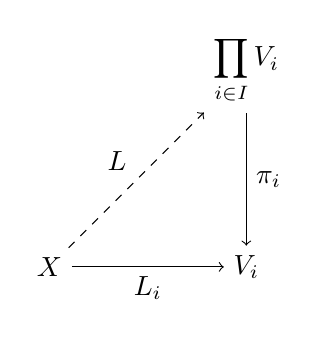
\begin{tikzpicture}[node distance=2.5cm, auto]
	\node (P) {$\displaystyle\prod_{i \in I} \bm{V_i}$};
	\node (Ci) [below of=P] {$\bm{V_i}$};
	\node (X) [left of=Ci] {$\bm X$};
	\draw[->] (X) to node [swap] {$L_i$} (Ci);
	\draw[->, dashed] (X) to node {$L$} (P);
	\draw[->] (P) to node {$\pi_i$} (Ci);
\end{tikzpicture}
\end{figure}
\end{prop}
\begin{proof}
Defina a função \func{L}{X}{\prod_{i \in I} V_i}{x}{(L_i(x))_{i \in I}.} Da propriedade universal para conjuntos, $L$ é a única função de $X$ para $\bigtimes_{i \in I} \bm{V_i}$ tal que, para todo $i \in I$, $\pi_i \circ L = L_i$. Falta mostrar que $L$ é transformação linear. Sejam $c \in C$ e $x_1,x_2 \in V$. Então
	\begin{align*}
	L(x_1+cx_2) &= (L_i(x_1+cx_2))_{i \in I} \\
		&= (L_i(x_1)+cL_i(x_2))_{i \in I} \\
		&= (L_i(x_1))_{i \in I}+c(L_i(x_2))_{i \in I} \\
		&= L(x_1)+cL(x_2). \qedhere
	\end{align*}
\end{proof}

\subsection{Coproduto (Soma)}

\begin{defi}
Seja $(\bm{V_i})_{i \in I} = ((V_i,+_i,\cdot_i))_{i \in I}$ uma família de espaços vetoriais. A \emph{soma categórica} de $(\bm{V_i})_{i \in I}$ é
	\begin{equation*}
	\coprod_{i \in I} \bm{V_i} = (V,+,\cdot),
	\end{equation*}
em que $V = \set{(v_i)_{i \in I} \in \prod_{i \in I} V_i}{\exists J \subseteq I \qquad \card{J} < \card{\N} \e v_i \neq 0}$,
	\begin{align*}
	+: V \times V &\to V \\
			(v_1,v_2) &\mapsto ((v_1)_i +_i (v_2)_i)_{i \in I}
	\end{align*}
e
	\begin{align*}
	\cdot: C \times V &\to V \\
			(c,v) &\mapsto (c(v)_i)_{i \in I}.
	\end{align*}
\end{defi}

Observe que, se $\card{I} < \card{\N}$, então $\prod_{i \in I} \bm{V_i} = \coprod_{i \in I} \bm{V_i}$.

\begin{prop}[Propriedade Universal]
Sejam $(\bm{V_i})_{i \in I}$ uma família de espaços vetoriais sobre um corpo $\bm C$, $\bm X$ um espaço vetorial sobre $\bm C$ e, para todo $i \in I$, $L_i: \bm{V_i} \to \bm X$ uma transformação linear. Então existe única transformação linear $L: \bm X \to \coprod_{i \in I} \bm{V_i}$ tal que, para todo $i \in I$, $L \circ \iota_i = L_i$ (o diagrama comuta).
\begin{figure}
\centering
\begin{tikzpicture}[node distance=2.5cm, auto]
	\node (Ci) {$\bm{V_i}$};
	\node (S) [below of=Ci] {$\displaystyle\coprod_{i \in I} \bm{V_i}$};
	\node (X) [right of=Ci] {$\bm X$};
	\draw[->] (Ci) to node {$L_i$} (X);
	\draw[->, dashed] (S) to node [swap] {$L$} (X);
	\draw[->] (Ci) to node [swap] {$\iota_i$} (S);
\end{tikzpicture}
\end{figure}
\end{prop}

O coproduto de espaços vetoriais é também chamado de \emph{soma} ou \emph{soma direta} e denotado
	\begin{equation*}
	\bigoplus_{i \in I} \bm{V_i}.
	\end{equation*}


























\chapter{Álgebra Multilinear}

\section{Transformações Multilineares}

\begin{defi}
Sejam $\bm{V_0},\cdots,\bm{V_{n-1}}$ e $\bm W$ espaços lineares sobre um corpo $\bm C$. Uma \emph{transformação $n$-linear} de $(\bm{V_0},\ldots,\bm{V_{n-1}})$ para $\bm W$ é uma função
	\begin{equation*}
	T: \bm V_0 \times \cdots \times \bm V_{n-1} \to \bm W
	\end{equation*}
tal que, para todo $i \in n$ e $(\bm v_0,\ldots,\bm v_{i-1},\bm v_{i+1},\ldots,\bm v_{n-1}) \in \bm{V_0} \times \cdots \times \bm{V_{i-1}} \times \bm{V_{i+1}} \times \cdots \times \bm V_{n-1}$, a função
\func{T(\bm v_0,\ldots,\bm v_{i-1},\var,\bm v_{i+1},\ldots,\bm v_{n-1})}{\bm{V_i}}{\bm W}{\bm v}{T(\bm v_0,\ldots,\bm v_{i-1},\bm v,\bm v_{i+1},\ldots,\bm v_{n-1})}
%\func{T(\bm v_0,\ldots,\underbrace{\var}_i,\ldots,\bm v_{n-1})}{\bm{V_i}}{\bm W}{\bm v}{T(\bm v_0,\ldots,\underbrace{\bm v}_i,\ldots,\bm v_{n-1})}
é uma transformação linear. O conjunto dessas transformações é denotado
	\begin{equation*}
	\lin(\bm{V_0},\ldots,\bm{V_{n-1}};\bm W)
	\end{equation*}
e, quando todos os espaços $\bm{V_i}$ são iguais, denota-se
	\begin{equation*}
	\lin^n(\bm V;\bm W) \coloneqq \lin(\underbrace{\bm V,\ldots,\bm V}_n;\bm W)
	\end{equation*}
\end{defi}

\begin{prop}
Sejam $\bm{V_0},\cdots,\bm{V_{n-1}}$ e $\bm W$ espaços lineares de dimensão finita sobre um corpo $\bm C$ cujas dimensões são $d_0,\ldots,d_{n-1}$ e $d$, respectivamente, e, para cada $i \in n$, seja $(\bm b_{ij})_{j \in d_i}$ uma base ordenada de $\bm{V_i}$. Então toda transformação $n$-linear $T \in \lin(\bm{V_0},\ldots,\bm{V_{n-1}};\bm W)$ está determinada pelos seus valores em $(\bm b_{0j_0},\ldots,\bm b_{(n-1)j_{n-1}})$.
\end{prop}
\begin{proof}
Como consequência da propriedade de linearidade generalizada para transformações lineares, para todos $\bm v_0,\ldots,\bm v_{m-1} \in \bm{V_k}$ e $c_0,\ldots,c_{m-1} \in C$, vale que
	\begin{equation*}
	T\left(\bm v_0,\ldots,\bigplus_{i \in m} c_i\bm v_i,\ldots,\bm v_{n-1} \right) = \bigplus_{i \in m} c_iT\left(\bm v_0,\ldots,\bm v_i,\ldots,\bm v_{n-1} \right).
	\end{equation*}
Sendo assim, para cada $i \in n$, sejam $\bm v_i \in \bm{V_i}$ e $v_{i0},\ldots,v_{id_i} \in C$ os coeficientes de $\bm v_i$ na base $\bm b_i$, de modo que
	\begin{equation*}
	\bm v_i = \bigplus_{j \in d_i} v_{ij} \bm b_{ij}.
	\end{equation*}
Pela linearidade em cada entrada, temos que
	\begin{align*}
	T(\bm v_0,\ldots,\bm v_{n-1}) &= T\left(\bigplus_{j_0 \in d_0} v_{0j} \bm b_{0j_0},\ldots,\bigplus_{j_{n-1} \in d_{n-1}} v_{(n-1)j_{n-1}} \bm b_{(n-1)j_{n-1}} \right) \\
		&= \bigplus_{j_0 \in d_0} \cdots \bigplus_{j_{n-1} \in d_{n-1}} v_{0j_0} \cdots v_{(n-1)j_{n-1}} T\left(\bm b_{0j_0},\ldots,\bm b_{(n-1)j_{n-1}} \right) \\
		&= \bigplus_{(j_0,\ldots,j_{n-1}) \in d_0 \times \cdots \times d_{n-1}} v_{0j_0} \cdots v_{(n-1)j_{n-1}} T\left(\bm b_{0j_0},\ldots,\bm b_{(n-1)j_{n-1}} \right). 
	\end{align*}
Portanto a função $T$ está determinada pelos valores que tem nos elementos
	\begin{equation*}
	(\bm b_{0j_0},\ldots,\bm b_{(n-1)j_{n-1}}).
	\end{equation*}
Como há $d_0 \cdots d_{n-1}$ desses elementos, há essa quantidade de escolhas a serem determinadas para se determinar os valores de $T$.
\end{proof}

\begin{prop}
Sejam $\bm{V_1},\cdots,\bm{V_n}$ e $\bm W$ espaços lineares sobre um corpo $\bm C$. Então
	\begin{equation*}
	\bm{\lin(\bm{V_1},\ldots,\bm{V_n};\bm W)} \coloneqq (\lin(\bm{V_1},\ldots,\bm{V_n};\bm W),+,\cdot),
	\end{equation*}	
em que $+$ e $\cdot$ são a soma e o produto escalar pontuais induzidos por $\bm W$, é um espaço linear sobre $\bm C$ (de dimensão ...).
\end{prop}

\section{Formas Multilineares}

\begin{defi}
Seja $\bm V$ um espaço linear sobre um corpo $\bm C$. Uma \emph{forma $k$-linear} em $\bm V$ é uma função $f \in \lin^k(\bm V;\bm C)$, ou seja, um funcional $k$-linear em $(\bm V,\ldots,\bm V)$.
\end{defi}

\begin{defi}
Seja $\bm V$ um espaço linear sobre um corpo $\bm C$. Uma forma $k$-linear $f$ em $\bm V$ é:
\begin{enumerate}
\item \emph{simétrica} se, e somente se, para toda permutação $p \in \sime_k$ e todos $\bm v_0,\ldots,\bm v_{k-1} \in V$,
	\begin{equation*}
	f(\bm v_{p(0)},\ldots,\bm v_{p(k-1)}) = f(\bm v_0,\ldots,\bm v_{k-1});
	\end{equation*}
\item \emph{antissimétrica} se, e somente se, para toda permutação $p \in \sime_k$ e todos $\bm v_0,\ldots,\bm v_{k-1} \in V$,
	\begin{equation*}
	f(\bm v_{p(0)},\ldots,\bm v_{p(k-1)}) = \prd(p) f(\bm v_0,\ldots,\bm v_{k-1});
	\end{equation*}
\item \emph{alternada} se, e somente se, para todos $\bm v_0,\ldots,\bm v_{k-1} \in V$ linearmente dependentes,
	\begin{equation*}
	f(\bm v_0,\ldots,\bm v_{k-1}) = 0.
	\end{equation*}
\end{enumerate}
O conjunto das formas $k$-lineares alternadas é denotado $\mathcal A^k(\bm V)$.
\end{defi}

\begin{prop}
Sejam $\bm V$ um espaço linear sobre um corpo $\bm C$ e $f \in \lin^k(\bm V;\bm C)$.
\end{prop}

\begin{prop}
Seja $\bm V$ um espaço linear sobre um corpo $\bm C$. Então
\begin{enumerate}
\item Uma forma $k$-linear em $\bm V$ é alternada se, e somente se, para todos $\bm v_0,\ldots,\bm v_{k-1} \in V$ tais que $\bm v_i = \bm v_j$ para dois $i,j \in k$ distintos,
	\begin{equation*}
	f(\bm v_0,\ldots,\bm v_{k-1})=0.
	\end{equation*} 
\item Uma forma alternada $k$-linear em $\bm V$ é antissimétrica. Se a característica de $\bm C$ é diferente de $2$, então uma forma antissimétrica $k$-linear em $\bm V$  é alternada.
\item Se a característica de $\bm C$ é igual a $2$, então uma forma $k$-linear em $\bm V$ é antissimétrica se, e somente se, é simétrica.
\end{enumerate}
\end{prop}
\begin{proof}
\begin{enumerate}
\item Se $f$ é alternada, então, para todos $\bm v_0,\ldots,\bm v_{k-1} \in V$ tais que $\bm v_i = \bm v_j$ para dois $i,j \in k$ distintos, o conjunto $\{\bm v_0,\ldots,\bm v_{k-1}\}$ é linearmente dependente, portanto $f(\bm v_0,\ldots,\bm v_{k-1})=0$. Reciprocamente, suponha que $f$ satisfaz a propriedade e sejam $\bm v_0,\ldots,\bm v_{k-1} \in V$ linearmente dependentes. Então existe $i \in k$ tal que $\bm v_i$ é combinação linear dos outros $\bm v_j$: existem $c_j \in C$, $j \in k\setminus\{i\}$, tais que
	\begin{equation*}
	\bm v_i = \bigplus_{j \in k\setminus\{i\}} c_j \bm v_j.
	\end{equation*}
Assim, segue da $k$-linearidade e da propriedade que
	\begin{align*}
	f(\bm v_0,\ldots,\bm v_{k-1}) &= f\left(\bm v_0,\ldots, \bigplus_{j \in k\setminus\{i\}} c_j \bm v_j,\ldots,\bm v_{k-1}\right) \\
		&= \bigplus_{j \in k\setminus\{i\}} c_j f(\bm v_0,\ldots, \bm v_j,\ldots,\bm v_{k-1}) \\
		&=\bigplus_{j \in k\setminus\{i\}} c_j 0 = 0.
	\end{align*}

\item Suponha $f$ alternada e sejam $\bm v_0,\ldots,\bm v_{k-1} \in V$. Então segue da $k$-linearidade e da alternância de $f$ que
	\begin{align*}
	0 =&f(\bm v_0,\ldots,\bm v_i+\bm v_j,\ldots,\bm v_i+\bm v_j,\ldots,\bm v_{k-1}) \\
		=& f(\bm v_0,\ldots,\bm v_i,\ldots,\bm v_i,\ldots,\bm v_{k-1}) + f(\bm v_0,\ldots,\bm v_i,\ldots,\bm v_j,\ldots,\bm v_{k-1}) \\
		&+f(\bm v_0,\ldots,\bm v_j,\ldots,\bm v_i,\ldots,\bm v_{k-1}) + f(\bm v_0,\ldots,\bm v_j,\ldots,\bm v_j,\ldots,\bm v_{k-1}) \\
		=& f(\bm v_0,\ldots,\bm v_i,\ldots,\bm v_j,\ldots,\bm v_{k-1}) +f(\bm v_0,\ldots,\bm v_j,\ldots,\bm v_i,\ldots,\bm v_{k-1}),
	\end{align*}
portanto
	\begin{equation*}
	f(\bm v_0,\ldots,\bm v_i,\ldots,\bm v_j,\ldots,\bm v_{k-1}) = - f(\bm v_0,\ldots,\bm v_j,\ldots,\bm v_i,\ldots,\bm v_{k-1}).
	\end{equation*}
Como toda permutação $p \in \sime_k$ é um produto de $N \in \N$ inversões, e como $\prd(p)=(-1)^N$, segue por indução que, para toda permutação $p \in \sime_k$,
	\begin{equation*}
	f(\bm v_{p(0)},\ldots,\bm v_{p(k-1)}) =(-1)^N f(\bm v_0,\ldots,\bm v_{k-1}) = \prd(p) f(\bm v_0,\ldots,\bm v_{k-1}).
	\end{equation*}

Suponha que a característica de $\bm C$ é diferente de $2$. Sejam $f$ uma forma antissimétrica $k$-linear em $\bm V$ e sejam $\bm v_0,\ldots,\bm v_{k-1} \in V$ tais que $\bm v_i = \bm v_j$ para dois $i,j \in k$ distintos. Considerando a permutação $(i \quad j) \in \sime_k$, segue da antissimetria de $f$ e de $\prd((i \quad j))=-1$ que
	\begin{align*}
	f(\bm v_0,\ldots,\bm v_i,\ldots,\bm v_j,\ldots,\bm v_{k-1}) &= f(\bm v_0,\ldots,\bm v_j,\ldots,\bm v_i,\ldots,\bm v_{k-1}) \\
		&= - f(\bm v_0,\ldots,\bm v_i,\ldots,\bm v_j,\ldots,\bm v_{k-1}),
	\end{align*}
portanto
	\begin{equation*}
	2 f(\bm v_0,\ldots,\bm v_{k-1})=0.
	\end{equation*}
Como a característica de $\bm C$ é diferente de $2$, segue que $f(\bm v_0,\ldots,\bm v_{k-1})=0$. Do item 1 segue que $f$ é alternada.

\item Se a característica de $\bm C$ é igual de $2$, então $-1=1$. Isso implica que, para qualquer permutação $p$, $\prd(p)=1$.
\end{enumerate}
\end{proof}

\section{Produto Exterior}

\begin{defi}
Sejam $\bm V$ um espaço linear sobre um corpo $\bm C$, $f \in \mathcal{A}^k(\bm V)$, $g \in \mathcal{A}^l(\bm V)$ e $\bm v_0,\ldots,\bm v_{k+l-1} \in \bm V$. O \emph{produto exterior} entre $f$ e $g$ em $(\bm v_0,\ldots,\bm v_{k+l-1})$ é
	\begin{equation*}
	(f \wedge g)(\bm v_0,\ldots,\bm v_{k+l-1}) \coloneqq \frac{1}{k!l!} \bigplus_{p \in \sime_{k+l}} \prd(p) f(\bm v_0,\ldots,\bm v_{k-1})g(\bm v_k,\ldots,\bm v_{k+l-1})
	\end{equation*}
\end{defi}

\begin{prop}
Sejam $\bm V$ um espaço linear de dimensão finita $d$ sobre um corpo $\bm C$, $(\bm b_i)_{i \in d}$ um base ordenada de $\bm V$ e $(\bm b^*_i)_{i \in d}$ sua base dual de $\bm{V^*}$. Então $\mathcal{A}^k(\bm V)$ é um espaço linear sobre $\bm C$ de dimensão $\binom{d}{k}$ e o conjunto
	\begin{equation*}
	\set{\bm b^*_{i_0} \wedge \cdots \wedge \bm b^*_{i_{k-1}}}{i_0 < \cdots < i_{k-1} \in d}
	\end{equation*}
de formas alternadas $k$-lineares em $\bm V$ é uma base para $\mathcal{A}^k(\bm V)$
\end{prop}

Em particular, isso mostra que formas $d$-lineares num espaço de dimensão $d$ são todas múltiplos umas das outras, pois $\binom{d}{d}=1$. Podemos fixar o valor de uma das formas como 1 e chamá-la de \emph{determinante}.

















\chapter{Álgebras Booleanas}

\begin{defi}
Uma \emph{álgebra booleana} é uma tripla $(A, \vee ,\wedge)$, em que $A$ é um conjunto não vazio, que satisfaz
	\begin{enumerate}
	\item $(A, \vee )$ e $(A,\wedge)$ são magmas comutativos com elementos neutros $0$ e $1$, respectivamente;
	\item As operações $ \vee $ e $\wedge$ são distributivas uma sobre a outra;
	\item Todo elemento de $a_1 \in A$ tem um elemento \emph{complementar} $a_2 \in A$ que satisfaz $a_1 \vee a_2=1$ e $a_1 \wedge a_2 = 0$.
	\end{enumerate}
\end{defi}

\begin{prop}
\label{prop:algeb.subconj}
	Seja $A$ um conjunto e $\mathcal A \subseteq \p(A)$ um conjunto de partes de $A$ que satisfaz
	\begin{enumerate}
	\item $\emptyset \in \mathcal A$;
	\item $X \in \mathcal A \Rightarrow X^\complement \in \mathcal A$.
	\end{enumerate}
Então $(\mathcal A,\cup,\cap)$ é uma álgebra booleana.
\end{prop}
\begin{proof}
	Primeiramente, é necessário notar, embora os símbolos $\cup$ e $\cap$ não sejam funções propriamente ditas, ao fixarmos um conjunto $A$, podemos definir $\cup$ e $\cap$ como operações binárias em $\p(A)$, dadas por $(X,Y) \mapsto X \cup Y$ e $(X,Y) \mapsto X \cap Y$, respectivamente. Para $X,Y \in \mathcal A$, temos que $X \cup Y,X \cap Y \in \mathcal A$, o que mostra que as operações estão bem definidas.

	Sendo assim, podemos prosseguir com a demonstração. Se $\mathcal A$ satisfaz as propriedades do enunciado, então $A = \emptyset^\complement \in \mathcal A$. O par $(\mathcal A,\cup)$ é um magma comutativo com elemento neutro $\emptyset$, pois a união de dois cojuntos é comutativa por definição e a união de um conjunto qualquer com o conjunto vazio dá o próprio conjunto. Da mesma forma, o par $(\mathcal A,\wedge)$ é um magma comutativo com elemento neutro $A$, pois a interseção de dois conjuntos é comutativa por definição e a interseção de qualquer conjunto com o conjunto $A$ é o próprio conjunto. Ainda, vale que, para todo $X,Y,Z \in \mathcal A$, $X \cup (Y \cap Z) = (X \cup Y) \cap (X \cup Z)$ e $X \cap (Y \cup Z) = (X \cap Y) \cup (X \cap Z)$; ou seja, as operações binárias $\cup$ e $\cap$ são distributivas uma sobre a outra. Por fim, nota-se que, dado $X \in \mathcal A$, $X^\complement \in \mathcal A$ e vale $X \cup X^\complement = A$ e $X \cap X^\complement = \emptyset$. Logo $(\mathcal A,\cup,\cap)$ é uma álgebra booleana.
\end{proof}

\begin{prop}[Princípio da Dualidade]
	Toda afirmação dudutível somente a partir da definição de álgebra booleana continua válida se são trocados entre si os símbolos $ \vee $ e $\wedge$ e os símbolos $0$ e $1$ que aparecem na expressão.
\end{prop}
\begin{proof}
	Todas as propriedades de uma álgebra booleana são definidas simetricaente e continuam iguais se trocamos entre si os símbolos $ \vee $ e $\wedge$ e os símbolos $0$ e $1$. Logo isso também vale para qualquer afirmação dedutível dessas propriedades.
\end{proof}

	Como consequência do princípio da dualidade, qualquer afirmação dedutível das pripriedades de álbegra booleana tem uma afirmação associadad a ela ao trocarmos entre si os símbolos $ \vee $ e $\wedge$ e os símbolos $0$ e $1$, que chamaremos que sua afirmação \emph{dual}. Claramente, a afirmação dual da dual é a própria afirmação. Portanto só será necessário demonstrar a afirmação para demonstrar sua afirmação dual. Toda proposição, lema e teorema dessa seção exibirá sua proposição, lema e teorema dual, mas a afirmação dual não será demonstrada.

\begin{teo}[Operações com Identidades]
	Seja $(A, \vee ,\wedge)$ uma álgebra booleana. Então
	\begin{equation*}
	\forall a \in A \qquad a \vee 1=1
	\end{equation*}
	\begin{equation*}
	\forall a \in A \qquad a \wedge 0 = 0
	\end{equation*}
\end{teo}

\begin{teo}[Leis de Absorção]
	Seja $(A, \vee ,\wedge)$ uma álgebra booleana. Então
	\begin{equation*}
	\forall a,b \in A \qquad a \vee (a \wedge b)=a
	\end{equation*}
	\begin{equation*}
	\forall a,b \in A \qquad a \wedge (a  \vee  b) = a
	\end{equation*}
\end{teo}

\begin{coro}[Leis da Tautologia]
	Seja $(A, \vee ,\wedge)$ uma álgebra booleana. Então
	\begin{equation*}
	\forall a \in A \qquad a \vee a=a
	\end{equation*}
	\begin{equation*}
	\forall a \in A \qquad a \wedge a = a
	\end{equation*}
\end{coro}
\begin{proof}
	Basta tomar $b=1$ e $b=0$ nas proposições anteriores.
\end{proof}

\begin{teo}[Associatividade]
	Seja $(A, \vee ,\wedge)$ uma álgebra booleana. Então
	\begin{equation*}
	(A, \vee ) \text{ é associativo.}
	\end{equation*}
	\begin{equation*}
	(A,\wedge) \text{ é associativo.}
	\end{equation*}
\end{teo}

\begin{teo}[Unicidade do Complementar]
	Seja $(A, \vee ,\wedge)$ uma álgebra booleana e $a \in A$. Então o complementar de $a$ é único.
\end{teo}

	Note que esse teorema é seu próprio dual.

\begin{teo}[Dupla Complementação]
	Seja $(A, \vee ,\wedge)$ uma álgebra booleana e $a \in A$. Então o complementar de $a'$ é $a$.
\end{teo}

\begin{teo}[Identidades Complementares]
	Seja $(A, \vee ,\wedge)$ uma álgebra booleana. Então
	\begin{equation*}
	0'=1
	\end{equation*}
	\begin{equation*}
	1'=0
	\end{equation*}
\end{teo}

\begin{teo}[Leis de De Morgan]
\label{prop:de.morgan}
	Seja $(A, \vee ,\wedge)$ uma álgebra booleana. Então
	\begin{equation*}
	\forall a,b \in A \qquad (a \wedge b)'=a' \vee b'
	\end{equation*}
	\begin{equation*}
	\forall a,b \in A \qquad (a  \vee  b)'=a' \wedge b'
	\end{equation*}
\end{teo}